\documentclass[11pt,twoside]{book}

\usepackage[utf8]{inputenc}
\usepackage[T1]{fontenc}
\usepackage[spanish,es-noshorthands,es-tabla]{babel}
\usepackage{graphicx}
\usepackage{xurl}
\usepackage[strings]{underscore}
\usepackage{expl3}
\usepackage{eso-pic}
\usepackage{ragged2e}
\usepackage{float}
\usepackage{array}
\usepackage{longtable}
\usepackage[print,doble]{UAL}
\usepackage{codigo}
\usepackage{rotating}

% Permite saltos de línea dentro de identificadores en \texttt{...} (camelCase/PascalCase y letra<->número)
\ExplSyntaxOn
\cs_new_protected:Npn \asc_allowbreak_texttt:n #1
	{
		\tl_set:Nn \l_tmpa_tl {#1}
		% Separa acrónimos seguidos de palabra: AIEnabled -> AI\allowbreak Enabled
		\regex_replace_all:nnN {([A-Z])([A-Z][a-z])} {\1\c{allowbreak}\2} \l_tmpa_tl
		% Separa límites camelCase/PascalCase: tilemapCollider -> tilemap\allowbreak Collider
		\regex_replace_all:nnN {([a-z])([A-Z])} {\1\c{allowbreak}\2} \l_tmpa_tl
		% Separa límites letra<->número: Collider2D -> Collider\allowbreak 2\allowbreak D
		\regex_replace_all:nnN {([A-Za-z])([0-9])} {\1\c{allowbreak}\2} \l_tmpa_tl
		\regex_replace_all:nnN {([0-9])([A-Za-z])} {\1\c{allowbreak}\2} \l_tmpa_tl
		\tl_use:N \l_tmpa_tl
	}
\cs_new_eq:NN \asc_orig_texttt \texttt
\protected\def\texttt#1{\asc_orig_texttt{\asc_allowbreak_texttt:n{#1}}}
\ExplSyntaxOff

% Título de tabla fuera del entorno float: mantiene numeración y añade entrada al índice.
\newcommand{\TablaTitulo}[1]{%
	\refstepcounter{table}%
	\addcontentsline{lot}{table}{\protect\numberline{\thetable}#1}%
	\textbf{Tabla \thetable.} #1%
}

% Bibliografía
\usepackage[numbers,square]{natbib}
\bibliographystyle{IEEEtran}

\author{Naoufal Saidi Hassani}
\titulo{Desarrollo de un videojuego roguelike 2D con generación procedural en Unity}
\subTitulo{DEPARTAMENTO DE INFORMÁTICA\\ ÁREA DE LENGUAJES Y SISTEMAS INFORMÁTICOS}
\estudios{Grado en Informática}
\universidad{UNIVERSIDAD DE ALMERÍA}
\director{Nicolás Padilla Soriano}
\direct{Javier Criado Rodríguez}
\curso{2025/2026}

\pagestyle{cab}
\raggedbottom

\begin{document}

% ========= FRONTMATTER =========
\frontmatter

\portada

\begin{dedicatoria}
Dedicado a mi familia, por su apoyo incondicional y su amor constante, que han sido mi fuerza motriz en cada paso de este viaje académico.
\end{dedicatoria}

%%%%%%%%%%%%%%%%%%%%%%%%%%%%%%%%%%%%%%%%%%%%%%%%%%%%%%%%%%%%%%%%%%%%%%%%%%%%
%%%%%%%%%%%%%%% TABLA DE CONTENIDOS, ÍNDICES Y ABREVIATURAS %%%%%%%%%%%%%%%%%
%%%%%%%%%%%%%%%%%%%%%%%%%%%%%%%%%%%%%%%%%%%%%%%%%%%%%%%%%%%%%%%%%%%%%%%%%%%%

%---------------------------------------------------------------------------
% Configuración de profundidad
%---------------------------------------------------------------------------

\setcounter{secnumdepth}{2}
\setcounter{tocdepth}{2}

%---------------------------------------------------------------------------
% Tabla de contenidos
%---------------------------------------------------------------------------

\addtocontents{toc}{~\hfill\small{Página}\par}
\addtocontents{toc}{\vspace{2pt} \hrule \vspace{5mm} \par}

\tableofcontents
\clearpage

%---------------------------------------------------------------------------
% Índices
%---------------------------------------------------------------------------

\listoffigures
\clearpage

%---------------------------------------------------------------------------
% Relación de abreviaturas y acrónimos
%---------------------------------------------------------------------------

\section*{ABREVIATURAS}
\addcontentsline{toc}{section}{ABREVIATURAS}

\vspace{0.3cm}

\begin{tabular}{ l | l }
    & \\
    AI   & Artificial Intelligence \\
    ESI  & Escuela Superior de Ingeniería \\
    GPC  & Generación Procedural de Contenido \\
    IA   & Inteligencia Artificial \\
    InSo & Ingeniería del Software \\
    PNJ  & Personaje No Jugador \\
    SBSE & Search Based Software Engineering \\
    TFG  & Trabajo Fin de Grado \\
    UAL  & Universidad de Almería \\
    & \\
\end{tabular}

\clearpage


\addcontentsline{toc}{chapter}{Resumen y Abstract}
\chapter*{Resumen y Abstract}
Este Trabajo de Fin de Grado presenta Ascension, un videojuego 2D roguelike desarrollado en Unity. El sistema implementa generación procedural, IA enemiga, gestión de estados y un sistema de puntuación. La arquitectura utiliza ScriptableObjects y patrones de diseño (Singleton, Observer, Strategy, Template Method) para asegurar el desacoplamiento y la mantenibilidad del código. Los resultados confirman una solución robusta y extensible, con mejoras futuras previstas en el diseño de jefes finales y el sistema de audio.

\vspace{1.5cm}

\textbf{Abstract.} This thesis presents Ascension, a 2D roguelike game developed in Unity. The system features procedural generation, enemy AI, state management, and score tracking. The architecture employs ScriptableObjects and design patterns (Singleton, Observer, Strategy, Template Method) to ensure modularity and maintainability. Results demonstrate a robust and extensible architecture, with future work focusing on boss integration and the audio systems.

% ========= CUERPO =========
\mainmatter
\marcagua

\chapter{Introducción}


\section{Contexto}


La industria del videojuego se ha consolidado durante las últimas décadas como uno de los sectores tecnológicos de mayor crecimiento a nivel mundial. En 2020, el mercado global de videojuegos generó ingresos estimados de 159.300 millones de dólares \cite{NEWZOO_GLOBAL_GAMES_MARKET_REPORT_2020_LIGHT}. Esta magnitud económica, unida a la constante evolución tecnológica del sector, convierte el desarrollo de videojuegos en un campo de estudio relevante para la ingeniería informática.

Desde la perspectiva de la ingeniería del software, el desarrollo de videojuegos plantea desafíos técnicos de considerable complejidad. Entre ellos destacan la arquitectura de sistemas en tiempo real, la implementación de algoritmos de inteligencia artificial, la generación procedural de contenido (creación automática de elementos del juego mediante algoritmos) y el diseño de interfaces interactivas. Este contexto convierte el desarrollo de un videojuego en un ámbito adecuado para la realización de un Trabajo de Fin de Grado (TFG) en Ingeniería Informática, al permitir la aplicación práctica e integrada de conocimientos adquiridos durante la formación académica en áreas como la programación orientada a objetos, las estructuras de datos, la arquitectura de software y la ingeniería del software.

Los videojuegos pertenecientes al subgénero \textit{roguelike} presentan una serie de características técnicas que los convierten en un objeto de estudio de especial interés desde el punto de vista de la ingeniería. Entre dichas características destacan la generación procedural de niveles, la ausencia de persistencia del progreso entre partidas -- lo que se conoce como \textit{permadeath} o muerte permanente --, la progresión limitada a cada ejecución del juego y una elevada rejugabilidad derivada de la variabilidad del contenido generado. Estas propiedades obligan a diseñar sistemas software capaces de producir escenarios jugables, coherentes y equilibrados de forma automática, sin intervención manual directa por parte de un diseñador de niveles.

En este contexto se plantea el siguiente problema técnico: cómo diseñar e implementar una arquitectura de software modular que permita la generación automática de niveles jugables, la gestión concurrente de múltiples subsistemas -- como la inteligencia artificial de los enemigos, el motor de físicas, la interfaz de usuario (UI) o el control de estados del juego -- y la parametrización del contenido de manera escalable y mantenible. Este problema resulta representativo de los retos que afronta la ingeniería del software aplicada al desarrollo de sistemas interactivos en tiempo real.

\section{Motivación y justificación}


La elección de un videojuego del subgénero \textit{roguelike} como objeto del presente Trabajo de Fin de Grado responde a una doble motivación: académica y técnica.

Desde el punto de vista académico, el desarrollo de un videojuego constituye un dominio de aplicación que permite integrar de forma práctica las competencias adquiridas a lo largo del Grado en Ingeniería Informática. En particular, el proyecto ofrece un marco adecuado para aplicar los contenidos estudiados en asignaturas clave de la titulación:

\begin{itemize}
\item \textbf{Ingeniería del Software (INSO).} Los patrones de diseño de software -- \textit{Singleton}, \textit{Observer}, \textit{Strategy} y \textit{Template Method} --, la captura de requisitos mediante historias de usuario, la arquitectura modular basada en la separación entre datos configurables y lógica de ejecución, y la gestión del ciclo de vida del software mediante una metodología iterativa e incremental constituyen contenidos propios de esta asignatura que se aplican de forma directa en el proyecto.
\item \textbf{Programación Orientada a Objetos.} La jerarquía de clases del sistema de enemigos (\texttt{Enemy} -> \texttt{SlimeGreen} / \texttt{SlimeRed} / \texttt{SlimeBlue}) y del sistema de armas (\texttt{Weapon} -> \texttt{MeleeWeapon} / \texttt{RangedWeapon}) aplica los principios de herencia, polimorfismo y encapsulamiento. El patrón \textit{Template Method}, que define comportamiento base en la clase padre y delega la especialización en las subclases, constituye un ejemplo representativo de la aplicación de estos conceptos.
\item \textbf{Algoritmia y Estructuras de Datos.} La generación procedural de salas, el algoritmo de expansión por \textit{clusters} (agrupaciones contiguas de tiles) para la distribución de tiles especiales, la generación ponderada de enemigos mediante presupuesto de coste y el control del flujo del juego mediante máquinas de estados constituyen problemas algorítmicos no triviales que permiten demostrar competencias en esta área.
\item \textbf{Diseño de Sistemas Interactivos.} La implementación de la interfaz de usuario -- sistema de corazones, menú de pausa, pantallas de fin de partida -- y la atención a la experiencia de juego mediante retroalimentación visual (parpadeo de invulnerabilidad, parpadeo rojo de muerte, efectos de impacto) se vinculan con los contenidos de diseño de interacción y usabilidad.
\end{itemize}

Esta vinculación con la Ingeniería del Software resulta especialmente significativa. El desarrollo de un videojuego \textit{roguelike} no se limita a la escritura de código: requiere definir una arquitectura de software modular, aplicar patrones de diseño reconocidos, gestionar la separación entre datos configurables y lógica de ejecución mediante mecanismos como los \textit{ScriptableObjects} (activos de datos serializables de Unity que permiten configurar parámetros desde el inspector del motor sin modificar el código fuente), y seguir una metodología de desarrollo que permita validar el producto de forma progresiva. Estos principios coinciden con los que articulan la disciplina de la Ingeniería del Software, lo que convierte el proyecto en un ejercicio representativo de las competencias que esta asignatura desarrolla.

Desde el punto de vista técnico, el subgénero \textit{roguelike} presenta una complejidad que lo convierte en un objeto de estudio adecuado para un Trabajo de Fin de Grado. La generación procedural de contenido obliga a diseñar algoritmos capaces de producir entornos jugables, coherentes y equilibrados sin intervención manual. La coordinación de múltiples subsistemas en tiempo real -- combate, inteligencia artificial, generación de niveles, interfaz de usuario -- exige una arquitectura con separación de responsabilidades y bajo acoplamiento entre componentes. Asimismo, la naturaleza iterativa del desarrollo de videojuegos, donde las mecánicas se ajustan mediante ciclos de prueba y refinamiento, se alinea con las metodologías de desarrollo incremental estudiadas durante la formación académica.

La relevancia cultural e industrial del subgénero refuerza la pertinencia de esta elección. Títulos como \textit{Hades} (Supergiant Games, 2020), \textit{Dead Cells} (Motion Twin, 2018), \textit{The Binding of Isaac} (Edmund McMillen, 2011) o \textit{Enter the Gungeon} (Dodge Roll, 2016) se han consolidado como referencias contemporáneas del subgénero. Por ejemplo, \textit{Hades} ha recibido reconocimiento en premios de la industria; en \textit{The Game Awards} 2020 obtuvo el galardón a Mejor Juego Independiente \cite{CNET_GAME_AWARDS_2020_WINNERS}. El análisis de estos sistemas permite abordar conceptos avanzados de ingeniería del software en un contexto práctico y representativo.

\section{Objetivos}


\subsection{Objetivo general}


El objetivo general del proyecto es diseñar, implementar y documentar un videojuego \textit{roguelike} funcional que permita evidenciar la aplicación de principios de ingeniería del software en el ámbito del desarrollo de videojuegos, con especial énfasis en la arquitectura modular y la generación procedural de contenido.

\subsection{Objetivos específicos}


De este objetivo general se derivan los siguientes objetivos específicos (OE):

\begin{enumerate}
\item \textbf{OE-1.} Diseñar e implementar una arquitectura modular basada en patrones de diseño (\textit{Singleton}, \textit{Observer}, \textit{Strategy}, \textit{Template Method}) que facilite la separación de responsabilidades entre subsistemas y promueva la mantenibilidad y extensibilidad del código.
\item \textbf{OE-2.} Desarrollar un algoritmo de generación procedural de salas que garantice la jugabilidad y la coherencia espacial del entorno, incluyendo la distribución de tiles especiales mediante clusters, la colocación de muros con colisionadores y el posicionamiento de escaleras de transición.
\item \textbf{OE-3.} Implementar tres comportamientos diferenciados de inteligencia artificial para los enemigos (persecución, ataque a distancia y aproximación por saltos) y un sistema de enemigos especiales con atributos escalados que actúen como jefes periódicos.
\item \textbf{OE-4.} Crear un sistema de armas con mecánicas de combate cuerpo a cuerpo y a distancia, incluyendo detección de colisiones, proyectiles físicos y un sistema de órbita del arma alrededor del jugador orientado hacia la posición del cursor.
\item \textbf{OE-5.} Implementar un sistema de tiles con efectos que modifiquen la jugabilidad, incluyendo su configuración mediante \textit{ScriptableObjects} y su distribución controlada en salas generadas proceduralmente.
\item \textbf{OE-6.} Implementar un sistema de persistencia de puntuaciones mediante \textit{PlayerPrefs} con visualización de un ranking en el menú principal, registrando estadísticas completas de cada partida.
\item \textbf{OE-7.} Documentar el proceso de desarrollo, las decisiones técnicas adoptadas y las limitaciones encontradas, exponiendo el trabajo realizado de forma rigurosa y reproducible.
\end{enumerate}

\section{Descripción del proyecto}


El videojuego desarrollado, denominado \textit{Ascension}, es un \textit{roguelike} bidimensional con vista cenital (\textit{top-down}, perspectiva en la que la cámara se sitúa sobre el escenario mirando hacia abajo), en el que el jugador avanza a través de una secuencia de salas generadas de forma procedural, enfrentándose a enemigos hasta alcanzar la condición de victoria establecida. Dicha condición consiste en la derrota de tres enemigos especiales con atributos incrementados -- denominados jefes -- que aparecen de forma periódica cada cinco salas completadas.

El sistema implementado incluye un flujo de juego completo que abarca las siguientes funcionalidades:

\begin{itemize}
\item \textbf{Menú principal} con acceso a la partida, tabla de puntuaciones y opción de salida.
\item \textbf{Selección de clase} entre tres personajes con estadísticas diferenciadas (vida máxima, velocidad de movimiento y arma inicial), lo que permite al jugador adaptar la experiencia a distintos estilos de juego.
\item \textbf{Gestión de estados globales} mediante un \textit{GameManager} (componente gestor central del juego) que coordina las transiciones entre menú, selección de clase, juego activo, pausa, victoria y derrota.
\item \textbf{Generación procedural de salas} mediante un \textit{RoomGenerator} que produce la estructura espacial de cada nivel basándose en \textit{tilemaps} con muros perimetrales, tiles de suelo con variantes visuales, tiles especiales con efectos (hielo, lodo, curación y potenciación de daño) y escaleras de transición entre salas.
\item \textbf{Sistema de combate} que contempla dos tipos de armas: cuerpo a cuerpo, cuyo ataque realiza un barrido angular con detección de colisión, y a distancia, que genera proyectiles físicos dirigidos hacia la posición del cursor. Ambos tipos de arma se configuran mediante \textit{ScriptableObjects} para su parametrización independiente del código.
\item \textbf{Inteligencia artificial de enemigos} con tres comportamientos diferenciados: persecución directa, ataque a distancia con mantenimiento de distancia óptima y aproximación por saltos (\textit{dash}, desplazamientos cortos y rápidos del enemigo hacia el jugador). Cada tipo de enemigo se configura mediante datos almacenados en \textit{ScriptableObjects}, lo que permite parametrizar atributos como velocidad, daño, vida y radio de detección.
\item \textbf{Sistema de gestión de enemigos} que utiliza un algoritmo de generación ponderada por coste, posicionamiento seguro respecto al jugador, limpieza automática de salas y control de interacción con las escaleras en función del estado del combate.
\item \textbf{Interfaz de usuario completa} con visualización dinámica de la salud del jugador mediante corazones, menú de pausa funcional y pantallas de victoria y derrota.
\item \textbf{Sistema de persistencia de puntuaciones} mediante \textit{PlayerPrefs} (almacenamiento local clave–valor proporcionado por Unity) y serialización JSON (\textit{JavaScript Object Notation}, conversión de estructuras de datos a texto estructurado), con un historial de hasta treinta partidas que registra puntuación, clase utilizada, salas completadas, enemigos eliminados, resultado y fecha.
\end{itemize}

El proyecto no incluye un sistema integral de audio ni un controlador genérico de objetos recolectables, al considerarse estos aspectos de menor prioridad para los objetivos académicos del trabajo. Asimismo, el sistema de jefes con fases múltiples y el sistema de generación de armas con rarezas constituyen funcionalidades preparadas a nivel de arquitectura para su extensión futura, pero no se encuentran completamente integradas en el flujo de juego durante la versión actual.

\section{Metodología}


\subsection{Tipo de investigación}


El trabajo se enmarca dentro de una investigación de tipo aplicado, centrada en el diseño e implementación de un producto software funcional. El objetivo principal es demostrar la aplicación práctica de conceptos propios de la ingeniería del software en el contexto del desarrollo de videojuegos, concretamente en la creación de un videojuego bidimensional del subgénero \textit{roguelike}.

\subsection{Metodología de desarrollo de software}


Se ha adoptado una metodología de desarrollo \textbf{iterativa e incremental}, basada en la implementación progresiva de funcionalidades completas y su validación iterativa. Esta decisión se justifica por dos razones fundamentales:

\begin{enumerate}
\item \textbf{Naturaleza exploratoria del proyecto.} El desarrollo de un videojuego requiere experimentar con mecánicas de juego, ajustar parámetros de balance y validar la jugabilidad de forma temprana. Una metodología secuencial (cascada) no permitiría esta flexibilidad.
\item \textbf{Necesidad de adaptación continua.} Durante el desarrollo se identificaron limitaciones técnicas y oportunidades de mejora que exigieron redefinir determinados aspectos del diseño. El enfoque iterativo permitió incorporar estos cambios sin comprometer la estabilidad del sistema.
\end{enumerate}

El proceso de trabajo se estructuró en \textbf{iteraciones de corta duración}, cada una de las cuales generó un incremento funcional del sistema. En cada iteración se llevaron a cabo las siguientes actividades:

\begin{enumerate}
\item \textbf{Diseño} de un subsistema concreto, definiendo su responsabilidad, sus interfaces y sus dependencias con otros módulos.
\item \textbf{Implementación} de la funcionalidad asociada, siguiendo los principios de separación de responsabilidades y bajo acoplamiento.
\item \textbf{Validación} mediante pruebas funcionales manuales en el editor de Unity, comprobando el funcionamiento del subsistema de forma aislada y su integración con los subsistemas existentes.
\item \textbf{Corrección} de errores detectados durante la validación.
\item \textbf{Ajuste del alcance} de iteraciones posteriores en función de los resultados obtenidos y de las prioridades identificadas.
\end{enumerate}

No se ha aplicado una metodología ágil formal como \textit{Scrum} o \textit{Kanban}, dado que el proyecto se ha desarrollado de manera individual. Sin embargo, el enfoque iterativo adoptado comparte principios fundamentales con las metodologías ágiles: entrega frecuente de incrementos funcionales, adaptación al cambio y validación iterativa del producto.

La elección del diseño iterativo se justifica por su adecuación al desarrollo de videojuegos, un ámbito en el que la experimentación, el ajuste de mecánicas y la validación temprana de funcionalidades son factores relevantes para favorecer la viabilidad del producto final y reducir el riesgo técnico. En la práctica, este enfoque permitió, por ejemplo, detectar la necesidad de implementar un sistema de gracia temporal (\textit{grace period}, un breve intervalo tras la aparición en el que el enemigo no puede dañar al jugador), evitando daño instantáneo antes de que el jugador pudiera reaccionar. Este tipo de ajustes, derivados de la validación funcional durante el desarrollo, habría sido difícil de anticipar en una fase de diseño inicial.

\subsection{Proceso de implementación y validación}


La implementación del sistema se llevó a cabo siguiendo un proceso de definición de subsistemas, codificación, pruebas funcionales y refinamiento. Cada componente del videojuego se desarrolló de forma modular e independiente y posteriormente se integró en el sistema global, comprobando su funcionamiento conjunto con los subsistemas ya existentes.

Las iteraciones de desarrollo se organizaron en torno a los siguientes subsistemas, implementados de forma secuencial con solapamientos parciales entre fases:

\begin{enumerate}
\item Gestión central del juego (\textit{GameManager}, máquina de estados, transiciones de escena).
\item Sistema de jugador (movimiento, esquiva, sistema de vida).
\item Generación procedural de salas (\textit{RoomGenerator}, \textit{tilemaps}, colisionadores).
\item Sistema de combate y armas (cuerpo a cuerpo, a distancia, proyectiles).
\item Inteligencia artificial de enemigos (tres comportamientos diferenciados).
\item Sistema de gestión de salas (flujo de progresión, enemigos especiales).
\item Sistema de tiles con efectos (hielo, lodo, curación, potenciación).
\item Interfaz de usuario (corazones, puntuación, menú de pausa, pantallas finales).
\item Sistema de persistencia (puntuaciones, historial de partidas).
\end{enumerate}

El proceso de validación se basó en pruebas funcionales manuales ejecutadas directamente en el editor de Unity. En cada iteración se comprobaron aspectos clave del sistema, entre los que se incluyen:

\begin{itemize}
\item La generación procedural de salas con muros de contención íntegros y área jugable accesible
\item El comportamiento de la inteligencia artificial de enemigos con distintos patrones de actuación
\item La aplicación correcta de efectos de tiles sobre el jugador y los enemigos
\item El flujo de avance entre salas y la aparición periódica de enemigos especiales
\item La activación de la condición de victoria tras la superación de los tres encuentros con jefes
\item La coherencia de la interfaz de usuario con el estado real del juego
\item La persistencia de puntuaciones entre sesiones de juego
\end{itemize}

No se realizó un proceso de pruebas de usuario con participantes externos. La validación durante el desarrollo se centró en comprobar la estabilidad funcional del sistema y detectar errores críticos durante las sesiones de juego realizadas.

\subsection{Ejemplos representativos de iteraciones y sus resultados}

Para ilustrar cómo la metodología iterativa e incremental influyó en las decisiones técnicas del proyecto, a continuación se describen tres situaciones concretas en las que la validación funcional de un incremento reveló problemas que motivaron cambios de diseño:

\begin{enumerate}
\item \textbf{Descubrimiento del sistema de gracia temporal.} Durante la iteración correspondiente al sistema de enemigos, las partidas de validación revelaron que los enemigos infligían daño al jugador en el mismo fotograma en que aparecían, antes de que el jugador pudiera reaccionar. Este problema no era visible en el diseño inicial -- que no contemplaba un retardo de activación -- pero resultaba evidente al jugar. Como resultado, se diseñó e implementó un sistema de periodos de gracia (\texttt{contactDamageGraceSeconds} y \texttt{aiGraceSeconds} de 0,75 segundos), que se integró en la clase base \texttt{Enemy} para que todos los tipos de enemigo lo heredasen automáticamente.
\item \textbf{Transición de generación de salas como escenas separadas a regeneración en la misma escena.} El diseño inicial contemplaba cargar una nueva escena de Unity para cada sala, lo que resultaba en tiempos de carga perceptibles (entre 0,5 y 1,5 segundos por transición, dependiendo de la complejidad de la escena) que rompían el ritmo de juego. La validación durante la iteración 3 evidenció este problema, y se rediseñó el sistema para regenerar el contenido del \textit{tilemap} dentro de la misma escena (\texttt{RegenerateFloorKeepWalls}), eliminando los tiempos de carga y manteniendo los colisionadores de muros intactos. Este cambio tuvo un impacto arquitectónico significativo: el \texttt{RoomFlowController} dejó de gestionar cargas de escena y pasó a coordinar directamente el \texttt{RoomGenerator} y el \texttt{EnemyManager} dentro de la escena activa.
\item \textbf{Limitador de velocidad de los enemigos.} Durante las pruebas del slime verde (francotirador), se detectó que en su estado de huida podía moverse más rápido que el jugador, lo que hacía imposible alcanzarlo. Este problema no se había previsto en el diseño porque la velocidad del enemigo y del jugador se configuraban de forma independiente en sus respectivos \textit{ScriptableObjects}. La solución fue implementar el método \texttt{CapToPlayerSpeed()}, que limita la velocidad efectiva de cualquier enemigo a un máximo igual a la velocidad actual del jugador, garantizando que la evasión nunca sea imposible.
\end{enumerate}

Estos tres casos ilustran el valor del enfoque iterativo: ninguno de los problemas habría sido detectado en una fase de diseño inicial, ya que solo se manifestaron durante la ejecución del juego con sistemas integrados.

\section{Planificación temporal}


\subsection{Estimación de la dedicación}


La dedicación total estimada del Trabajo de Fin de Grado asciende a 300 horas, distribuidas de forma desigual entre las distintas fases del proyecto según la naturaleza de las tareas.

\subsection{Fases del proyecto}


El proyecto se ha estructurado en las siguientes fases, con una estimación del esfuerzo dedicado a cada una:

\textbf{Fase 1. Investigación y definición de alcance (30 horas)}

Durante esta fase se realizó una exploración de posibles enfoques para el TFG, evaluando distintas ideas de proyecto y tecnologías. Se analizaron los requisitos generales del trabajo académico, se estudiaron las características del subgénero \textit{roguelike} y se llevó a cabo una primera toma de contacto con el motor Unity y el lenguaje C\#. Como resultado de esta fase se decidió orientar el TFG hacia el desarrollo de un videojuego del subgénero \textit{roguelike}, al considerarse un dominio adecuado para aplicar conocimientos de ingeniería del software. Se definieron los objetivos generales y específicos del proyecto.

\textbf{Fase 2. Diseño de arquitectura y prototipos iniciales (35 horas)}

En esta fase se diseñó la arquitectura inicial del sistema, definiendo los principales subsistemas del juego (gestión de estados, flujo de salas, generación procedural y combate) y estableciendo las bases del proyecto en Unity. Se tomaron decisiones técnicas clave relativas al uso de \textit{ScriptableObjects} para la parametrización de datos, la aplicación de patrones de diseño (\textit{Singleton}, \textit{Observer}) y la separación entre lógica de juego y datos configurables. Se implementaron prototipos funcionales del movimiento del jugador y de la generación básica de salas.

\textbf{Fase 3. Implementación del núcleo del juego (90 horas)}

Esta fase constituyó el núcleo del trabajo práctico. Se implementaron de forma incremental los sistemas fundamentales del videojuego:

\begin{itemize}
\item Sistema de generación procedural de salas con tiles, muros y colisionadores
\item Gestión del flujo de juego mediante \textit{RoomFlowController}
\item Sistema de combate con armas cuerpo a cuerpo y a distancia
\item Inteligencia artificial de los tres tipos de enemigos
\item Sistema de enemigos especiales con atributos escalados
\item Condición de victoria y derrota
\end{itemize}

La implementación se realizó de manera iterativa, validando la funcionalidad del juego en cada incremento y ajustando decisiones de diseño cuando fue necesario.

\textbf{Fase 4. Sistema de tiles, efectos e interfaz de usuario (40 horas)}

Se implementó el sistema de tiles especiales con efectos diferenciados (hielo, lodo, curación, potenciación de daño), incluyendo el algoritmo de distribución por clusters y la persistencia temporal de efectos. De forma paralela, se desarrolló la interfaz de usuario completa: sistema dinámico de corazones, indicador de puntuación, menú de pausa, pantallas de victoria y derrota, y tabla de puntuaciones con historial persistente.

\textbf{Fase 5. Ajuste de configuración y validación del contenido (30 horas)}

Se llevaron a cabo tareas de verificación y ajuste de configuraciones globales del proyecto (parámetros de importación de sprites, físicas, colisionadores y consistencia de activos), con el objetivo de reducir errores de configuración y facilitar la iteración sobre los contenidos del juego.

\textbf{Fase 6. Refinamiento, pruebas y depuración (20 horas)}

Se realizó un proceso de pruebas funcionales del sistema completo, comprobando la estabilidad del flujo de juego y corrigiendo errores detectados. Se llevaron a cabo ajustes de balance, mejoras en la interfaz de usuario y optimizaciones de rendimiento.

\textbf{Fase 7. Creación de assets gráficos (15 horas)}

Se diseñaron y crearon los sprites del juego, incluyendo los personajes jugables, los tres tipos de enemigos, las armas, los proyectiles, los tiles de suelo y muros, y los elementos de interfaz de usuario. Se utilizó la herramienta LibreSprite para la creación de \textit{pixel art} (técnica de creación de gráficos digitales en la que las imágenes se editan a nivel de píxel individual) a una resolución de 16 píxeles por unidad.

\textbf{Fase 8. Documentación y memoria (40 horas)}

Se redactó la memoria académica del Trabajo de Fin de Grado, documentando cada fase del proyecto, las decisiones técnicas adoptadas, la arquitectura del sistema, los módulos implementados, los patrones de diseño aplicados, los resultados obtenidos y las conclusiones alcanzadas. Se elaboraron los diagramas de clases, de secuencia y de Gantt incluidos en el documento.

\subsection{Representación gráfica de la planificación}


La Figura 1.1 muestra la planificación temporal del proyecto, con la distribución de las ocho fases, su dedicación en horas y la superposición parcial entre algunas de ellas.

\begin{figure}[H]
\begin{center}
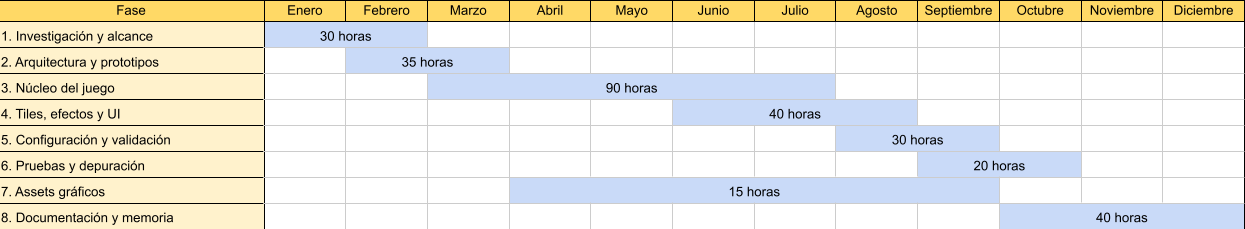
\includegraphics[width=0.95\textwidth]{Figuras/cronograma.png}
\caption{Diagrama de Gantt con la distribución temporal y la dedicación en horas de las ocho fases del proyecto (elaboración propia).}
\label{fig:gantt-planificacion}
\end{center}
\end{figure}


\section{Estructura de la memoria}


Esta memoria se organiza en seis capítulos. Tras la introducción, se analiza el estado del arte, referentes y tecnologías empleadas. Posteriormente, se detalla el diseño del sistema (requisitos y arquitectura) y su implementación técnica. Finalmente, se exponen las conclusiones y líneas de trabajo futuro.

\chapter{Estado del arte}

Este capítulo contextualiza el desarrollo de \textit{Ascension} mediante cuatro bloques: definición y relevancia del género \textit{roguelike}, análisis de referentes del mercado, justificación de las herramientas tecnológicas 2D seleccionadas y exposición de los patrones de diseño implementados.


\section{El subgénero \textit{roguelike}: definición y características}


\subsection{Origen histórico y evolución}


El término \textit{roguelike} tiene su origen en el videojuego \textit{Rogue}, desarrollado originalmente para sistemas Unix por Michael C. Toy, Glenn Wichman y Ken Arnold \cite{FREEBSD_ROGUE_MANPAGE}. Este juego introducía dos mecánicas que resultarían fundacionales para todo un subgénero: la generación procedural de niveles -- de modo que cada partida presentaba una disposición espacial diferente -- y la muerte permanente (\textit{permadeath}), que obligaba al jugador a reiniciar la partida desde el principio al perder todos los puntos de vida.

\begin{figure}[H]
\begin{center}
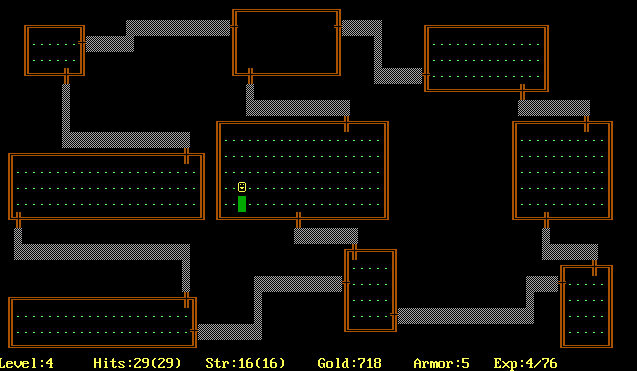
\includegraphics[width=0.9\textwidth]{Figuras/captura_3.png}
\caption{Captura de pantalla del videojuego original \textit{Rogue} (1980), mostrando la interfaz basada en caracteres ASCII y la disposición procedural de las salas. \textit{Fuente: captura histórica del juego.}}
\label{fig:placeholder-1}
\end{center}
\end{figure}


A lo largo de las décadas siguientes, numerosos títulos adoptaron y expandieron estas mecánicas. Juegos como \textit{NetHack} (1987), \textit{Angband} (1990) y \textit{Dungeon Crawl Stone Soup} (2006) mantuvieron la esencia del \textit{roguelike} clásico, caracterizado por gráficos basados en caracteres ASCII, mecánicas por turnos y una dificultad elevada. Sin embargo, a partir de la década de 2010, el subgénero experimentó una transformación significativa con la aparición de los denominados \textit{roguelites}, que incorporaban elementos del \textit{roguelike} clásico -- generación procedural y muerte permanente -- en combinación con mecánicas de acción en tiempo real, progresión entre partidas y diseño visual contemporáneo.

\subsection{Características técnicas fundamentales}


La comunidad de desarrolladores y jugadores ha intentado establecer criterios formales para definir qué constituye un \textit{roguelike}. La denominada \textit{Interpretación de Berlín} (International Roguelike Development Conference, 2008) \cite{BERLIN_INTERPRETATION} identificó las siguientes características como definitorias del subgénero:

\begin{enumerate}
\item \textbf{Generación procedural de niveles.} La estructura espacial del juego se genera algorítmicamente en cada partida, de modo que no existen dos ejecuciones idénticas. Esta característica implica la necesidad de diseñar algoritmos capaces de producir entornos jugables, coherentes y equilibrados sin intervención manual.
\item \textbf{Muerte permanente (\textit{permadeath}).} Al perder todos los puntos de vida, la partida finaliza de forma definitiva y el jugador debe reiniciar desde el principio. No existe la posibilidad de guardar y cargar el progreso del juego, lo que confiere a cada decisión del jugador un peso significativo.
\item \textbf{Progresión limitada a cada ejecución (\textit{run}, una partida completa desde el inicio hasta la muerte o victoria del jugador).} Las mejoras, armas y habilidades obtenidas durante una partida se pierden al morir. Cada ejecución comienza desde un estado inicial predefinido, aunque títulos más recientes (\textit{roguelites}) introducen sistemas de progresión permanente entre partidas.
\item \textbf{Sistema basado en turnos.} En la definición clásica, el jugador y los enemigos actúan de forma alternada. Sin embargo, los \textit{roguelikes} modernos y los \textit{roguelites} frecuentemente adoptan mecánicas de acción en tiempo real, como ocurre en el caso del proyecto \textit{Ascension}.
\item \textbf{Exploración de mazmorras (\textit{dungeon crawling}).} El jugador explora una sucesión de niveles o salas, enfrentándose a enemigos y recogiendo recursos, con el objetivo de alcanzar una condición de victoria definida.
\item \textbf{Alta rejugabilidad.} La combinación de generación procedural y la variabilidad de los elementos de juego (enemigos, objetos, disposición espacial) contribuye a que cada partida ofrezca una experiencia diferente, incentivando al jugador a repetir la experiencia.
\item \textbf{Complejidad de sistemas interconectados.} Los \textit{roguelikes} suelen presentar múltiples sistemas que interactúan entre sí de formas emergentes, generando situaciones impredecibles que enriquecen la experiencia de juego.
\end{enumerate}

\subsection{Importancia del género en la industria del videojuego}


El subgénero \textit{roguelike} ha experimentado un crecimiento notable en la última década, consolidándose como uno de los géneros más populares en el segmento de los videojuegos independientes. La amplia presencia de títulos etiquetados como \textit{roguelike} en catálogos de distribución digital refleja esta popularidad.

La relevancia del género se manifiesta en varios indicadores:

\begin{itemize}
\item \textbf{Éxito comercial.} Diversos títulos del subgénero han alcanzado un rendimiento comercial significativo, consolidándose como referencias dentro del mercado independiente.
\item \textbf{Reconocimiento crítico.} \textit{Hades} obtuvo reconocimiento en premios de la industria, incluyendo el premio al Mejor Juego Independiente en \textit{The Game Awards} 2020 \cite{CNET_GAME_AWARDS_2020_WINNERS}. Estos reconocimientos evidencian que el subgénero ha trascendido el ámbito de los juegos independientes para competir con producciones de mayor presupuesto.
\item \textbf{Influencia en el diseño de juegos.} Elementos propios del \textit{roguelike} -- generación procedural, \textit{permadeath}, rejugabilidad -- se han integrado en géneros distintos, dando lugar a híbridos como \textit{Returnal} (Housemarque, 2021), un juego de acción en tercera persona con estructura \textit{roguelike}, o \textit{Slay the Spire} (Mega Crit, 2019), que combina la estructura \textit{roguelike} con mecánicas de juegos de cartas \cite{STEAM_SLAY_THE_SPIRE_STORE}.
\item \textbf{Accesibilidad para desarrolladores independientes.} La generación procedural de contenido reduce la necesidad de diseño manual de niveles, lo que permite a equipos pequeños o desarrolladores individuales crear productos con una cantidad de contenido que, de otro modo, requeriría recursos significativamente mayores. Esta característica convierte al subgénero en un dominio adecuado para proyectos académicos como el presente Trabajo de Fin de Grado.
\end{itemize}

\begin{figure}[H]
\begin{center}
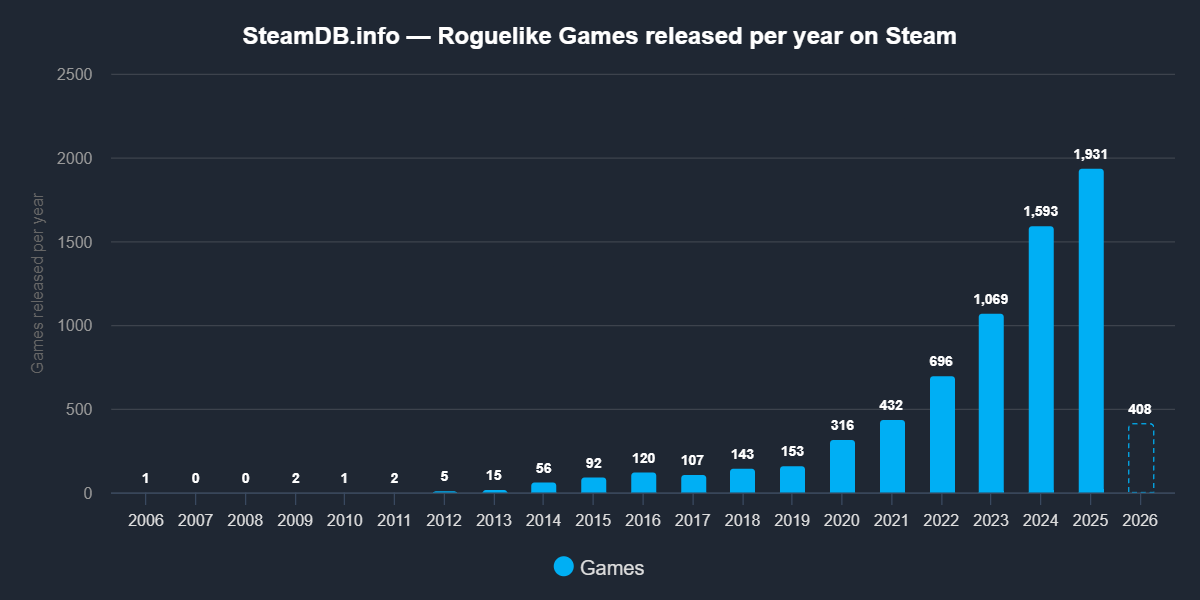
\includegraphics[width=0.9\textwidth]{Figuras/captura_4.png}
\caption{Gráfico que muestra la evolución del número de títulos \textit{roguelike} publicados en Steam por año (2006–2026). \textit{Fuente: SteamDB}}
\label{fig:placeholder-2}
\end{center}
\end{figure}


\subsection{Distinción entre \textit{roguelike} y \textit{roguelite}}


Resulta pertinente distinguir entre \textit{roguelike} en sentido estricto y \textit{roguelite}, dado que el proyecto \textit{Ascension} se sitúa en la intersección de ambas categorías:

\begin{table}[H]
\begin{center}
\small
\begin{tabular}{|p{0.307\textwidth}|p{0.307\textwidth}|p{0.307\textwidth}|}
\hline
\textbf{Característica} & \textbf{\textit{Roguelike} clásico} & \textbf{\textit{Roguelite}} \\ \hline
Generación procedural & Sí & Sí \\ \hline
Muerte permanente & Total & Total o parcial \\ \hline
Mecánica de combate & Por turnos & Tiempo real \\ \hline
Progresión entre partidas & No & Frecuente \\ \hline
Representación gráfica & ASCII o 2D simple & 2D/3D variada \\ \hline
Complejidad de sistemas & Muy alta & Moderada-alta \\ \hline
\end{tabular}
\end{center}
\end{table}


\TablaTitulo{Comparativa entre \textit{roguelike} clásico y \textit{roguelite}.}

\textit{Ascension} adopta las mecánicas fundamentales del \textit{roguelike} (generación procedural, \textit{permadeath}, exploración de mazmorras) con un sistema de combate en tiempo real propio del \textit{roguelite}, sin incluir progresión permanente entre partidas -- salvo la persistencia de puntuaciones -- lo que lo acerca más a la definición clásica del subgénero.

\subsection{Generación procedural de contenido}


La Generación Procedural de Contenido (GPC) constituye un conjunto de técnicas orientadas a la creación automática de datos de juego mediante algoritmos, reduciendo o eliminando la necesidad de diseño manual de niveles, escenarios o elementos del entorno (Shaker, Togelius y Nelson, 2016) \cite{SHAKER_PCG}.

En el contexto de los \textit{roguelikes}, la GPC resulta un componente central, ya que permite ofrecer variabilidad estructural y funcional en cada partida.

Entre los enfoques más utilizados para la generación procedural de niveles en videojuegos bidimensionales se encuentran:

\begin{itemize}
\item \textbf{Algoritmos basados en reglas.} Definen un conjunto de restricciones que deben cumplirse en el contenido generado (por ejemplo, que toda sala tenga al menos una salida accesible). El generador aplica estas reglas de forma iterativa hasta producir un resultado válido.
\item \textbf{Autómatas celulares.} Utilizados frecuentemente para la generación de cuevas orgánicas. Cada celda de una rejilla se evalúa según las celdas vecinas, produciendo formaciones naturales mediante iteraciones sucesivas.
\item \textbf{BSP (\textit{Binary Space Partitioning}).} Divide recursivamente el espacio disponible en subespacios menores, creando en cada subdivisión una habitación. Las habitaciones se conectan mediante pasillos, lo que genera estructuras de mazmorra clásicas.
\item \textbf{Sistemas deterministas con semillas pseudoaleatorias.} Utilizan un valor de semilla para inicializar el generador de números aleatorios, permitiendo reproducir exactamente la misma disposición espacial a partir de la misma semilla.
\item \textbf{Sistemas basados en \textit{Wave Function Collapse} (WFC).} Inspirados en la mecánica cuántica, definen restricciones de adyacencia entre tiles y resuelven iterativamente la disposición completa del nivel, produciendo resultados visualmente coherentes.
\item \textbf{Gramáticas formales y L-systems.} Utilizan reglas de producción para generar estructuras complejas a partir de axiomas simples, aplicados habitualmente a la generación de vegetación y elementos orgánicos.
\end{itemize}

En el caso de \textit{Ascension}, la generación procedural se basa en un enfoque híbrido: se utiliza una estructura rectangular fija de $26 \times 12$ tiles con bordes de muros perimetrales de un tile de grosor, sobre la cual se aplica un algoritmo de distribución aleatoria de tiles de suelo con variantes visuales y un algoritmo de expansión por \textit{clusters} para la colocación de tiles especiales con efectos.

La elección de este enfoque frente a técnicas más complejas como BSP o WFC se justifica por tres razones concretas. En primer lugar, la estructura rectangular fija simplifica el cálculo de posiciones válidas para la aparición de enemigos, ya que cualquier coordenada dentro del perímetro de muros constituye una posición válida sin necesidad de verificaciones adicionales de accesibilidad. En segundo lugar, los bordes perimetrales de muros impiden que el jugador pueda abandonar el área de juego sin necesidad de lógica de contención adicional; el colisionador del \textit{tilemap} de muros se genera automáticamente a partir de la posición de los tiles. En tercer lugar, el algoritmo de \textit{clusters} permite controlar la distribución espacial de los tiles especiales -- agrupándolos en manchas de entre cuatro y nueve tiles -- de forma que el jugador encuentre zonas con efectos lo suficientemente grandes como para influir en las decisiones tácticas de combate, pero no tan extensas como para dominar la sala. Este enfoque combina la previsibilidad estructural con la variabilidad de contenido que caracteriza al subgénero.

\subsubsection{Técnicas emergentes y trabajos recientes}


Además de los enfoques clásicos enumerados anteriormente, en los últimos años han surgido técnicas que amplían las posibilidades de la generación procedural en videojuegos:

\begin{itemize}
\item \textbf{Generación basada en restricciones con \textit{solvers} (Constraint Satisfaction Problems, CSP).} Formulan la generación de niveles como un problema de satisfacción de restricciones y emplean \textit{solvers} (como SAT o programación por restricciones) para encontrar configuraciones válidas que cumplan todas las condiciones impuestas. Smith y Mateas (2011) aplicaron esta técnica a la generación de niveles de plataformas 2D \cite{SMITH_MATEAS_2011}.
\item \textbf{Generación asistida por aprendizaje automático.} Se han explorado redes neuronales generativas (GANs -- \textit{Generative Adversarial Networks}) y autoencoders variacionales (VAEs -- \textit{Variational AutoEncoders}) para aprender la distribución de niveles diseñados manualmente y generar nuevos niveles consistentes con ese estilo (Volz et al., 2018) \cite{VOLZ_2018}.
\item \textbf{Funciones de ruido para generación de terreno.} Las funciones de ruido Perlin y Simplex, originalmente propuestas para la generación de texturas (Perlin, 1985) \cite{PERLIN_1985}, se utilizan ampliamente en juegos como \textit{Minecraft} y \textit{Terraria} para generar terrenos con apariencia natural.
\item \textbf{\textit{Wave Function Collapse} (WFC) aplicado a \textit{tilemaps}.} Gumin (2016) propuso el algoritmo WFC como un procedimiento genérico de generación a partir de ejemplos \cite{GUMIN_WFC_2016}. Karth y Smith (2017) analizaron formalmente el algoritmo y demostraron su equivalencia con ciertos modelos de propagación de restricciones \cite{KARTH_SMITH_2017}.
\end{itemize}

La siguiente tabla sintetiza la comparación entre las técnicas de generación procedural evaluadas y el enfoque adoptado en \textit{Ascension}:

\begin{table}[H]
\begin{center}
\small
\begin{tabular}{|p{0.23\textwidth}|p{0.23\textwidth}|p{0.23\textwidth}|p{0.23\textwidth}|}
\hline
\textbf{Técnica} & \textbf{Fortaleza principal} & \textbf{Limitación principal} & \textbf{Adecuación para \textit{Ascension}} \\ \hline
BSP & Salas irregulares con pasillos & Requiere verificación de accesibilidad & Baja: complejidad innecesaria para sala única \\ \hline
Autómatas celulares & Formas orgánicas (cuevas) & Difícil control de proporciones & Baja: salas rectangulares requeridas \\ \hline
WFC & Coherencia visual automática & Coste variable, reglas de adyacencia complejas & Moderada: sobrecomplejo para 8 tipos de tile \\ \hline
CSP / \textit{solvers} & Garantía de validez & Tiempo de cómputo elevado & Baja: no requiere verificación formal \\ \hline
GANs / VAEs & Captura de estilos implícitos & Requiere datos de entrenamiento, sin garantía & Baja: sin corpus de niveles previo \\ \hline
Ruido Perlin/Simplex & Terrenos naturales continuos & No discreto, sin control de salas & Baja: generación por tiles, no continua \\ \hline
Rejilla fija + \textit{clusters} & Control total, posicionamiento simple & Geometría invariante & Alta: equilibrio complejidad/variabilidad \\ \hline
\end{tabular}
\end{center}
\end{table}


\TablaTitulo{Comparativa de técnicas de generación procedural y su adecuación al proyecto.}

La tabla evidencia que, para un proyecto con sala rectangular fija, tres tipos de enemigo y un sistema de tiles con efectos como fuente principal de variabilidad, las técnicas más sofisticadas habrían incrementado la complejidad de implementación sin producir un beneficio proporcional en la experiencia de juego. La variabilidad táctica de \textit{Ascension} reside en la composición de tiles con efectos y en la combinación de oleadas de enemigos, no en la forma geométrica de la sala.

\subsection{Inteligencia artificial en videojuegos 2D}


La Inteligencia Artificial (IA) en videojuegos bidimensionales se orienta al diseño de comportamientos creíbles y coherentes para los Personajes No Jugables (PNJ) (Millington y Funge, 2009) \cite{MILLINGTON_AI}.

Las técnicas más empleadas para la implementación de IA en videojuegos incluyen:

\begin{itemize}
\item \textbf{Máquinas de estados finitos (FSM).} Definen un conjunto discreto de estados posibles para un PNJ y las condiciones que provocan la transición entre estados. Son fáciles de implementar y de depurar, pero pueden resultar rígidas cuando el número de estados crece.
\item \textbf{Árboles de comportamiento (\textit{behavior trees}).} Estructuran la lógica de decisión en forma de árbol jerárquico, donde cada nodo representa una condición, una acción o una secuencia de acciones.
\item \textbf{Sistemas de decisión basados en reglas.} Evalúan un conjunto de condiciones y ejecutan la acción asociada a la regla de mayor prioridad que se cumpla.
\item \textbf{Navegación por mallas (\textit{navmesh}) y \textit{pathfinding}.} Algoritmos como A* o Dijkstra permiten calcular rutas óptimas entre dos puntos del nivel.
\item \textbf{Sistemas de utilidad (\textit{Utility AI}).} Evalúan numéricamente la utilidad de cada acción disponible en función del estado actual del mundo.
\item \textbf{\textit{Goal-Oriented Action Planning} (GOAP).} Los agentes definen objetivos y planifican secuencias de acciones para alcanzarlos. Orkin (2003) introdujo GOAP en \textit{F.E.A.R.} \cite{ORKIN_2003}.
\item \textbf{Aprendizaje por refuerzo.} Los agentes aprenden comportamientos óptimos mediante la maximización de una función de recompensa. Unity ML-Agents (Juliani et al., 2018) \cite{JULIANI_2018} proporciona un \textit{framework} -- un entorno de desarrollo con herramientas y bibliotecas predefinidas -- integrado para entrenar agentes mediante aprendizaje por refuerzo profundo (DRL, \textit{Deep Reinforcement Learning}).
\end{itemize}

En \textit{Ascension}, la inteligencia artificial de los enemigos se implementa mediante una combinación de máquinas de estados simples y sistemas de decisión basados en reglas, cuya justificación se detalla en la siguiente tabla comparativa:

\begin{table}[H]
\begin{center}
\small
\begin{tabular}{|p{0.17\textwidth}|p{0.17\textwidth}|p{0.17\textwidth}|p{0.17\textwidth}|p{0.17\textwidth}|}
\hline
\textbf{Técnica} & \textbf{Complejidad de implementación} & \textbf{Expresividad} & \textbf{Depurabilidad} & \textbf{Adecuación para 3 tipos de enemigo} \\ \hline
FSM & Baja & Moderada & Alta (estados discretos) & Alta \\ \hline
Árboles de comportamiento & Moderada & Alta & Moderada (nodos jerárquicos) & Moderada \\ \hline
Sistemas de utilidad & Moderada-alta & Alta & Baja (valores continuos) & Baja \\ \hline
GOAP & Alta & Muy alta & Baja (planes dinámicos) & Baja \\ \hline
Aprendizaje por refuerzo & Muy alta & Variable & Muy baja (caja negra) & Muy baja \\ \hline
\end{tabular}
\end{center}
\end{table}


\TablaTitulo{Comparativa de técnicas de IA para enemigos en videojuegos 2D.}

\subsection{Mecánicas de combate en \textit{roguelikes}}


El sistema de combate constituye una de las mecánicas centrales de los videojuegos \textit{roguelike} y \textit{roguelite}. Los enfoques más habituales incluyen:

\begin{itemize}
\item \textbf{Combate por turnos.} El jugador y los enemigos ejecutan acciones de forma alternada. Es el enfoque clásico del subgénero (\textit{Rogue}, \textit{NetHack}).
\item \textbf{Combate en tiempo real con \textit{hack and slash} (combate de acción basado en ataques cuerpo a cuerpo rápidos y encadenados).} El jugador controla el personaje en tiempo real, ejecutando ataques de forma continua. Ejemplos representativos incluyen \textit{Hades} y \textit{Dead Cells}.
\item \textbf{Combate en tiempo real con componente de disparos (\textit{top-down shooter}).} El jugador dispara proyectiles hacia los enemigos desde una perspectiva cenital. Títulos como \textit{The Binding of Isaac} y \textit{Enter the Gungeon} han popularizado este enfoque.
\item \textbf{Combate híbrido.} Combina armas cuerpo a cuerpo y a distancia, permitiendo al jugador alternar entre estilos según la situación. \textit{Ascension} adopta este enfoque, ofreciendo ambas modalidades de combate con mecánicas diferenciadas.
\end{itemize}

\section{Análisis de mercado: referencias comerciales del subgénero}


El diseño y desarrollo de \textit{Ascension} se ha llevado a cabo tomando como referencia una selección de títulos comerciales representativos del subgénero \textit{roguelike} y \textit{roguelite}. El estudio de estos productos ha permitido identificar mecánicas de juego, decisiones de diseño y patrones de interacción que han influido en la definición de los sistemas del proyecto. A continuación se analizan los títulos más relevantes.

\subsection{The Binding of Isaac (2011, Edmund McMillen)}


\textit{The Binding of Isaac} es un \textit{roguelike} con perspectiva cenital (\textit{top-down}) cuya mecánica de combate se basa en el disparo de proyectiles en las cuatro direcciones cardinales. El jugador explora una sucesión de salas generadas proceduralmente, enfrentándose a enemigos con patrones de movimiento y ataque variados.

\textbf{Características relevantes para \textit{Ascension}:}
\begin{itemize}
\item \textbf{Estructura de salas.} Cada sala constituye un espacio cerrado con enemigos que deben ser derrotados antes de poder avanzar. En \textit{The Binding of Isaac}, las puertas de la sala se cierran al entrar y se abren al completarla. En \textit{Ascension}, la progresión se representa mediante escaleras que se bloquean durante el combate y se habilitan al completar la sala.
\item \textbf{Vista cenital.} La perspectiva \textit{top-down} permite al jugador una visión completa de la sala, facilitando la planificación táctica del movimiento y el combate. \textit{Ascension} utiliza esta misma perspectiva.
\item \textbf{Variedad de enemigos.} Cada tipo de enemigo presenta un comportamiento diferenciado (persecución, disparo, movimiento errático), lo que obliga al jugador a adaptar su estrategia continuamente.
\item \textbf{Sistema de jefes periódicos.} Al final de cada piso, el jugador se enfrenta a un enemigo jefe con estadísticas superiores y mecánicas de ataque propias. \textit{Ascension} implementa un sistema análogo con jefes cada cinco salas.
\end{itemize}

\begin{figure}[htbp]
\begin{center}
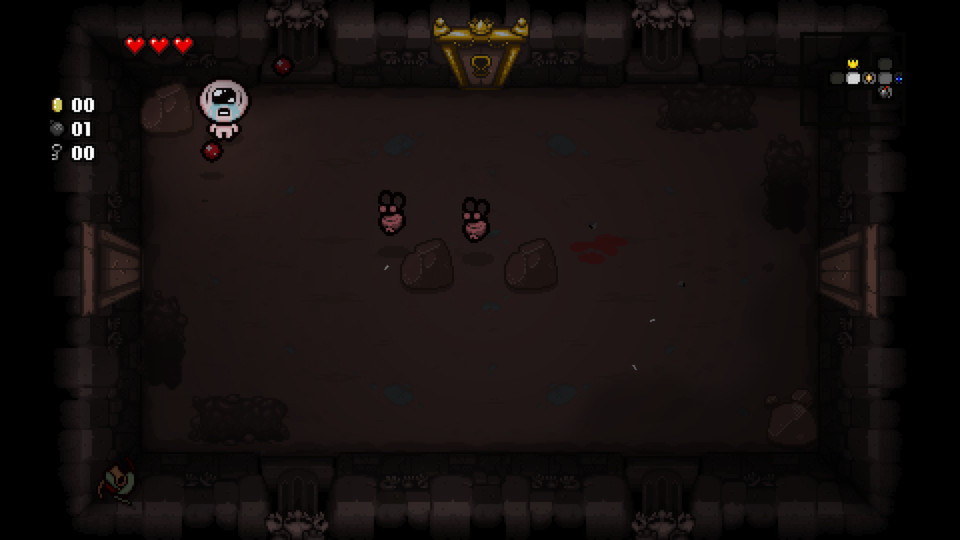
\includegraphics[width=0.9\textwidth]{Figuras/captura_5.png}
\caption{Captura de pantalla de \textit{The Binding of Isaac: Rebirth} en la que se observa la perspectiva cenital, la estructura de sala cerrada con puertas y la interfaz de vida mediante corazones en la esquina superior izquierda. \textit{Fuente: captura del juego en Steam.}}
\label{fig:placeholder-3}
\end{center}
\end{figure}


\subsection{Enter the Gungeon (2016, Dodge Roll)}


\textit{Enter the Gungeon} es un \textit{roguelite} cenital centrado en el combate con armas de fuego. Destaca por su sistema de esquiva (\textit{dodge roll}) y por la amplia variedad de armas disponibles, cada una con mecánicas diferenciadas.

\textbf{Características relevantes para \textit{Ascension}:}
\begin{itemize}
\item \textbf{Mecánica de esquiva (\textit{roll}).} El jugador puede ejecutar un movimiento rápido con invulnerabilidad temporal para evitar el daño de los proyectiles enemigos. \textit{Ascension} implementa una mecánica de esquiva equivalente, activada mediante la tecla Espacio, con un periodo de invulnerabilidad y un tiempo de espera entre usos.
\item \textbf{Combinación de combate a distancia y cuerpo a cuerpo.} \textit{Ascension} ofrece ambas modalidades de combate como mecánicas diferenciadas asociadas a tipos de arma distintos.
\item \textbf{Generación procedural con estructura por pisos.} El juego genera cada piso de la mazmorra de forma procedural. \textit{Ascension} adopta una estructura en la que se genera proceduralmente el contenido de la sala.
\end{itemize}

\begin{figure}[H]
\begin{center}
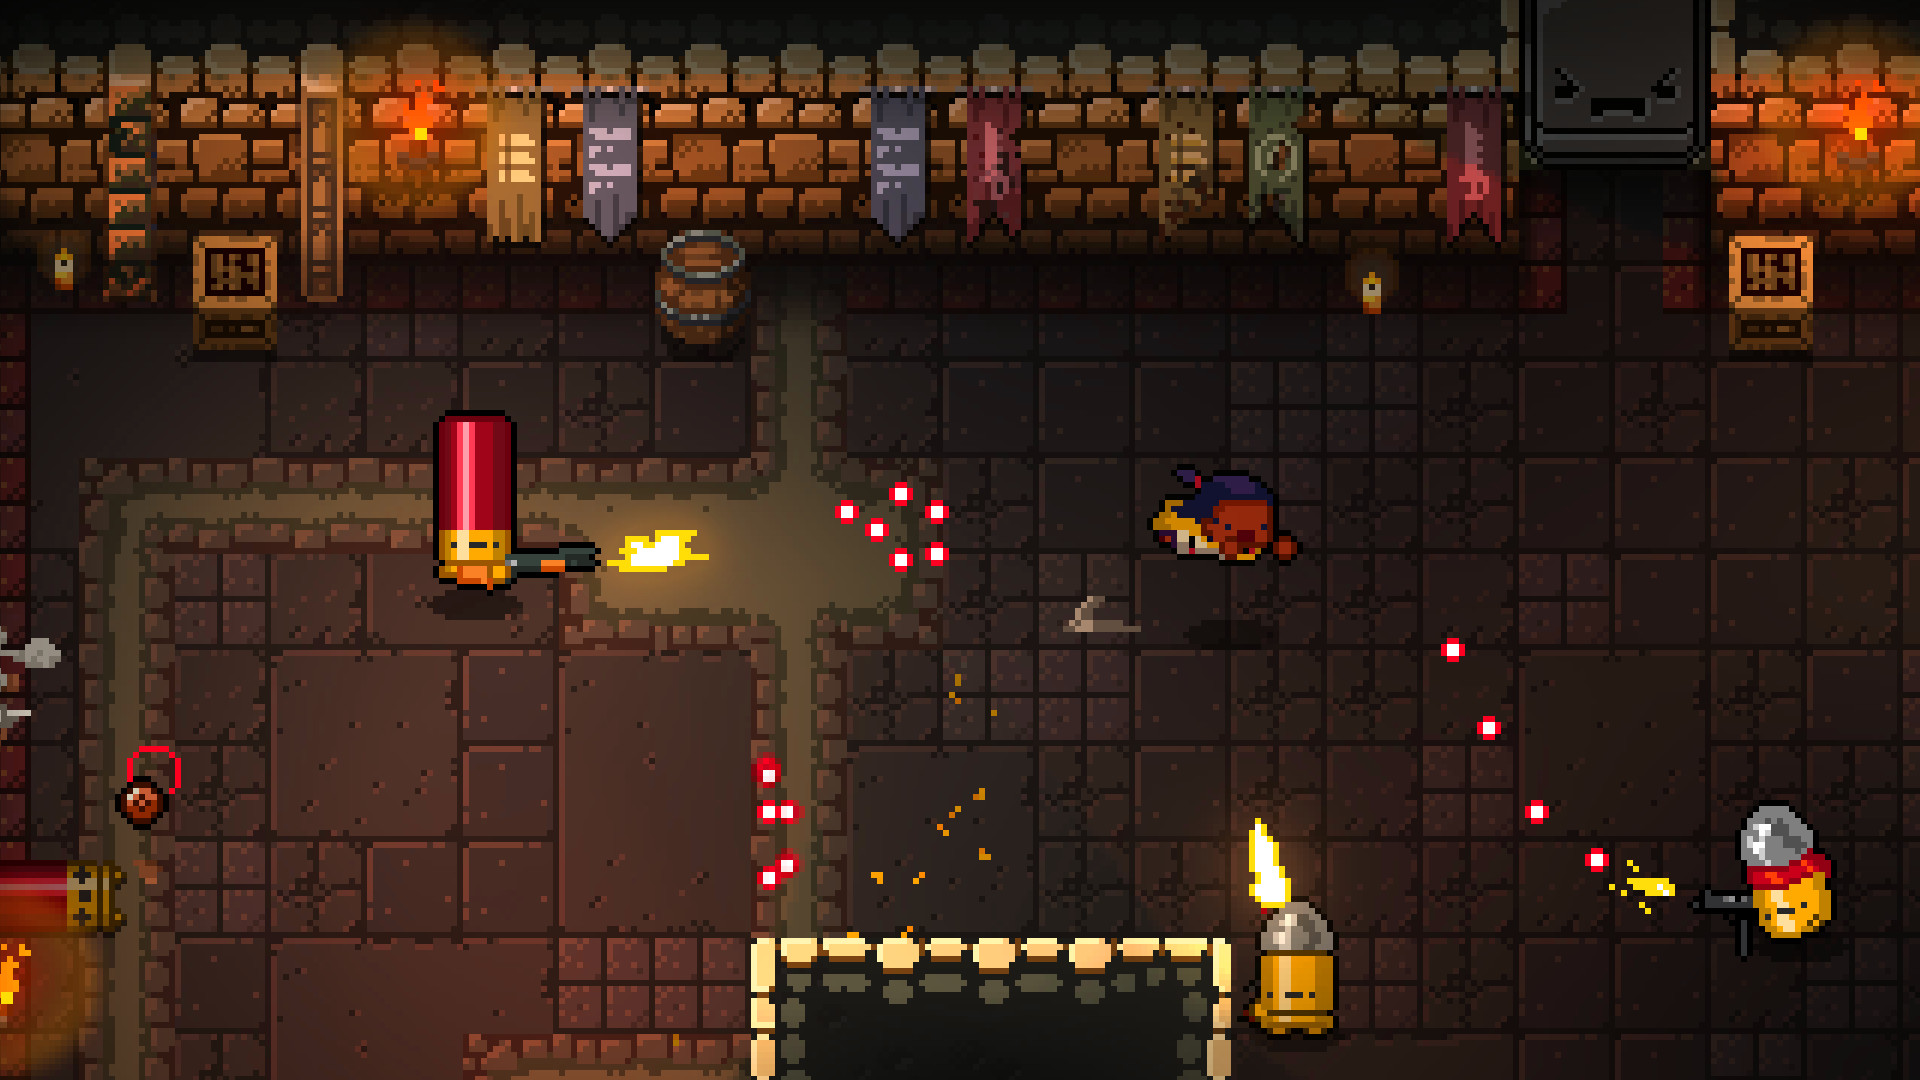
\includegraphics[width=0.9\textwidth]{Figuras/captura_6.png}
\caption{Captura de pantalla de \textit{Enter the Gungeon} en la que se muestra la mecánica de esquiva (\textit{dodge roll}) durante el combate y la variedad de proyectiles en pantalla. \textit{Fuente: captura del juego en Steam.}}
\label{fig:placeholder-4}
\end{center}
\end{figure}


\subsection{Hades (2020, Supergiant Games)}


\textit{Hades} es un \textit{roguelite} de acción con perspectiva isométrica que combina combate rápido con una narrativa progresiva. Ha recibido reconocimiento en premios de la industria; por ejemplo, en \textit{The Game Awards} 2020 obtuvo el galardón a Mejor Juego Independiente \cite{CNET_GAME_AWARDS_2020_WINNERS}.

\textbf{Características relevantes para \textit{Ascension}:}
\begin{itemize}
\item \textbf{Variedad de armas con mecánicas únicas.} Cada arma presenta un estilo de combate diferenciado (espada, arco, escudo, lanza). \textit{Ascension} implementa armas cuerpo a cuerpo y a distancia con mecánicas de ataque diferenciadas.
\item \textbf{Sistema de clases de personaje.} Aunque en \textit{Hades} no existen clases como tales, la selección de arma al inicio de cada ejecución determina el estilo de juego. \textit{Ascension} formaliza este concepto mediante un sistema de selección de clase con estadísticas diferenciadas.
\item \textbf{Enemigos con comportamientos variados.} Los enemigos presentan patrones de ataque diferenciados y coordinados. \textit{Ascension} implementa esta variedad mediante tres tipos de enemigos con comportamientos específicos.
\item \textbf{Retroalimentación visual del combate.} \textit{Hades} destaca por la retroalimentación visual que proporciona al jugador. \textit{Ascension} incorpora mecanismos análogos como el parpadeo en blanco del jugador al recibir daño y un parpadeo rojo rápido tanto en enemigos como en el jugador justo antes de morir.
\end{itemize}

\begin{figure}[H]
\begin{center}
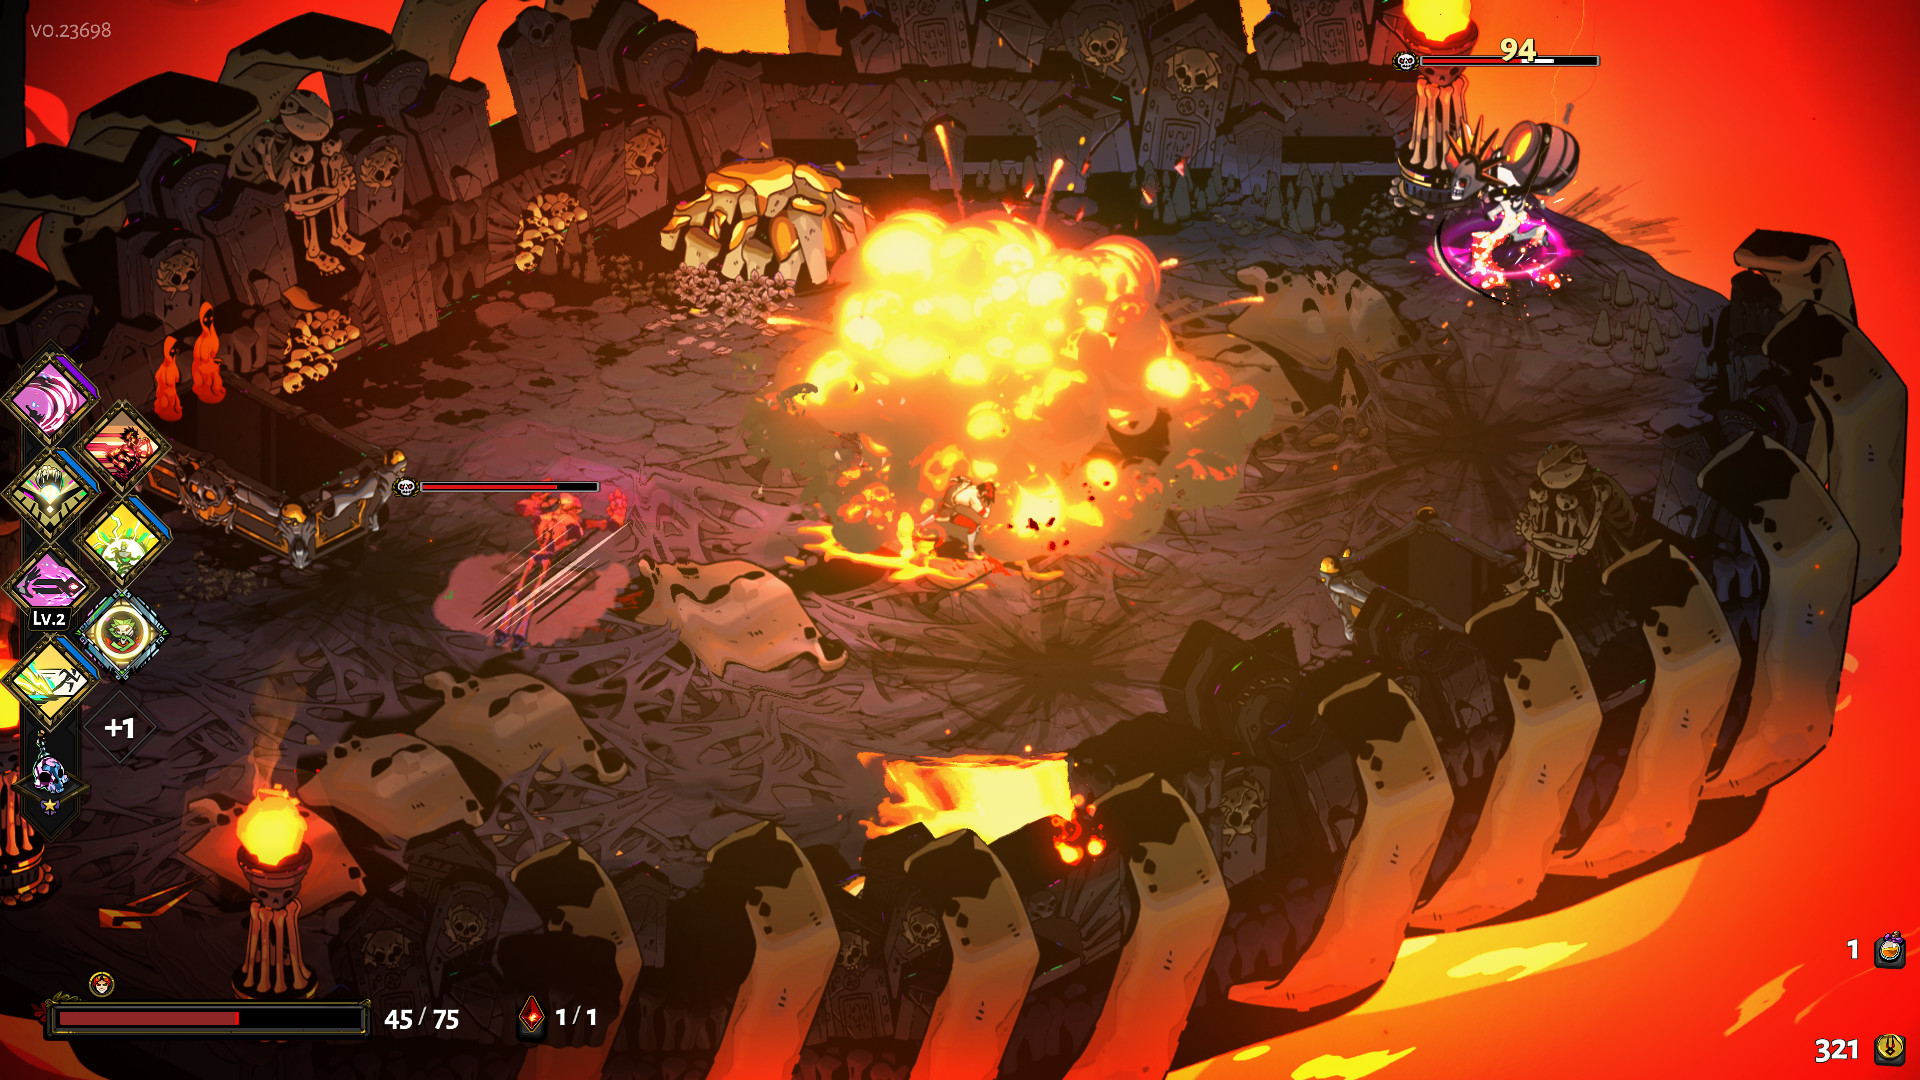
\includegraphics[width=0.9\textwidth]{Figuras/captura_7.png}
\caption{Captura de pantalla de \textit{Hades} en la que se aprecia el sistema de combate en tiempo real con arma cuerpo a cuerpo, la variedad de enemigos simultáneos y la interfaz de estado del personaje. \textit{Fuente: captura del juego en Steam.}}
\label{fig:placeholder-5}
\end{center}
\end{figure}


\subsection{Dead Cells (2018, Motion Twin)}


\textit{Dead Cells} es un \textit{roguelite} de acción lateral (\textit{side-scroller}) que combina exploración, combate fluido y un sistema de progresión permanente entre partidas.

\textbf{Características relevantes para \textit{Ascension}:}
\begin{itemize}
\item \textbf{Combate ágil y responsivo.} \textit{Dead Cells} se caracteriza por un combate rápido y preciso. En \textit{Ascension} se han implementado controles responsivos y tiempos de espera (\textit{cooldown}) reducidos con el objetivo de aproximarse a este enfoque.
\item \textbf{Armas con comportamientos diferenciados.} El juego ofrece una amplia variedad de armas cuerpo a cuerpo y a distancia. \textit{Ascension} implementa esta distinción mediante las clases \texttt{MeleeWeapon} y \texttt{RangedWeapon}, aplicando el patrón \textit{Strategy}.
\item \textbf{Escalonamiento de dificultad.} La dificultad aumenta de forma progresiva. En \textit{Ascension}, la dificultad se incrementa mediante el aumento del presupuesto de coste de enemigos por sala y la aparición periódica de enemigos especiales con atributos escalados.
\end{itemize}

En este contexto, el término \textit{cooldown} se refiere al \textbf{tiempo mínimo de espera entre dos ejecuciones de una misma acción} (por ejemplo, entre dos ataques consecutivos), y se utiliza como mecanismo de equilibrado para evitar acciones excesivamente frecuentes.

\begin{figure}[H]
\begin{center}
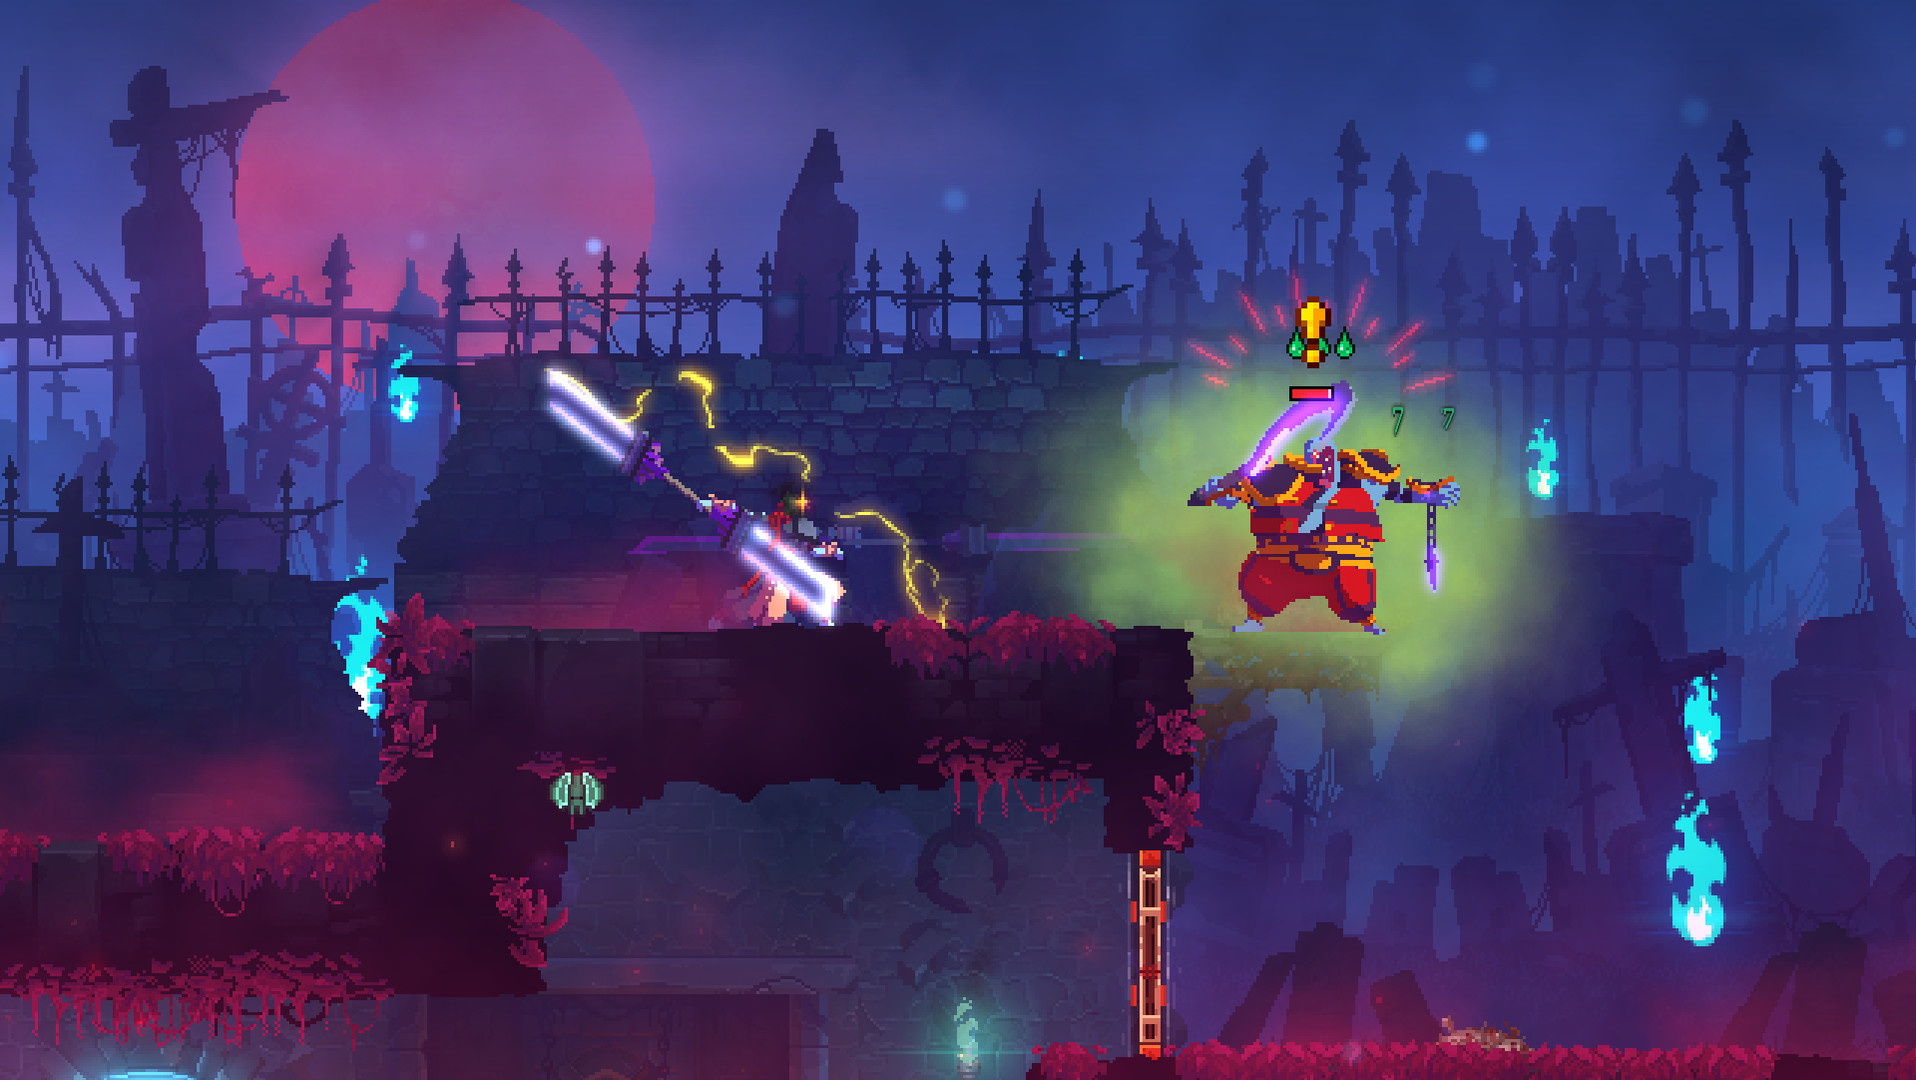
\includegraphics[width=0.9\textwidth]{Figuras/captura_8.png}
\caption{Captura de pantalla de \textit{Dead Cells} en la que se observa el combate lateral con armas cuerpo a cuerpo. \textit{Fuente: captura del juego en Steam.}}
\label{fig:placeholder-6}
\end{center}
\end{figure}


\subsection{Tabla comparativa de referencias comerciales}

La siguiente tabla compara las características de diseño y tecnología de los referentes analizados frente a \textit{Ascension}, justificando las decisiones adoptadas en cuanto a perspectiva, combate y mecánicas de movimiento.
\begin{table}[H]
\begin{center}
\small
\begin{tabular}{|p{0.153\textwidth}|p{0.153\textwidth}|p{0.153\textwidth}|p{0.153\textwidth}|p{0.153\textwidth}|p{0.153\textwidth}|}
\hline
Característica & The Binding of Isaac & Enter the Gungeon & Hades & Dead Cells & \textbf{Ascension} \\ \hline
Perspectiva & Cenital & Cenital & Isométrica & Lateral & \textbf{Cenital} \\ \hline
Generación procedural & Salas conectadas & Pisos con salas & Salas conectadas & Niveles laterales & \textbf{Salas secuenciales} \\ \hline
Combate & Disparo 4 direcciones & Disparo 360° + esquiva & Melee + distancia & Melee + distancia & \textbf{Melee + distancia} \\ \hline
Esquiva & No & \textit{Dodge roll} & \textit{Dash} & \textit{Roll} & \textbf{\textit{Roll} con invulnerabilidad} \\ \hline
Selección de personaje & Múltiples personajes & Múltiples personajes & Arma inicial & No & \textbf{3 clases con stats} \\ \hline
\textit{Permadeath} & Sí & Sí & Sí (con progresión) & Sí (con progresión) & \textbf{Sí} \\ \hline
Sistema de jefes & Final de piso & Final de piso & Final de zona & Por bioma & \textbf{Cada 5 salas} \\ \hline
Tiles con efectos & No & No & No & No & \textbf{Sí (hielo, lodo, curación, daño)} \\ \hline
Motor & Flash / C++ custom & Unity & Supergiant Engine & Custom & \textbf{Unity} \\ \hline
\end{tabular}
\end{center}
\end{table}


\TablaTitulo{Comparativa entre referencias comerciales y el proyecto \textit{Ascension}.}

\subsection{Elementos diferenciadores de \textit{Ascension}}


A partir del análisis comparativo anterior, es posible identificar los elementos que diferencian a \textit{Ascension} respecto a las referencias comerciales estudiadas:

\begin{enumerate}
\item \textbf{Sistema de tiles con efectos.} Ninguno de los títulos analizados incorpora un sistema de tiles especiales que modifiquen las condiciones de combate en tiempo real. Se incorporó este sistema en \textit{Ascension} para resolver un problema de diseño concreto: en un \textit{roguelike} con tres tipos de enemigo y un repertorio limitado de armas, la variabilidad táctica de cada sala depende exclusivamente de la composición de la oleada de enemigos, lo que puede generar repetitividad. Los tiles con efectos -- hielo (incremento de velocidad), lodo (reducción de velocidad), curación y potenciación de daño -- introducen una segunda dimensión de variabilidad: el entorno físico de la sala condiciona las decisiones tácticas del jugador. La alternativa descartada era añadir más tipos de enemigo, pero esto habría incrementado significativamente el volumen de arte y animación necesario.
\item \textbf{Arquitectura orientada a la extensibilidad.} Se adoptó la separación entre datos configurables (\textit{ScriptableObjects}) y lógica de juego como principio arquitectónico deliberado. Esta decisión responde a una necesidad práctica del desarrollo: los parámetros de configuración se modificaron en numerosas ocasiones. Con \textit{ScriptableObjects}, cada ajuste se realiza editando un campo numérico en el inspector, con efecto inmediato y sin recompilación. La implicación arquitectónica es que el sistema cumple el principio de apertura-cierre (\textit{Open-Closed Principle}) de los principios SOLID.
\end{enumerate}

\begin{figure}[H]
\begin{center}
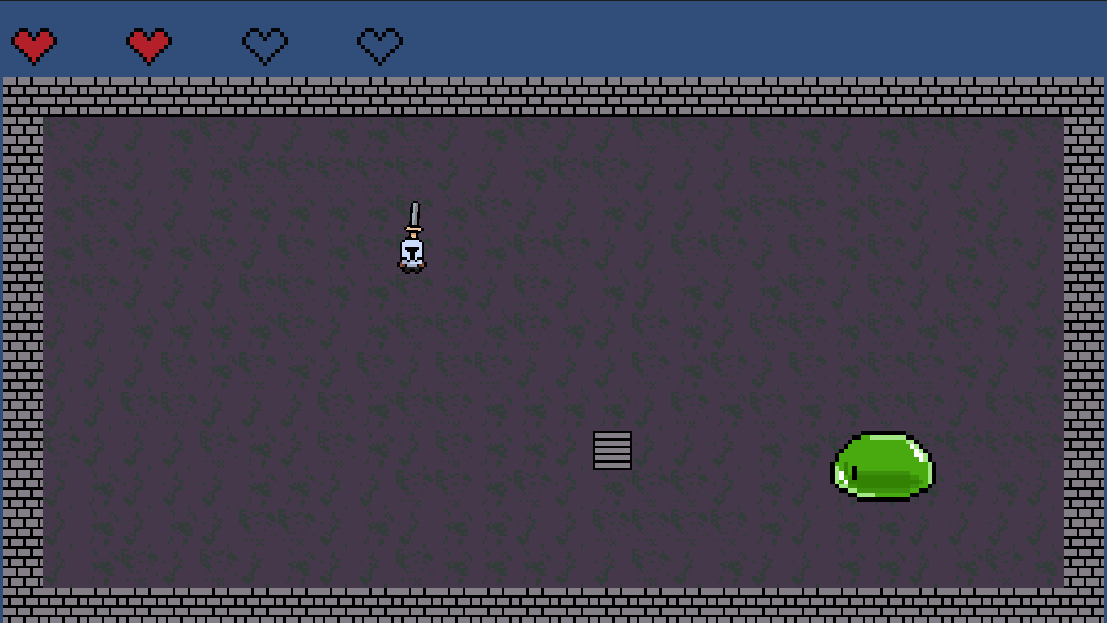
\includegraphics[width=0.9\textwidth]{Figuras/Jefe.png}
\caption{Captura de pantalla de \textit{Ascension} durante una partida, mostrando la perspectiva cenital, la sala generada proceduralmente con tiles especiales visibles (hielo, lodo), enemigos activos y la interfaz de corazones. \textit{Elaboración propia.}}
\label{fig:placeholder-7}
\end{center}
\end{figure}


\begin{figure}[H]
\begin{center}
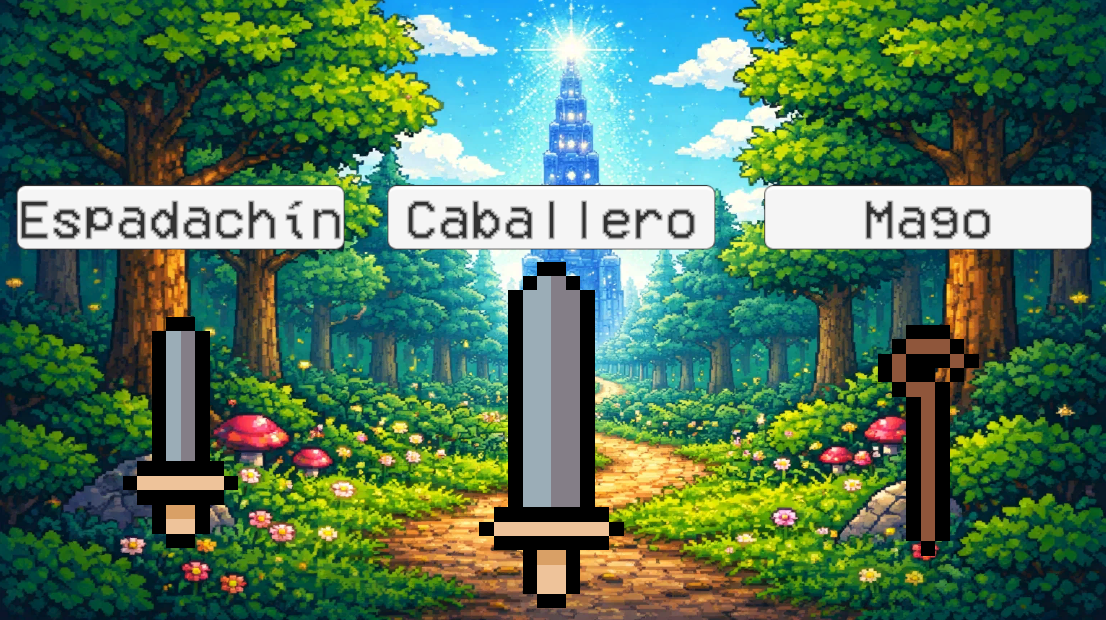
\includegraphics[width=0.9\textwidth]{Figuras/captura_1.png}
\caption{Captura de pantalla de \textit{Ascension} mostrando la pantalla de selección de clase. \textit{Elaboración propia.}}
\label{fig:placeholder-8}
\end{center}
\end{figure}




\section{Análisis de herramientas y tecnologías}


\subsection{Motores de desarrollo de videojuegos}


La selección del motor de desarrollo constituye una decisión técnica de gran relevancia en cualquier proyecto de videojuegos. A continuación se analizan los motores más relevantes para el desarrollo de videojuegos bidimensionales.

\subsubsection{Unity}


Unity es un motor de desarrollo multiplataforma creado por Unity Technologies en 2005. Constituye una de las herramientas más utilizadas en la industria; Unity indica que más del 70\% de los 1.000 juegos móviles más populares se desarrollaron con Unity (dato referido a Q4 2022 con fuente Apptopia) \cite{UNITY_MOBILE_TOP1000_APPTOPIA_Q4_2022}. Sus características principales incluyen:

\begin{itemize}
\item \textbf{Arquitectura basada en componentes (\textit{Entity-Component System}).} Las entidades del juego se definen como agregaciones de componentes reutilizables.
\item \textbf{Sistema de \textit{Tilemaps} integrado.} Proporciona herramientas nativas para la creación y gestión de niveles basados en tiles, incluyendo colisionadores automáticos.
\item \textbf{Lenguaje de programación C\#.} Ofrece tipado fuerte, soporte completo para programación orientada a objetos y acceso a la biblioteca estándar de .NET.
\item \textbf{Sistema de \textit{ScriptableObjects}.} Permite almacenar datos configurables como activos del proyecto.
\item \textbf{Soporte multiplataforma.} Permite compilar el proyecto para más de veinte plataformas.
\item \textbf{Comunidad y recursos.} Cuenta con documentación oficial detallada, foros activos y un amplio ecosistema de \textit{assets}.
\end{itemize}

\subsubsection{Godot Engine}


Godot es un motor de código abierto creado por Juan Linietsky y Ariel Manzur, publicado bajo licencia MIT. Sus características incluyen:

\begin{itemize}
\item \textbf{Arquitectura basada en nodos y escenas.} Toda entidad es un nodo dentro de un árbol de escenas.
\item \textbf{Lenguaje GDScript.} Lenguaje propio con sintaxis similar a Python. También soporta C\# y C++.
\item \textbf{Código abierto.} Permite acceder y modificar el código fuente del motor.
\item \textbf{Sistema de \textit{TileMap} y \textit{TileSet}.} Proporciona herramientas para el diseño de niveles 2D.
\item \textbf{Sin costes de licencia.}
\end{itemize}

\subsubsection{Unreal Engine}


Unreal Engine, desarrollado por Epic Games, es un motor enfocado principalmente en gráficos de alta fidelidad para juegos 3D AAA:

\begin{itemize}
\item \textbf{Sistema \textit{Blueprints}.} Permite programar mediante un sistema de scripting visual.
\item \textbf{Lenguaje C++.} Ofrece rendimiento nativo y control de bajo nivel.
\item \textbf{Orientación principal a 3D.} Carece de herramientas nativas específicas como \textit{tilemaps}.
\item \textbf{Peso del editor.} El editor tiene un tamaño considerable (más de 60 GB).
\end{itemize}

\subsubsection{GameMaker}


GameMaker, desarrollado por YoYo Games, es un motor orientado al desarrollo de videojuegos 2D:

\begin{itemize}
\item \textbf{Lenguaje GML (\textit{GameMaker Language}).} Orientado a la simplicidad.
\item \textbf{Especialización en 2D.} Herramientas nativas optimizadas para la creación de juegos bidimensionales.
\item \textbf{Limitaciones en proyectos complejos.} Arquitectura menos flexible para proyectos con requerimientos de modularidad avanzada.
\item \textbf{Licencia de pago.}
\end{itemize}

\subsection{Tabla comparativa de motores de desarrollo}

La elección del motor de desarrollo es un factor crítico para el éxito del proyecto. La siguiente tabla evalúa las alternativas más relevantes del mercado, comparando criterios técnicos clave —como el soporte nativo 2D y la gestión de datos— para justificar la idoneidad de la tecnología seleccionada para Ascension.

\begin{table}[H]
\begin{center}
\small
\begin{tabular}{|p{0.184\textwidth}|p{0.184\textwidth}|p{0.184\textwidth}|p{0.184\textwidth}|p{0.184\textwidth}|}
\hline
\textbf{Criterio} & \textbf{Unity} & \textbf{Godot} & \textbf{Unreal Engine} & \textbf{GameMaker} \\ \hline
Licencia & Gratuito (con restricciones) & MIT (libre) & Gratuito (regalías al 5 \%) & Pago \\ \hline
Lenguaje principal & C\# & GDScript / C\# & C++ / Blueprints & GML \\ \hline
Soporte 2D nativo & Excelente & Bueno & Limitado & Excelente \\ \hline
Sistema de \textit{Tilemaps} & Integrado y maduro & Integrado (Godot 4) & No nativo & Integrado \\ \hline
\textit{ScriptableObjects} & Sí & Recursos equivalentes & \textit{Data Assets} & No \\ \hline
Documentación y comunidad & Muy amplia & Creciente & Amplia (centrada en 3D) & Moderada \\ \hline
Soporte multiplataforma & +20 plataformas & +10 plataformas & +10 plataformas & +10 plataformas \\ \hline
Curva de aprendizaje & Moderada & Baja-moderada & Alta & Baja \\ \hline
Idoneidad para \textit{roguelikes} 2D & Alta & Alta & Baja & Moderada \\ \hline
\end{tabular}
\end{center}
\end{table}


\TablaTitulo{Comparativa de motores de desarrollo de videojuegos.}

\subsection{Justificación de la elección de Unity y C\#}


Se seleccionó Unity frente a Godot, Unreal Engine y GameMaker tras evaluar los criterios recogidos en la Tabla 2.5. La decisión se basa en cuatro requisitos técnicos concretos del proyecto:

\begin{enumerate}
\item \textbf{Madurez del sistema de \textit{Tilemaps}.} La generación procedural de salas basada en \textit{tilemaps} constituye una funcionalidad central del proyecto. El componente \texttt{TilemapCollider2D} de Unity genera colisionadores de forma nativa a partir de la disposición de tiles, mientras que en Godot la creación de colisionadores por tile requería configuración manual adicional.
\item \textbf{Sistema de \textit{ScriptableObjects}.} Resuelve un problema arquitectónico concreto: la separación entre datos configurables y lógica de ejecución. Sin este mecanismo, ajustar un parámetro de equilibrado obligaría a recompilar el proyecto.
\item \textbf{Lenguaje C\#.} Ofrece tipado fuerte, soporte completo para programación orientada a objetos (herencia, polimorfismo, interfaces), manejo de excepciones, eventos y delegados. Estas características resultan fundamentales para la implementación de patrones de diseño como \textit{Singleton}, \textit{Observer} y \textit{Strategy}.
\item \textbf{Documentación y soporte.} La documentación oficial de Unity, los foros de la comunidad y la abundancia de recursos formativos facilitan la resolución de problemas técnicos de forma autónoma.
\end{enumerate}

\subsection{Correspondencia entre funcionalidades de Unity/C\# y subsistemas del proyecto}


La implementación de los subsistemas en Ascension depende de características específicas del motor y del lenguaje C\#. La siguiente tabla detalla estas funcionalidades y su equivalencia en motores alternativos, permitiendo comprender cómo la arquitectura del proyecto -- basada en patrones como Observer o Strategy -- se ve favorecida por las herramientas nativas de Unity.


\begin{table}[H]
\begin{center}
\scriptsize
\setlength{\tabcolsep}{2pt}
\begin{tabular}{|p{0.22\textwidth}|p{0.155\textwidth}|p{0.155\textwidth}|p{0.155\textwidth}|p{0.155\textwidth}|}
\hline
\textbf{Funcionalidad de Unity / C\#} & \textbf{Subsistema que la utiliza} & \textbf{Godot} & \textbf{Unreal} & \textbf{GameMaker} \\ \hline
\texttt{TilemapCollider2D}\newline(colisionadores automáticos) & Generación procedural de salas (\texttt{RoomGenerator}) & Requiere config. manual por tile & No nativo para 2D & No aplicable \\ \hline
\texttt{CompositeCollider2D}\newline(fusión de colisionadores) & Bordes perimetrales de sala & Equivalente parcial & No nativo para 2D & No aplicable \\ \hline
\texttt{ScriptableObject} +\newline\texttt{[CreateAssetMenu]} & Datos de enemigos, armas, clases, tiles & \texttt{Resource} (menor integración) & \texttt{Data Asset} (requiere C++) & No disponible \\ \hline
Delegados y eventos (\texttt{event Action<T>}) & Patrón \textit{Observer} en \texttt{GameManager} & Señales (\textit{signals}) & Delegados multicast (C++) & No disponible \\ \hline
Herencia + \texttt{virtual} / \texttt{override} & Patrón \textit{Template Method} (enemigos), \textit{Strategy} (armas) & Herencia con \texttt{extends} & Herencia en C++ & No soporta herencia \\ \hline
Corutinas (\texttt{IEnumerator} + \texttt{yield return}) & Invulnerabilidad, efectos temporales, espera & Equivalente (\texttt{await}) & Latent actions & Alarmas (limitadas) \\ \hline
\texttt{DontDestroyOnLoad} & Persistencia de \textit{Singletons} entre escenas & \texttt{autoload} & \texttt{GameInstance} & Objetos persistentes \\ \hline
\texttt{[SerializeField]} & Exposición de campos privados al inspector & \texttt{@export} & \texttt{UPROPERTY()} & No aplicable \\ \hline
\texttt{Physics2D.OverlapCircle} / \texttt{CompareTag} & Detección de colisiones e identificación de entidades & Áreas 2D + grupos & Canales de colisión (C++) & Colisiones simples \\ \hline
\end{tabular}
\end{center}
\end{table}


\TablaTitulo{Correspondencia entre funcionalidades de Unity/C\# utilizadas en el proyecto y sus equivalentes en motores alternativos.}

\subsection{Otras herramientas utilizadas}


Además del motor de desarrollo, el proyecto ha contado con un ecosistema de herramientas auxiliares que optimizan la calidad del código, el control de versiones y el diseño visual. La siguiente tabla detalla este conjunto de herramientas y las razones técnicas de su selección.


\begin{table}[H]
\begin{center}
\small
\begin{tabular}{|p{0.307\textwidth}|p{0.307\textwidth}|p{0.307\textwidth}|}
\hline
\textbf{Herramienta} & \textbf{Propósito} & \textbf{Justificación} \\ \hline
Visual Studio & Entorno de desarrollo integrado (IDE) & Autocompletado inteligente para C\# y Unity, depuración integrada, refactorización \\ \hline
LibreSprite & Creación de \textit{pixel art} & Editor de sprites de código abierto con soporte para animaciones frame-by-frame \\ \hline
Git & Control de versiones & Seguimiento de cambios, gestión de ramas y recuperación de estados anteriores del proyecto \\ \hline
PlantUML & Diagramas UML (\textit{Unified Modeling Language}) & Generación de diagramas UML a partir de texto plano \\ \hline
TextMesh Pro (Unity) & Renderizado de texto en UI & Sistema de renderizado de texto de alta calidad integrado en Unity \\ \hline
\end{tabular}
\end{center}
\end{table}


\TablaTitulo{Herramientas complementarias utilizadas en el desarrollo.}

\subsubsection{LibreSprite: creación de sprites y animación en \textit{pixel art}}


En un videojuego 2D con estética \textit{pixel art}, la herramienta de creación gráfica condiciona directamente la calidad del resultado y la eficiencia del flujo de producción de activos. En \textit{Ascension}, LibreSprite se emplea para la elaboración de \textit{sprites} (personaje, enemigos, proyectiles y tiles) y para animaciones \textit{frame-by-frame}.

Para contextualizar su elección, la Tabla 2.8 compara LibreSprite con dos herramientas habituales en proyectos 2D:

\begin{table}[H]
\begin{center}
\small
\begin{tabular}{|p{0.21\textwidth}|p{0.21\textwidth}|p{0.21\textwidth}|p{0.21\textwidth}|}
\hline
\textbf{Criterio} & \textbf{LibreSprite} & \textbf{Aseprite} & \textbf{Figma} \\ \hline
Enfoque principal & \textit{Pixel art} y animación 2D & \textit{Pixel art} y animación 2D & Diseño UI/UX (vectorial) \\ \hline
Animación \textit{frame-by-frame} & Sí & Sí & Limitada (no orientada a sprites) \\ \hline
Control de píxel y paletas & Alto & Alto & Medio (depende de plugins/flujo) \\ \hline
Adecuación para sprites $16 \times 16$ / $32 \times 32$ & Alta & Alta & Baja-moderada \\ \hline
\end{tabular}
\end{center}
\end{table}


\TablaTitulo{Comparativa de herramientas para producción de gráficos 2D.}

Se seleccionó LibreSprite frente a Aseprite y Figma por dos razones concretas. En primer lugar, LibreSprite es \textit{software} de código abierto y licencia libre. En segundo lugar, Figma se descartó porque su enfoque vectorial no está diseñado para edición \textit{pixel-perfect} a resoluciones de $16 \times 16$ o $32 \times 32$ píxeles.

Desde el punto de vista de integración con el motor, el flujo de trabajo consiste en exportar los recursos desde LibreSprite en formato PNG (como sprites individuales o \textit{spritesheets}) e importarlos en Unity configurando parámetros de \textit{pixel art}: \texttt{Pixels Per Unit} coherente con el tamaño de tile (16), filtrado sin suavizado (\textit{Point}) y compresión desactivada para preservar la nitidez.

\begin{figure}[H]
\begin{center}
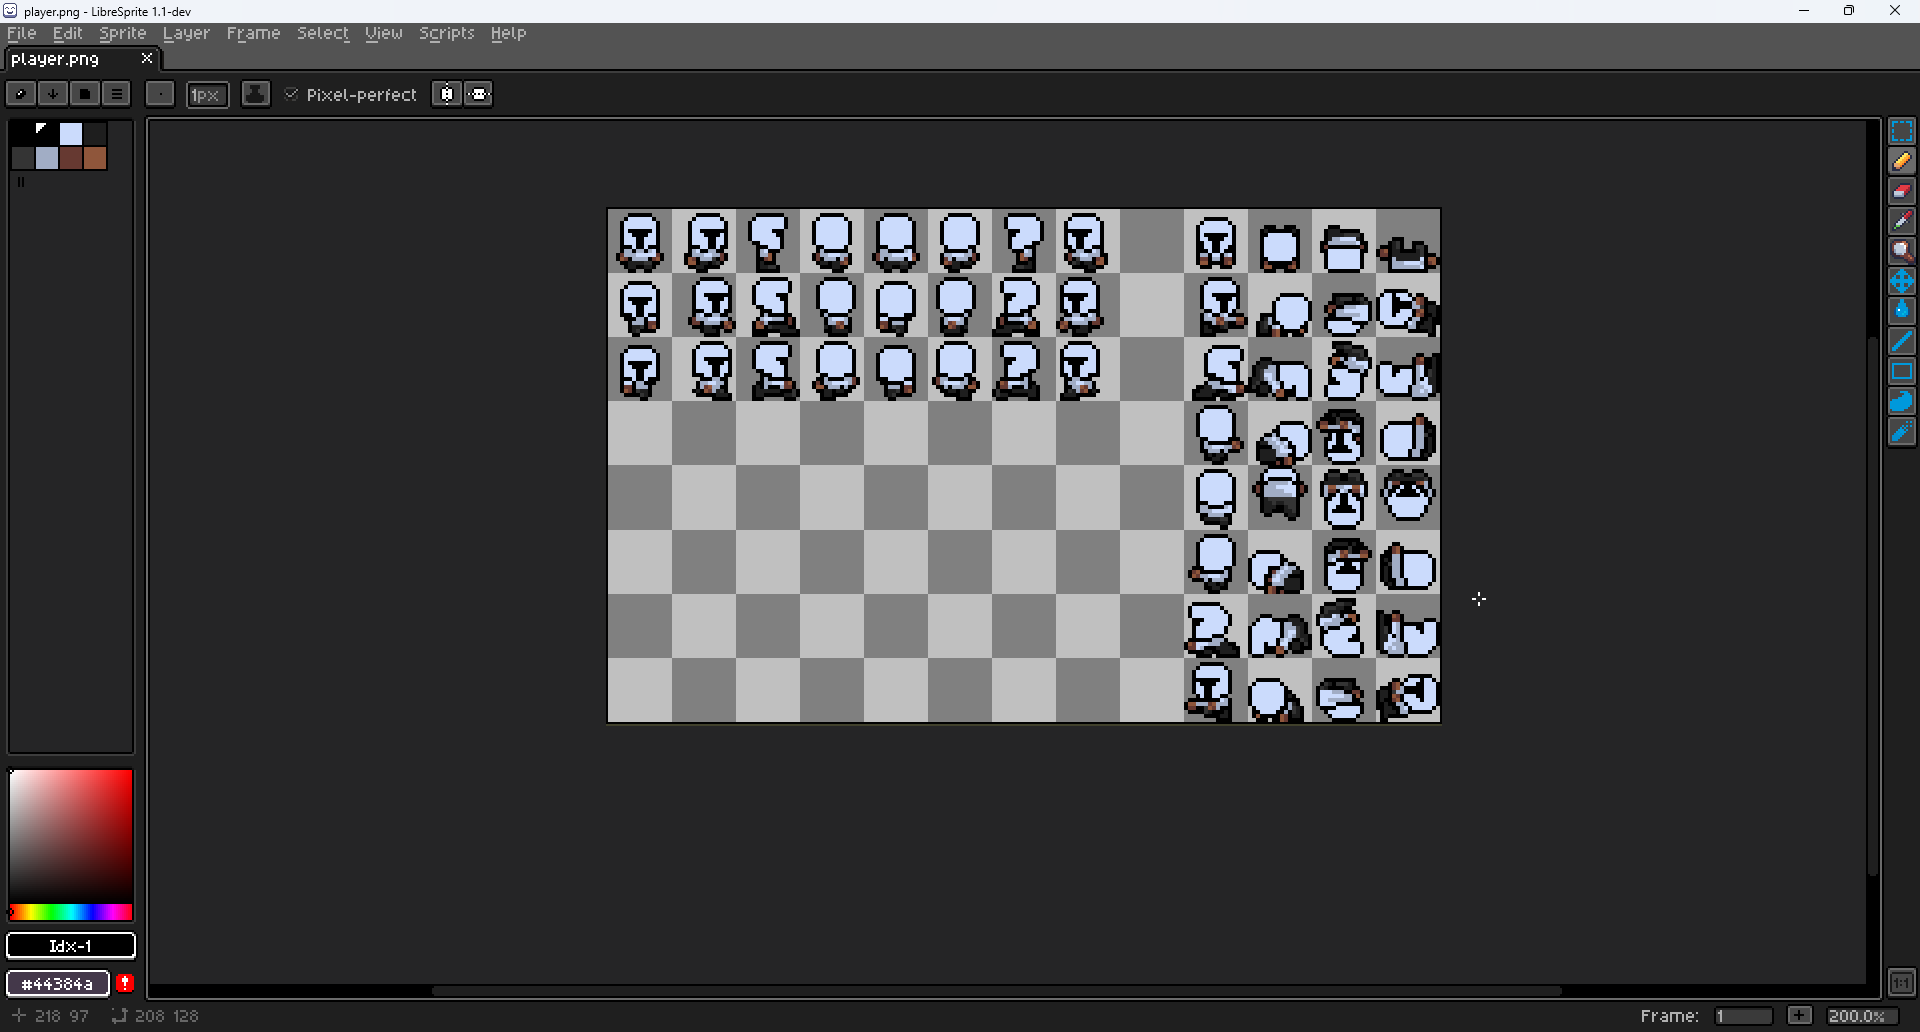
\includegraphics[width=0.9\textwidth]{Figuras/captura_2.png}
\caption{Captura de la interfaz de LibreSprite durante la edición de un \textit{sprite} del juego \textit{Ascension}, mostrando la paleta de colores y el lienzo de edición. \textit{Elaboración propia.}}
\label{fig:placeholder-9}
\end{center}
\end{figure}




\section{Patrones de diseño en el desarrollo de videojuegos}


El desarrollo de videojuegos de complejidad media-alta requiere la aplicación de patrones de diseño (Gamma et al., 1994) \cite{GAMMA_PATTERNS} que faciliten la organización del código, la separación de responsabilidades y la evolución del sistema. A continuación se describen los patrones más relevantes en este contexto, que se han aplicado en el desarrollo de \textit{Ascension}.

\subsection{Patrón \textit{Singleton}}


El patrón \textit{Singleton} establece que una clase disponga de una única instancia en toda la aplicación y proporciona un punto de acceso global a dicha instancia. Su uso implica un compromiso: simplifica el acceso a servicios globales pero introduce un acoplamiento implícito. Se seleccionó el patrón \textit{Singleton} frente a la inyección de dependencias por una razón práctica: en un proyecto individual con cuatro gestores centrales, la infraestructura de un contenedor de inyección de dependencias habría añadido complejidad sin beneficio proporcional. En \textit{Ascension}, se utiliza de forma controlada en los gestores centrales (\textit{GameManager}, \textit{ScoreManager}, \textit{RoomFlowController}, \textit{DamageBoostManager}), todos ellos persistentes entre escenas mediante \texttt{DontDestroyOnLoad}.

\subsection{Patrón \textit{Observer}}


El patrón \textit{Observer} define una relación de dependencia uno-a-muchos entre objetos. Se seleccionó este patrón frente a la alternativa directa -- que el \texttt{GameManager} invocara explícitamente métodos de cada componente de interfaz -- porque esta última habría creado una dependencia inversa que violaría el principio de inversión de dependencias. En \textit{Ascension}, el \textit{GameManager} expone eventos como \texttt{OnGameStateChanged}, \texttt{OnRoomCleared} y \texttt{OnEnemyKilled}, a los que se suscriben los componentes de interfaz de usuario y otros subsistemas.

\subsection{Patrón \textit{Strategy}}


El patrón \textit{Strategy} define una familia de algoritmos, encapsula cada uno de ellos y los hace intercambiables. Se seleccionó frente a la alternativa de una única clase \texttt{Weapon} con condicionales \texttt{if/else}. La clase base \texttt{Weapon} define la interfaz común (método \texttt{Attack()}), mientras que \texttt{MeleeWeapon} y \texttt{RangedWeapon} proporcionan implementaciones específicas. Esto permite añadir nuevos tipos de arma creando una nueva subclase sin modificar el código existente.

\subsection{Patrón \textit{Template Method}}


El patrón \textit{Template Method} define el esqueleto de un algoritmo en una operación, delegando en las subclases la definición de determinados pasos. En \textit{Ascension}, la clase base \texttt{Enemy}  define el ciclo de vida común de todos los enemigos, mientras que las subclases (\texttt{SlimeGreen}, \texttt{SlimeRed}, \texttt{SlimeBlue}) sobrescriben los métodos virtuales para definir su comportamiento específico de IA.

\subsection{Arquitectura basada en componentes (Entidad-Componente)}


Unity se fundamenta en una arquitectura basada en componentes, donde las entidades del juego (\textit{GameObjects}) se definen como contenedores vacíos a los que se agregan componentes (\textit{MonoBehaviour}) que encapsulan funcionalidades independientes. Esta arquitectura favorece la composición sobre la herencia.

\subsection{Máquina de estados (\textit{State Machine})}


Una máquina de estados define un conjunto finito de estados posibles y las transiciones válidas entre ellos. En \textit{Ascension}, el \textit{GameManager} implementa una máquina de estados que controla el flujo global del juego con los estados: \texttt{Menu}, \texttt{CharacterSelection}, \texttt{Playing}, \texttt{Paused}, \texttt{GameOver} y \texttt{Victory}.



\section{Síntesis del estado del arte}


El análisis realizado en este capítulo permite establecer las siguientes conclusiones:

\begin{enumerate}
\item El subgénero \textit{roguelike} presenta retos técnicos de considerable complejidad que justifican su abordaje en un Trabajo de Fin de Grado, incluyendo la generación procedural de contenido, la implementación de inteligencia artificial reactiva y la gestión de múltiples subsistemas en tiempo real. Su creciente relevancia en la industria del videojuego, tanto en términos comerciales como en reconocimiento crítico, refuerza la pertinencia de su estudio.
\item Los títulos comerciales analizados -- \textit{The Binding of Isaac}, \textit{Enter the Gungeon}, \textit{Hades} y \textit{Dead Cells} -- proporcionan referencias de diseño sólidas en cuanto a estructura de niveles, mecánicas de combate, sistemas de enemigos y experiencia de usuario, que se han considerado en el diseño de \textit{Ascension}. El sistema de tiles con efectos constituye un elemento diferenciador del proyecto respecto a las referencias estudiadas.
\item Unity, combinado con el lenguaje C\#, constituye la herramienta más adecuada para el desarrollo del proyecto, dada la madurez de su sistema de \textit{tilemaps}, su soporte para \textit{ScriptableObjects} y la disponibilidad de documentación y recursos.
\item Los patrones de diseño identificados -- \textit{Singleton}, \textit{Observer}, \textit{Strategy} y \textit{Template Method} -- constituyen herramientas fundamentales para la organización del código en proyectos de esta naturaleza y se han aplicado en el desarrollo del proyecto. Adicionalmente, se han empleado mecanismos de estructuración propios del motor (arquitectura basada en componentes) y una máquina de estados para el control del flujo global.
\end{enumerate}













\chapter{Diseño del sistema}


El presente capítulo describe el diseño del videojuego \textit{Ascension}. Se abordan la terminología del dominio, los requisitos funcionales expresados mediante historias de usuario, la propuesta arquitectónica del sistema y los patrones de diseño aplicados. El objetivo es proporcionar una visión completa de las decisiones de diseño antes de abordar la implementación detallada de los subsistemas.

\section{Terminología utilizada en este capítulo}


Antes de abordar los aspectos técnicos del desarrollo, se definen los términos específicos del dominio de los videojuegos y del motor Unity que se utilizan a lo largo de este capítulo:

\small
\begin{longtable}{|p{0.46\textwidth}|p{0.46\textwidth}|}
\hline
\textbf{Término} & \textbf{Definición} \\ \hline
\endfirsthead
\hline
\textbf{Término} & \textbf{Definición} \\ \hline
\endhead
\hline
\endfoot
\hline
\endlastfoot
\textit{Sprite} & Imagen bidimensional que representa visualmente un elemento del juego (personaje, enemigo, tile, objeto). En \textit{pixel art}, cada \textit{sprite} se compone de un número reducido de píxeles con colores definidos. \\ \hline
\textit{Tile} & Celda cuadrada de tamaño fijo que constituye la unidad básica de construcción de un nivel. Las salas de \textit{Ascension} se componen de tiles de $16 \times 16$ píxeles organizados en una rejilla. \\ \hline
\textit{Tilemap} & Rejilla bidimensional que almacena y renderiza tiles. Unity proporciona un componente \texttt{Tilemap} que gestiona automáticamente el posicionamiento y la visualización de los tiles. \\ \hline
\textit{Hitbox} & Área invisible asociada a un objeto del juego que define la zona en la que se detectan impactos. Cuando el \textit{hitbox} de un arma se superpone con el \textit{hitbox} de un enemigo, se registra un golpe. \\ \hline
\textit{Collider} & Componente de Unity que define la forma física de un objeto para la detección de colisiones. Un \texttt{BoxCollider2D} define un rectángulo; un \texttt{TilemapCollider2D} genera colisionadores automáticos a partir de los tiles de un \textit{tilemap}. \\ \hline
\textit{Trigger} & Modo especial de un \textit{collider} que detecta la superposición con otros objetos sin producir una respuesta física (sin empuje ni rebote). Se utiliza para detectar eventos como la entrada del jugador en una sala. \\ \hline
\textit{Prefab} & Plantilla reutilizable de un objeto del juego con todos sus componentes preconfigurados. Al instanciar un \textit{prefab}, se crea una copia independiente en la escena. \\ \hline
\textit{ScriptableObject} & Contenedor de datos de Unity que permite almacenar configuraciones (estadísticas de enemigos, datos de armas, efectos de tiles) como activos del proyecto, editables desde el inspector sin necesidad de modificar código. \\ \hline
\textit{Corutina} & Función de Unity que permite ejecutar código distribuido en múltiples fotogramas. Se utiliza para efectos temporales como el parpadeo de invulnerabilidad, el parpadeo rojo de muerte o la persistencia de efectos de tiles. \\ \hline
\texttt{Awake()} / \texttt{Start()} & Métodos del ciclo de vida de Unity que se ejecutan al inicializar un objeto. \texttt{Awake()} se llama al cargar el componente; \texttt{Start()} se ejecuta justo antes del primer fotograma. \\ \hline
\texttt{Update()} / \texttt{FixedUpdate()} & Métodos que Unity invoca de forma repetida. \texttt{Update()} se ejecuta una vez por fotograma (entrada y lógica general) y \texttt{FixedUpdate()} se ejecuta a intervalos fijos (física). \\ \hline
\texttt{Time.deltaTime} & Tiempo transcurrido desde el último fotograma. Se usa para que el movimiento y otros cálculos sean independientes de la tasa de fotogramas. \\ \hline
\texttt{Time.timeScale} & Factor que escala el tiempo del juego. Un valor cero detiene la simulación (útil para pausar); uno es tiempo normal. \\ \hline
\texttt{[SerializeField]} & Atributo de C\# usado en Unity para exponer un campo privado a configuración sin hacerlo público, permitiendo ajustar valores sin modificar código. \\ \hline
\texttt{Instantiate(...)} & Función que crea una instancia en tiempo de ejecución a partir de una plantilla (\textit{prefab}) u objeto existente. \\ \hline
\textit{Rigidbody2D} & Componente de física de Unity que aplica simulación física bidimensional a un objeto (gravedad, velocidad, colisiones). En \textit{Ascension} se utiliza con gravedad desactivada para movimiento cenital. \\ \hline
\texttt{DontDestroyOnLoad} & Método de Unity que impide que un objeto se destruya al cambiar de escena, permitiendo que gestores como \texttt{GameManager} persistan durante toda la ejecución. \\ \hline
\textit{Gizmos} & Elementos gráficos de depuración visibles únicamente durante el desarrollo (no en el juego final). Se utilizan para visualizar rangos de ataque, áreas de aparición y otros parámetros de diseño. \\ \hline
PPU (\textit{Pixels Per Unit}) & Número de píxeles del \textit{sprite} que equivalen a una unidad del mundo del juego. En \textit{Ascension}, el valor es dieciséis, lo que significa que un tile de $16 \times 16$ píxeles ocupa exactamente una unidad en el mundo. \\ \hline
\end{longtable}
\TablaTitulo{Glosario de términos técnicos utilizados en este capítulo.}


\section{Requisitos funcionales: historias de usuario}


La captura de requisitos funcionales se ha realizado mediante Historias de Usuario (HU), siguiendo la plantilla estándar del marco de trabajo ágil: \textit{«Como [rol], quiero [funcionalidad], para [beneficio]»}. Cada historia de usuario incluye criterios de aceptación verificables, una estimación en puntos de historia y una prioridad asignada. Las historias se han organizado por subsistemas funcionales.

Los criterios de aceptación se utilizan como especificación de requisitos. En el alcance del presente trabajo, su comprobación se ha realizado de forma manual durante el desarrollo mediante ejecución y observación en el editor de Unity, sin instrumentación específica para métricas de rendimiento ni una batería sistemática de casos de prueba automatizados.

\subsection{Sistema de combate}


\textbf{HU-001: Ataque cuerpo a cuerpo.}
\textit{Como} jugador, \textit{quiero} atacar enemigos con un arma cuerpo a cuerpo mediante un gesto de barrido, \textit{para} eliminar amenazas cercanas de forma intuitiva. Criterios de aceptación: el ataque se ejecuta al mantener presionado el botón izquierdo del ratón; el arma realiza un arco de 180 grados; existe un tiempo de espera de 0,5 segundos entre ataques; los enemigos dentro del área de impacto reciben daño; se muestra retroalimentación visual mediante un efecto de rastro. Prioridad: alta. Estimación: cinco puntos.

\textbf{HU-002: Ataque a distancia.}
\textit{Como} jugador, \textit{quiero} atacar enemigos desde una distancia segura disparando proyectiles, \textit{para} mantener una posición estratégica durante el combate. Criterios: el disparo se ejecuta al hacer clic con el botón izquierdo del ratón; el proyectil se dirige hacia la posición del cursor; existe un tiempo de espera de 0,3 segundos entre disparos; los proyectiles tienen un tiempo de vida de tres segundos; los proyectiles colisionan y se destruyen al impactar contra enemigos o muros. Prioridad: alta. Estimación: cinco puntos.

\textbf{HU-003: Sistema de daño.}
\textit{Como} jugador, \textit{quiero} que los enemigos muestren retroalimentación visual al ser golpeados, \textit{para} obtener información inmediata sobre la efectividad de los ataques. Criterios: el enemigo muestra un destello rojo de 0,1 segundos al recibir daño; la barra de vida se actualiza instantáneamente; el enemigo es destruido cuando su vida llega a cero; se otorga puntuación por cada eliminación. Prioridad: media. Estimación: tres puntos.

\textbf{HU-004: Recepción de daño del jugador.}
\textit{Como} jugador, \textit{quiero} experimentar un periodo de invulnerabilidad temporal tras recibir daño, \textit{para} disponer de tiempo para reaccionar y escapar de situaciones peligrosas. Criterios: el jugador recibe daño al colisionar con enemigos o proyectiles enemigos; se activa un periodo de invulnerabilidad de un segundo; durante la invulnerabilidad, el sprite parpadea en blanco a doce Hz; la interfaz de corazones se actualiza inmediatamente. Prioridad: alta. Estimación: cinco puntos.

\subsection{Sistema de movilidad}


\textbf{HU-005: Movimiento básico.}
\textit{Como} jugador, \textit{quiero} mover el personaje en ocho direcciones utilizando las teclas WASD, \textit{para} explorar las salas y esquivar ataques enemigos. Criterios: el movimiento responde a las teclas W, A, S, D; el personaje se mueve en las ocho direcciones cardinales e intercardinales; la velocidad se normaliza para evitar movimiento diagonal más rápido; el personaje no puede atravesar muros. Prioridad: crítica. Estimación: tres puntos.

\textbf{HU-006: Habilidad de esquiva (\textit{roll}).}
\textit{Como} jugador, \textit{quiero} realizar una esquiva rápida con invulnerabilidad temporal, \textit{para} evitar patrones de ataque enemigos. Criterios: la esquiva se activa con la tecla Espacio; el jugador se desplaza al doble de velocidad durante 0,4 segundos; durante la esquiva, el jugador es invulnerable a todo daño y atraviesa enemigos y proyectiles enemigos; existe un tiempo de espera de 0,6 segundos entre esquivas. Prioridad: alta. Estimación: cinco puntos.

\textbf{HU-007: Interacción con tiles de velocidad.}
\textit{Como} jugador, \textit{quiero} que la velocidad de movimiento se vea afectada por el tipo de suelo, \textit{para} añadir variabilidad táctica al posicionamiento. Criterios: los tiles de hielo incrementan la velocidad en un 50 \%; los tiles de lodo la reducen en un 50 \%; el efecto persiste durante cinco segundos tras abandonar el tile; los enemigos también se ven afectados. Prioridad: media. Estimación: cinco puntos.

\subsection{Sistema de progresión de salas}


\textbf{HU-008: Transición entre salas.}
\textit{Como} jugador, \textit{quiero} avanzar a la siguiente sala al derrotar a todos los enemigos e interactuar con las escaleras, \textit{para} progresar en la partida. Criterios: las escaleras se bloquean al entrar si hay enemigos; las escaleras se habilitan al derrotar a todos los enemigos; aparecen escaleras en una posición aleatoria de la sala; al presionar la tecla E sobre las escaleras se genera una nueva sala; la nueva sala presenta mayor dificultad. Prioridad: crítica. Estimación: ocho puntos.

\textbf{HU-009: Bloqueo de escaleras durante combate.}
\textit{Como} jugador, \textit{quiero} que las escaleras de la sala se bloqueen cuando hay enemigos activos, \textit{para} que cada combate deba completarse antes de avanzar. Criterios: las escaleras se bloquean automáticamente; se habilitan únicamente cuando todos los enemigos han sido eliminados. Prioridad: alta. Estimación: tres puntos.

\subsection{Sistema de enemigos}


\textbf{HU-010: Enemigos con inteligencia artificial diferenciada.}
\textit{Como} jugador, \textit{quiero} enfrentar enemigos con comportamientos diferenciados, \textit{para} experimentar variedad en los desafíos de combate. Criterios: existen tres arquetipos de enemigo (francotirador, perseguidor, saltador); cada arquetipo tiene un patrón de movimiento único; los enemigos no atacan inmediatamente tras aparecer (0,75 s de gracia); los enemigos respetan la física del entorno. Prioridad: crítica. Estimación: trece puntos.

\textbf{HU-011: Sistema de aparición de enemigos.}
\textit{Como} desarrollador, \textit{quiero} que los enemigos aparezcan de forma segura y equilibrada en cada sala, \textit{para} favorecer una experiencia de juego justa. Criterios: los enemigos nunca aparecen a menos de 2,5 unidades del jugador; el sistema realiza 25 intentos de posicionamiento antes de utilizar una posición de respaldo; el número de enemigos escala con la profundidad de la sala; se soportan modos de aparición por cantidad fija o por presupuesto de coste. Prioridad: alta. Estimación: ocho puntos.

\textbf{HU-012: Variantes de slimes.}
\textit{Como} jugador, \textit{quiero} que cada tipo de slime tenga un color y comportamiento distintivo, \textit{para} poder anticipar sus patrones de ataque. Criterios: el slime verde mantiene distancia y dispara proyectiles; el slime rojo persigue al jugador para daño por contacto; el slime azul realiza saltos rápidos hacia el jugador; cada slime tiene sprites únicos. Prioridad: media. Estimación: ocho puntos.

\subsection{Sistema de progresión y puntuación}


\textbf{HU-013: Sistema de puntuación.}
\textit{Como} jugador, \textit{quiero} acumular puntos por los logros durante la partida. Criterios: 100 puntos por sala completada; puntos variables por enemigo eliminado (daño del enemigo $\times 5$); 1.000 puntos de bonificación por completar el juego. Prioridad: media. Estimación: tres puntos.

\textbf{HU-014: Historial de partidas.}
\textit{Como} jugador, \textit{quiero} ver un registro de las mejores partidas anteriores. Criterios: el historial almacena hasta 30 partidas; cada entrada muestra puntuación, clase, salas, enemigos, resultado y fecha; los datos persisten entre sesiones de juego; se puede limpiar el historial desde el menú principal. Prioridad: baja. Estimación: cinco puntos.

\textbf{HU-015: Sistema de clases de personaje.}
\textit{Como} jugador, \textit{quiero} elegir entre diferentes clases de personaje con estadísticas únicas. Criterios: cada clase tiene estadísticas diferenciadas (vida, velocidad); cada clase comienza con un arma inicial específica; la selección se realiza en una escena dedicada. Prioridad: media. Estimación: cinco puntos.

\textbf{HU-016: Tiles de potenciación.}
\textit{Como} jugador, \textit{quiero} encontrar tiles especiales que mejoren temporalmente las capacidades del personaje. Criterios: los tiles de potenciación aumentan el daño en +1 durante cinco segundos; los tiles de curación restauran un punto de vida; el efecto se aplica a todas las armas y proyectiles; los efectos se reinician al cambiar de sala. Prioridad: media. Estimación: cinco puntos.

\subsection{Sistema de generación procedural}


\textbf{HU-017: Generación aleatoria de salas.}
\textit{Como} jugador, \textit{quiero} que cada sala se genere de forma diferente en cada partida. Criterios: cada sala tiene un tamaño base de $26 \times 12$ tiles; el suelo se compone de tiles normales y especiales distribuidos aleatoriamente; los muros forman un perímetro cerrado con colisionadores funcionales; la generación completa requiere menos de 100 ms. Prioridad: crítica. Estimación: trece puntos.

\textbf{HU-018: Distribución de tiles especiales.}
\textit{Como} desarrollador, \textit{quiero} controlar la rareza y distribución de tiles especiales, \textit{para} equilibrar la dificultad. Criterios: tiles de hielo y lodo aparecen en manchas de 4-9 tiles con un 12 \% de probabilidad; tiles de potenciación aparecen individualmente con un 18 \% de probabilidad (1-2 por sala); tiles de curación son extremadamente raros (2 \% de probabilidad, máximo uno por sala). Prioridad: media. Estimación: ocho puntos.

\textbf{HU-019: Sistema de variantes de tiles.}
\textit{Como} jugador, \textit{quiero} ver variedad visual en los tiles del suelo. Criterios: cada tipo de tile tiene múltiples sprites alternativos; la selección es determinista basada en la posición; se soportan hasta diez variantes por tipo de tile. Prioridad: baja. Estimación: cinco puntos.

\subsection{Sistema de interfaz de usuario}


\textbf{HU-020: Representación de vida mediante corazones.}
\textit{Como} jugador, \textit{quiero} ver la vida actual representada mediante corazones en la interfaz. Criterios: cada corazón representa un punto de vida; la cantidad se ajusta dinámicamente según la clase seleccionada; la representación se actualiza instantáneamente al recibir o curar daño. Prioridad: alta. Estimación: cinco puntos.

\textbf{HU-021: Menú de pausa.}
\textit{Como} jugador, \textit{quiero} poder pausar el juego en cualquier momento. Criterios: el menú se abre y cierra con la tecla ESC; el tiempo del juego se detiene (\texttt{Time.timeScale = 0}); se muestran opciones de reanudar y menú principal. Prioridad: alta. Estimación: tres puntos.

\textbf{HU-022: Pantallas de fin de partida.}
\textit{Como} jugador, \textit{quiero} ver una pantalla específica al morir o ganar, \textit{para} confirmar el final de la partida. Criterios: se muestra una pantalla de derrota o de victoria; las estadísticas se registran automáticamente en el historial. Prioridad: media. Estimación: cinco puntos.

\subsection{Historias técnicas}


\textbf{HT-001: Sistema de persistencia.} Implementación de persistencia de datos mediante \texttt{PlayerPrefs} para datos simples y serialización JSON para estructuras complejas, con validación de datos al cargar y límite de 30 entradas en el historial. Prioridad: media. Estimación: cinco puntos.

\textbf{HT-002: Optimización de rendimiento.} Uso de almacenamiento en caché de componentes en \texttt{Awake()} para evitar llamadas a \texttt{GetComponent} en \texttt{Update()}; uso selectivo de \texttt{CollisionDetectionMode2D}\texttt{.Continuous}; minimización de búsquedas \texttt{GameObject.Find}. Prioridad: media. Estimación: ocho puntos.

\textbf{HT-003: Sistema de registro y depuración.} Implementación de mensajes de advertencia para configuraciones incorrectas, registros informativos en transiciones críticas de estado, y visualización de \textit{Gizmos} durante el desarrollo para rangos de enemigos. Prioridad: baja. Estimación: tres puntos.

\section{Propuesta arquitectónica}


\subsection{Visión general de la arquitectura}


La arquitectura del sistema se fundamenta en el paradigma de programación orientada a componentes proporcionado por Unity Engine, combinado con patrones de diseño de la ingeniería del software clásica (\textit{Singleton}, \textit{Observer}, \textit{Strategy}, \textit{Template Method}). Se seleccionó esta combinación frente a una arquitectura puramente basada en herencia porque el sistema de componentes de Unity favorece la composición: cada entidad del juego se define como un \texttt{GameObject} al que se agregan componentes independientes, lo que permite reutilizar funcionalidades sin crear jerarquías de herencia profundas. Los patrones de diseño complementan esta arquitectura proporcionando soluciones probadas para problemas recurrentes -- acceso global a gestores (\textit{Singleton}), desacoplamiento entre lógica y presentación (\textit{Observer}), intercambiabilidad de algoritmos (\textit{Strategy}) y reutilización de comportamiento base (\textit{Template Method}) -- que el sistema de componentes por sí solo no resuelve.

La estructura resultante se organiza en dos capas diferenciadas:

\begin{itemize}
\item \textbf{Capa de lógica de juego.} Contiene los componentes que implementan las reglas del juego: \texttt{GameManager} (máquina de estados y progresión), \texttt{RoomFlowController} (secuenciación de salas), \texttt{RoomGenerator} (generación procedural de tiles y muros), \texttt{EnemyManager} (aparición y seguimiento de enemigos), \texttt{PlayerController} (movimiento en ocho direcciones y esquiva), \texttt{PlayerHealth} (gestión de puntos de vida e invulnerabilidad), la jerarquía de enemigos (\texttt{Enemy}, \texttt{SlimeGreen}, \texttt{SlimeRed}, \texttt{SlimeBlue}) y el sistema de armas (\texttt{Weapon}, \texttt{MeleeWeapon}, \texttt{RangedWeapon}, \texttt{Projectile}). En términos generales, se evita que esta capa dependa directamente de la interfaz de usuario; cuando se requiere una actualización visual inmediata y acotada (por ejemplo, la vida en corazones), se utiliza una referencia explícita a un componente de presentación.
\item \textbf{Capa de presentación.} Contiene los componentes de interfaz: \texttt{HeartDisplay} (visualización de vida mediante iconos de corazones), \texttt{ScoreDisplay} (puntuación en tiempo real), \texttt{PauseMenu} (menú de pausa con opciones de navegación), \texttt{GameOverScreen} y \texttt{VictoryScreen} (pantallas de fin de partida con estadísticas), y \texttt{ScoreboardMenuUI} (historial de puntuaciones con hasta treinta entradas). Estos componentes se suscriben a eventos emitidos por la capa de lógica y reaccionan a los cambios de estado sin que la capa de lógica conozca su existencia.
\end{itemize}

La comunicación entre ambas capas se realiza principalmente mediante el patrón \textit{Observer}: los gestores centrales (\textit{managers}) exponen eventos C\# (definidos mediante delegados con nombre) a los que los componentes de presentación se suscriben durante su inicialización. Por ejemplo, cuando el \texttt{GameManager} cambia su estado a \texttt{Paused}, emite el evento \texttt{OnGameStateChanged}; el \texttt{PauseMenu}, suscrito a este evento, activa su panel de interfaz y la escala de tiempo del juego se detiene. Para actualizaciones de interfaz muy concretas y de baja complejidad -- como la visualización de corazones -- se emplea una referencia directa (\texttt{PlayerHealth} -> \texttt{HeartDisplay}) por simplicidad, evitando introducir infraestructura de eventos adicional para un caso puntual.

\begin{figure}[H]
\begin{center}
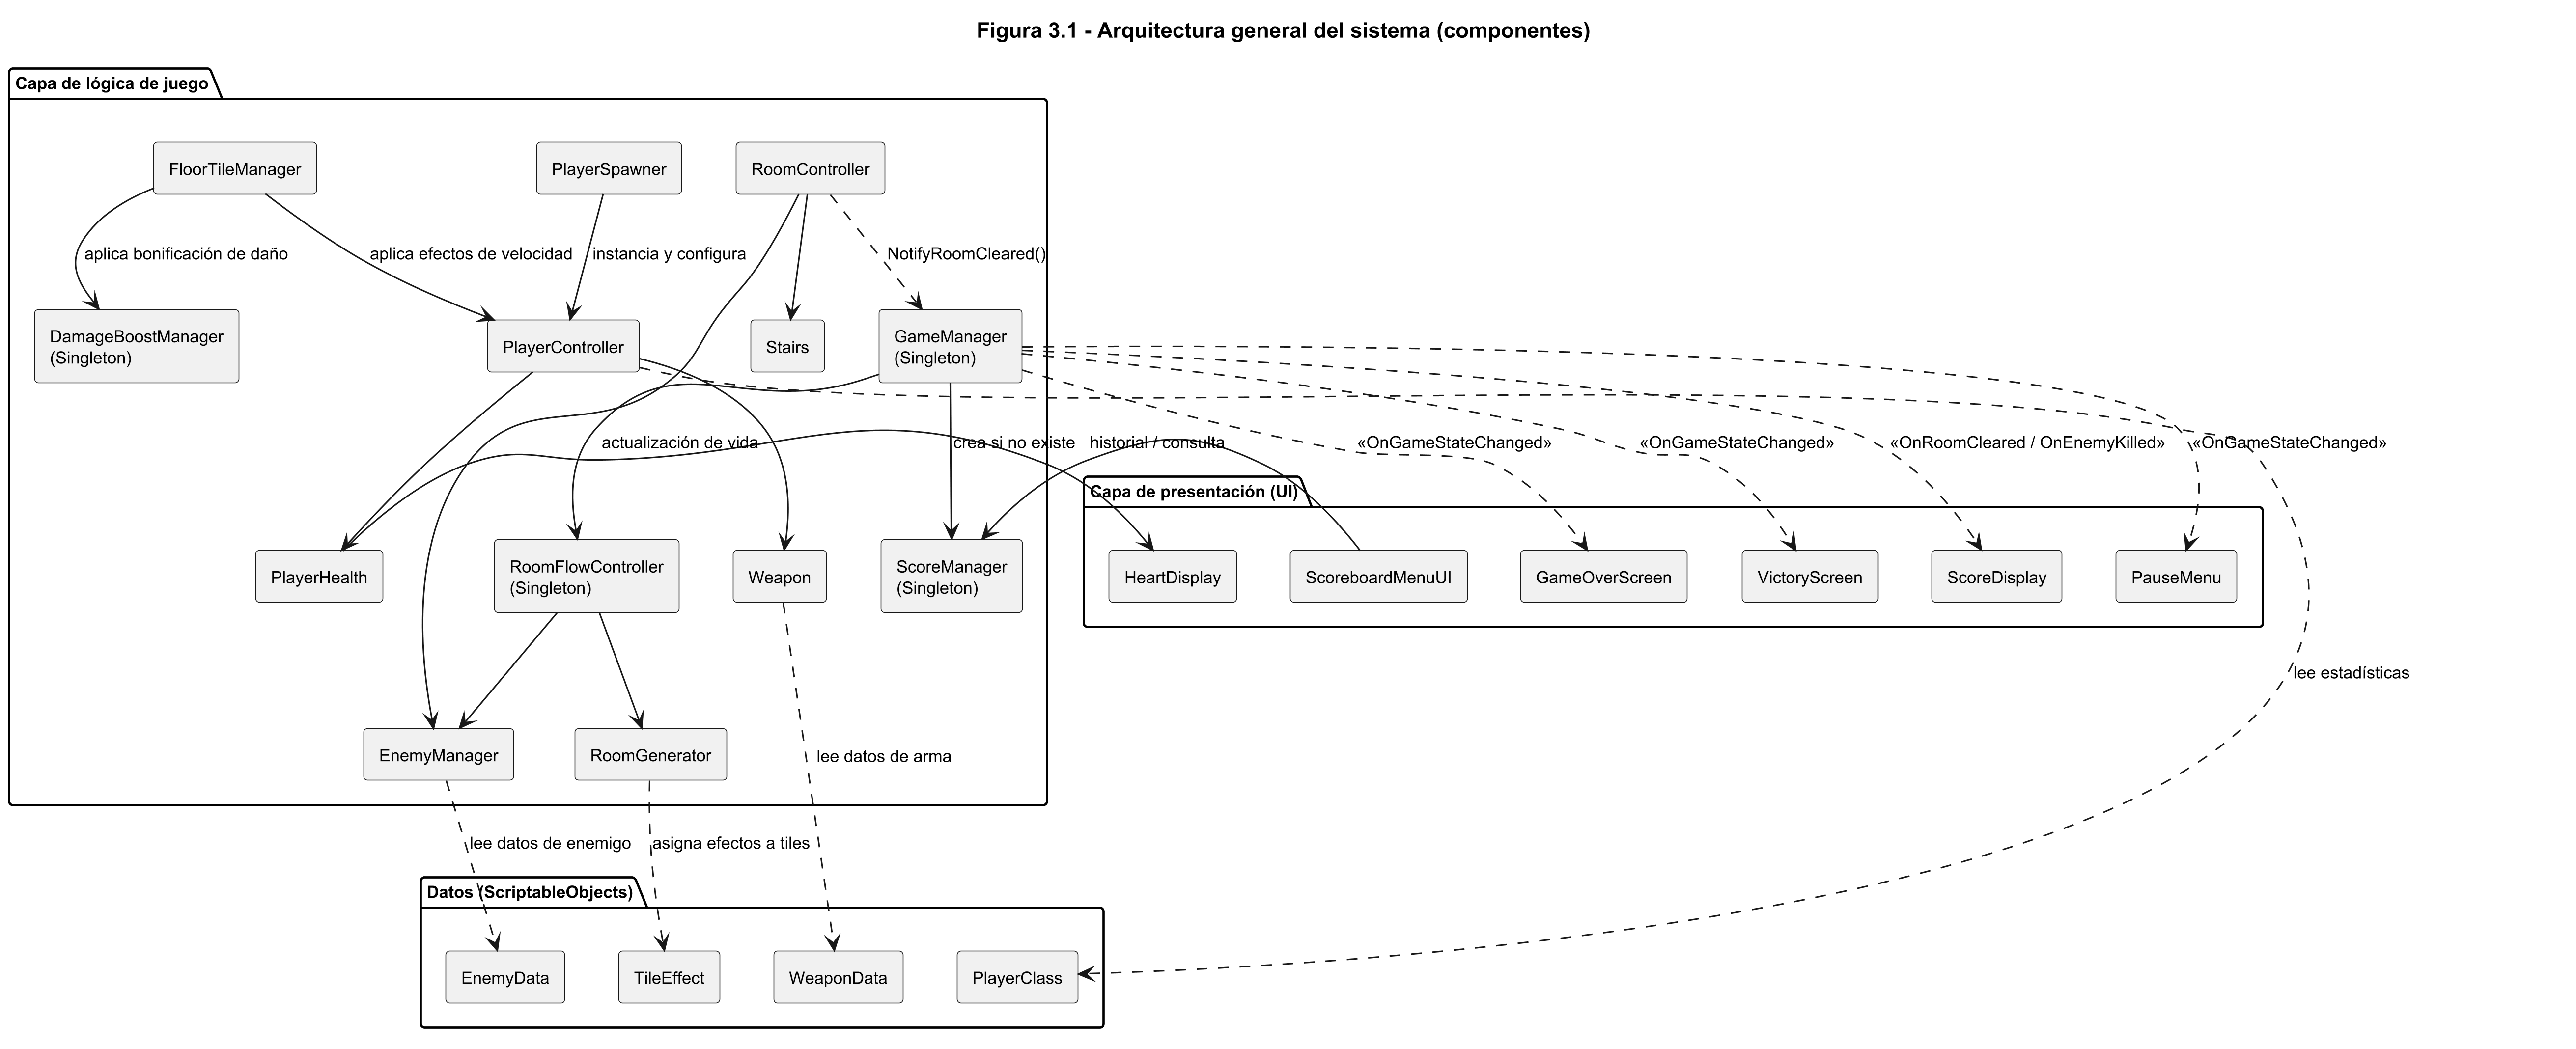
\includegraphics[width=0.95\textwidth]{Figuras/figura3_1_arquitectura_componentes.png}
\caption{
Diagrama de componentes de la arquitectura general del sistema. \textit{Elaboración propia.}
}
\label{fig:placeholder-1}
\end{center}
\end{figure}


\subsection{Flujo de escenas}


El proyecto se estructura en tres escenas de Unity que representan las fases del flujo de juego:

\begin{enumerate}
\item \textbf{MainMenu.} Escena del menú principal, con opciones para iniciar partida, consultar el historial de puntuaciones y salir del juego.
\item \textbf{ClassSelection.} Escena de selección de clase de personaje, donde el jugador elige entre las clases disponibles antes de comenzar la partida.
\item \textbf{GameScene.} Escena principal del juego, donde se desarrolla toda la acción. La generación procedural de salas se realiza dentro de esta misma escena, regenerando el contenido del \textit{tilemap} sin necesidad de cargar escenas adicionales.
\end{enumerate}

\begin{figure}[H]
\begin{center}
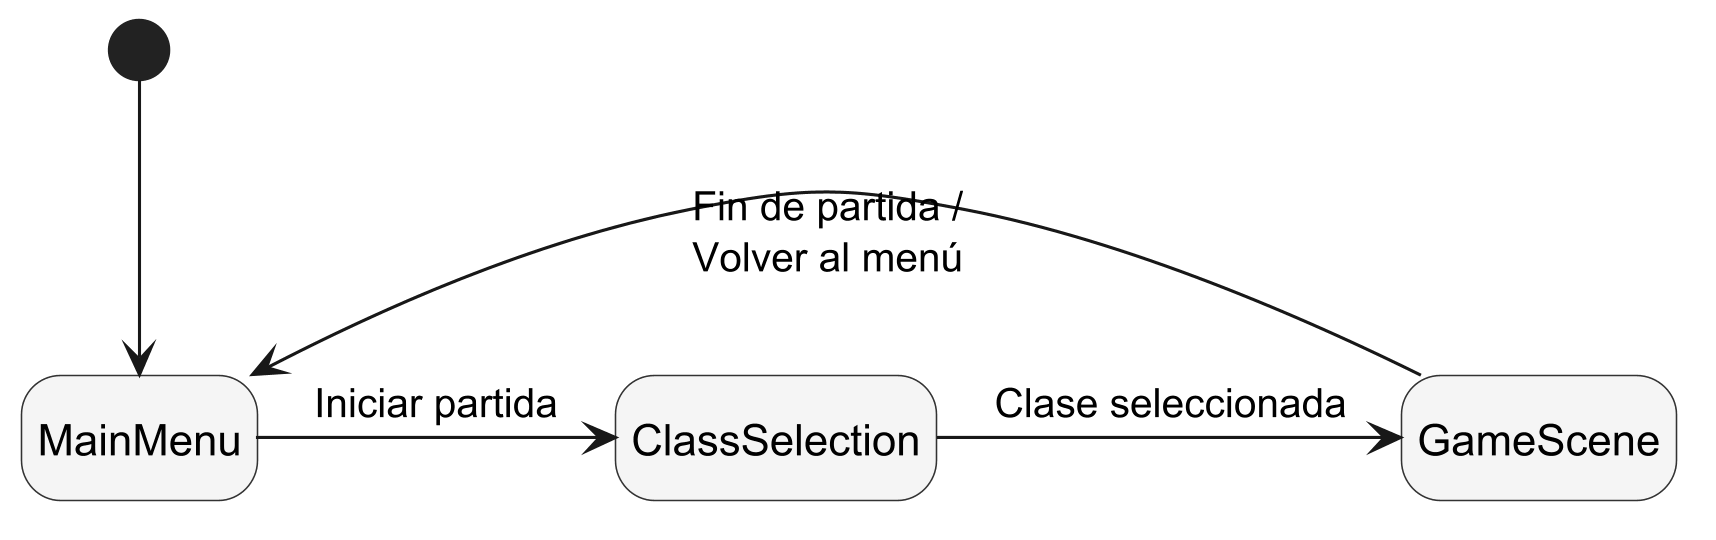
\includegraphics[width=0.95\textwidth]{Figuras/flujo_escenas_simple.png}
\caption{
Diagrama del flujo de escenas. \textit{Elaboración propia.}
}
\label{fig:placeholder-2}
\end{center}
\end{figure}


\subsection{Gestores centrales (\textit{managers})}


El sistema utiliza cuatro gestores centrales que implementan el patrón \textit{Singleton}. Tres de ellos (\texttt{GameManager}, \texttt{ScoreManager} y \texttt{DamageBoostManager}) persisten entre cambios de escena mediante \texttt{DontDestroyOnLoad} (directiva que evita que Unity destruya el objeto al cargar otra escena); el \texttt{RoomFlowController} opera como \textit{Singleton} de escena, re-instanciándose en cada escena de juego y re-enlazándose a los componentes necesarios mediante el evento \texttt{SceneManager.sceneLoaded}:

\begin{table}[H]
\begin{center}
\small
\begin{tabular}{|p{0.46\textwidth}|p{0.46\textwidth}|}
\hline
Gestor & Responsabilidad \\ \hline
\texttt{GameManager} & Control de estados del juego, progresión, transiciones entre escenas \\ \hline
\texttt{ScoreManager} & Cálculo de puntuación, persistencia del historial de partidas \\ \hline
\texttt{RoomFlowController} & Control del bucle de generación y progresión de salas \\ \hline
\texttt{DamageBoostManager} & Gestión de bonificaciones temporales de daño \\ \hline
\end{tabular}
\end{center}
\end{table}


\TablaTitulo{Gestores centrales del sistema.}

\subsection{Diagrama de dependencias}


La estructura de dependencias entre los módulos principales del sistema se organiza de la siguiente forma. El diagrama muestra la relación jerárquica entre componentes: cada nodo depende de los nodos situados debajo de él en la jerarquía. Las flechas indican dependencias de creación, referencia directa o suscripción a eventos. Los nodos marcados con \textit{(ScriptableObject)} representan activos de datos configurables desde el inspector de Unity.

\begin{figure}[H]
\begin{center}
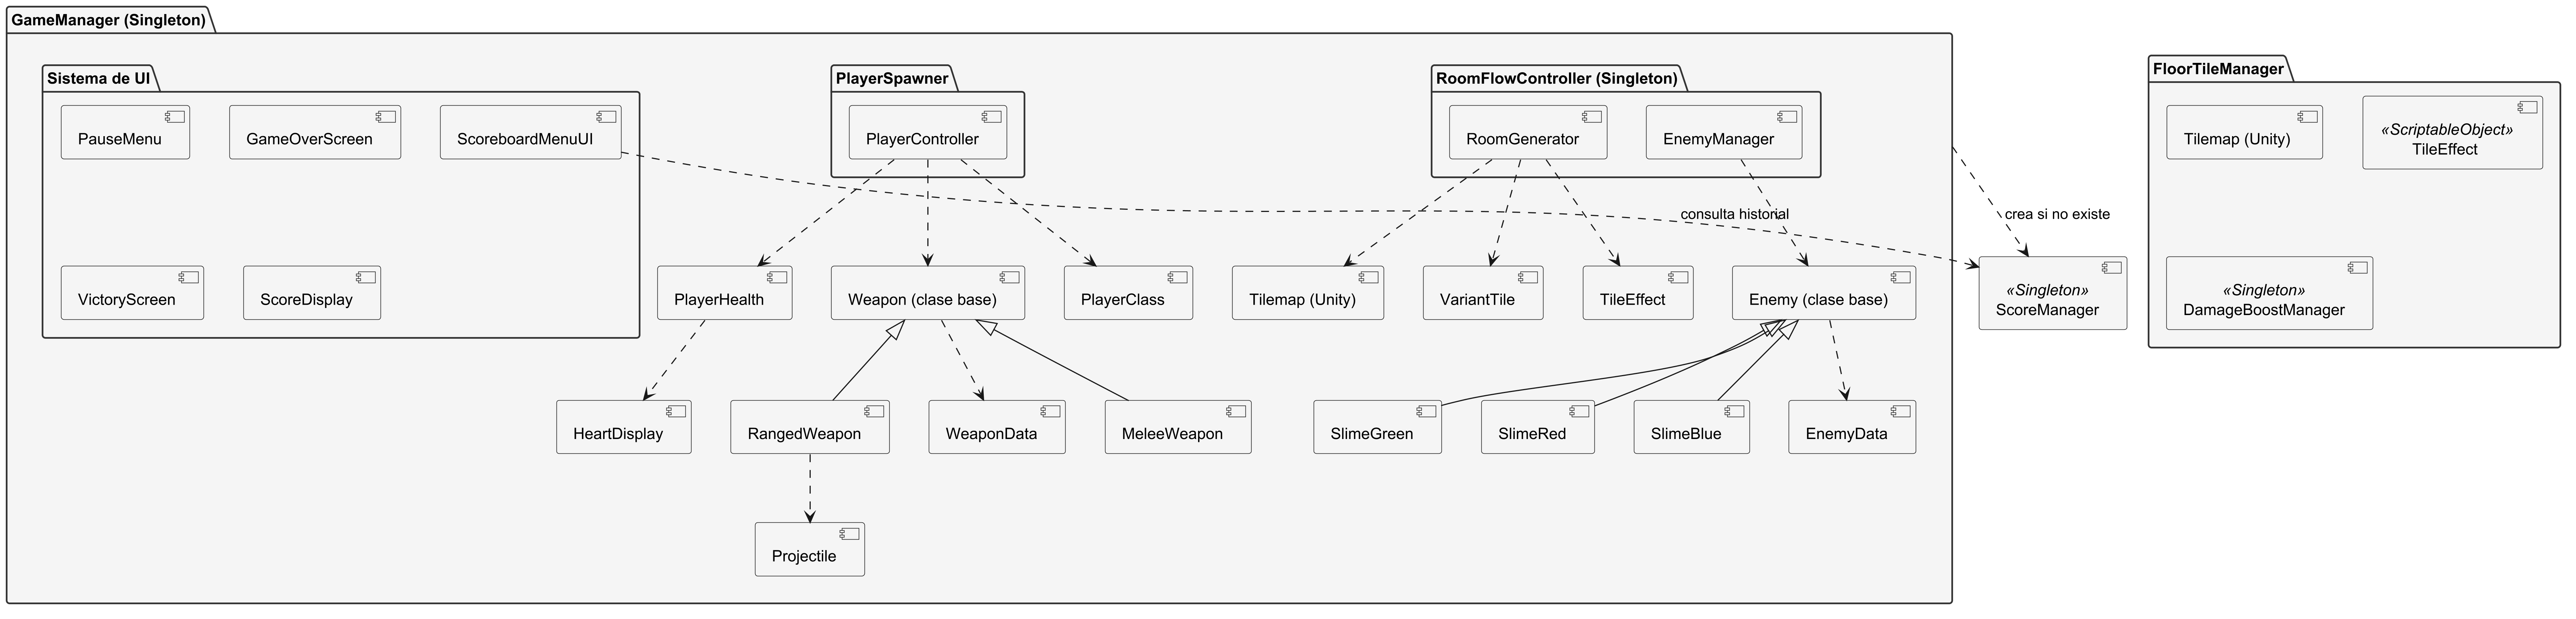
\includegraphics[width=0.95\textwidth]{Figuras/dependencias_modulos.png}
\caption{
Diagrama de dependencias entre los módulos del sistema. \textit{Elaboración propia.}
}
\label{fig:placeholder-4}
\end{center}
\end{figure}


\subsection{Flujo de producción: del activo gráfico al juego}


Esta sección describe el proceso completo de producción seguido para transformar los activos gráficos (\textit{sprites}) en entidades funcionales dentro del juego. El flujo abarca desde la creación e importación de los \textit{sprites} hasta la configuración de los \textit{GameObjects} con sus componentes de física, colisión y animación, y su posterior ensamblaje en la escena del juego.

\subsubsection{Importación y configuración de \textit{sprites}}


Los activos gráficos del proyecto se crearon en LibreSprite como \textit{pixel art} a resoluciones de 16x16, 32x32 y 64x64 píxeles, según el tipo de elemento (tiles, personajes y enemigos, respectivamente). Tras la exportación en formato PNG, la importación en Unity requiere una configuración específica para preservar la estética del \textit{pixel art}:

\begin{itemize}
\item \textbf{Pixels Per Unit (PPU):} se establece en 16 para que cada tile de 16x16 píxeles ocupe exactamente una unidad del mundo del juego. Esta correspondencia simplifica el cálculo de posiciones en el \textit{tilemap} y garantiza la coherencia entre la cuadrícula de tiles y las coordenadas del sistema de física.
\item \textbf{Filtrado:} se configura como \textit{Point (no filter)} para evitar el suavizado de bordes entre píxeles, preservando la apariencia nítida del \textit{pixel art}.
\item \textbf{Compresión:} se desactiva o se establece en modo sin pérdida (\textit{None}) para evitar artefactos visuales que distorsionarían los bordes de los \textit{sprites}.
\item \textbf{Modo de \textit{sprite}:} para personajes y enemigos con múltiples fotogramas de animación, se utiliza el modo \textit{Multiple}, que permite particionar una hoja de \textit{sprites} (\textit{spritesheet}) en fotogramas individuales mediante el editor de \textit{sprites} de Unity.
\end{itemize}

\begin{figure}[H]
\begin{center}
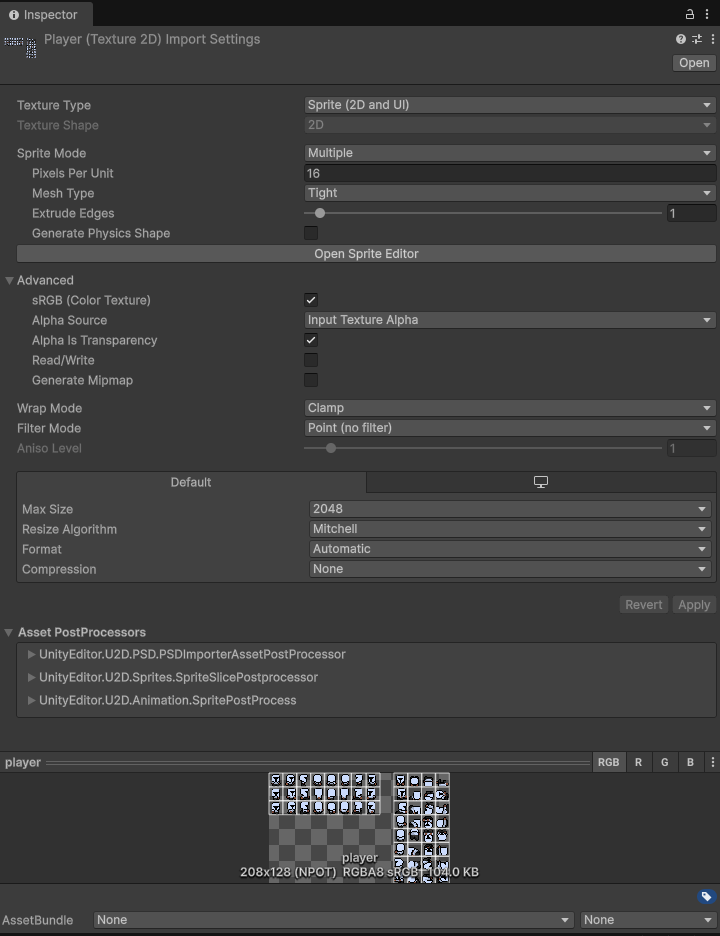
\includegraphics[width=0.9\textwidth]{Figuras/captura_9.png}
\caption{Configuración de importación de un \textit{sprite} en el inspector de Unity, mostrando los parámetros PPU, filtrado y compresión. \textit{Elaboración propia.}}
\label{fig:placeholder-6}
\end{center}
\end{figure}


\subsubsection{Creación de \textit{GameObjects} y configuración de componentes}


Cada entidad del juego se construye como un \textit{GameObject} de Unity al que se agregan los componentes necesarios para su funcionamiento. A continuación se describe la configuración típica para los principales tipos de entidad.

\textbf{Jugador:}
\begin{itemize}
\item \texttt{SpriteRenderer}: renderiza el \textit{sprite} del personaje con el orden de capa adecuado.
\item \texttt{Rigidbody2D}: habilita la simulación física con gravedad desactivada (movimiento cenital), detección de colisiones continua y rotación congelada.
\item \texttt{CircleCollider2D}: define el área física del personaje para la detección de colisiones con muros y enemigos. Se ha usado un colisionador circular en la zona central y desplazado hacia abajo para que las colisiones con muros sean más naturales (evitando que el jugador pueda quedar atrapado por colisionadores rectangulares en esquinas o bordes).
\item \texttt{PlayerController} (script): gestiona el movimiento y la esquiva.
\item \texttt{PlayerHealth} (script): gestiona los puntos de vida y la invulnerabilidad.
\item \texttt{Animator}: controla las transiciones entre estados de animación (reposo, movimiento, esquiva, daño).
\end{itemize}

\begin{figure}[H]
\begin{center}
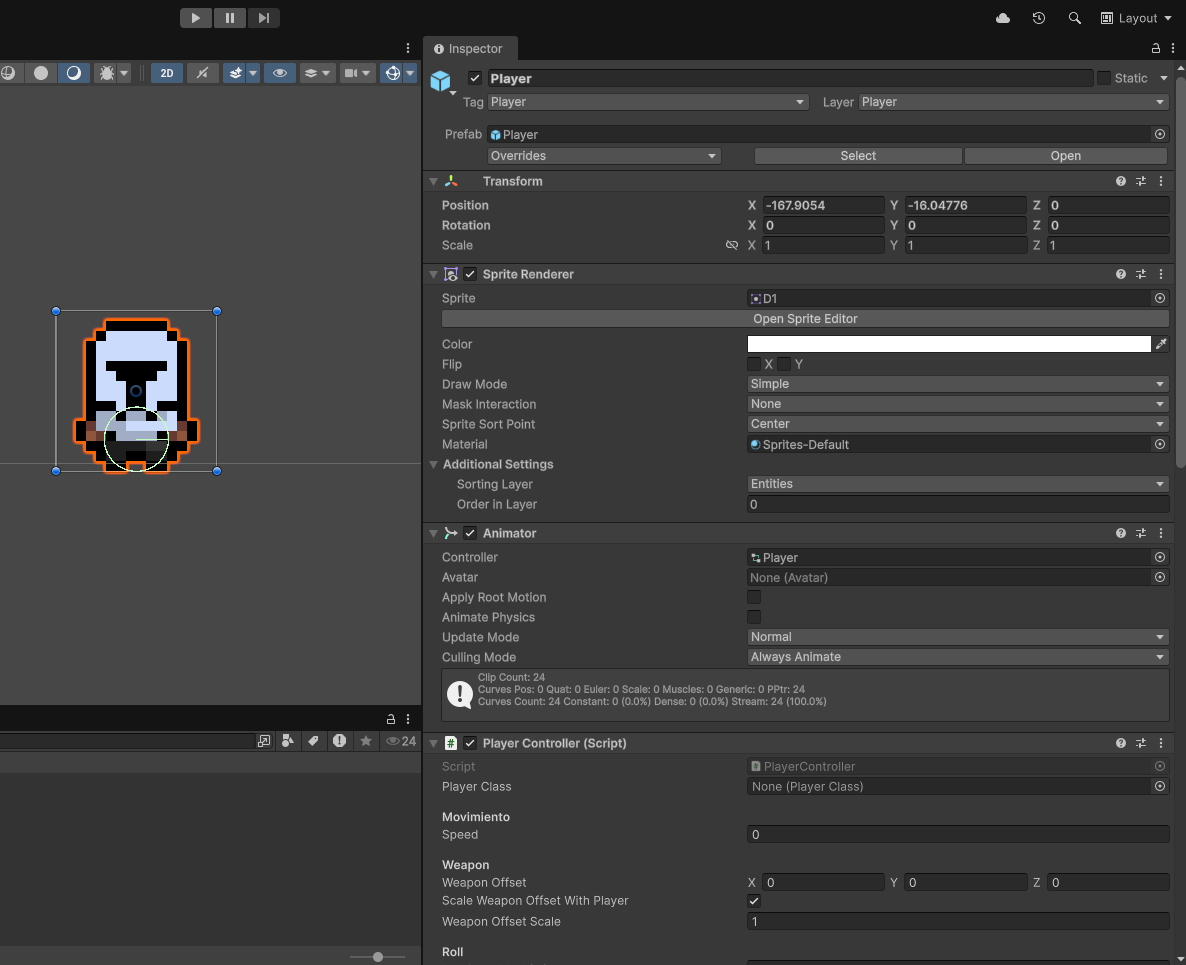
\includegraphics[width=0.9\textwidth]{Figuras/captura_10.png}
\caption{Vista del inspector de Unity mostrando los componentes configurados en el \textit{GameObject} del jugador: \textit{SpriteRenderer}, \textit{Rigidbody2D}, \textit{CircleCollider2D}, scripts y \textit{Animator}. \textit{Elaboración propia.}}
\label{fig:placeholder-7}
\end{center}
\end{figure}


\textbf{Enemigo (ejemplo: Slime Verde):}
\begin{itemize}
\item \texttt{SpriteRenderer}: renderiza el \textit{sprite} del enemigo.
\item \texttt{Rigidbody2D}: física 2D sin gravedad, con detección de colisiones continua.
\item \texttt{CircleCollider2D}: define el área de contacto del enemigo. Se utiliza un colisionador circular en lugar de rectangular porque la forma redondeada del \textit{slime} produce colisiones más naturales al contacto con el jugador y con los muros.
\item \texttt{SlimeGreen} (script): implementa la IA del enemigo francotirador.
\item \texttt{Animator}: gestiona las animaciones de movimiento, ataque y muerte.
\end{itemize}

\begin{figure}[H]
\begin{center}
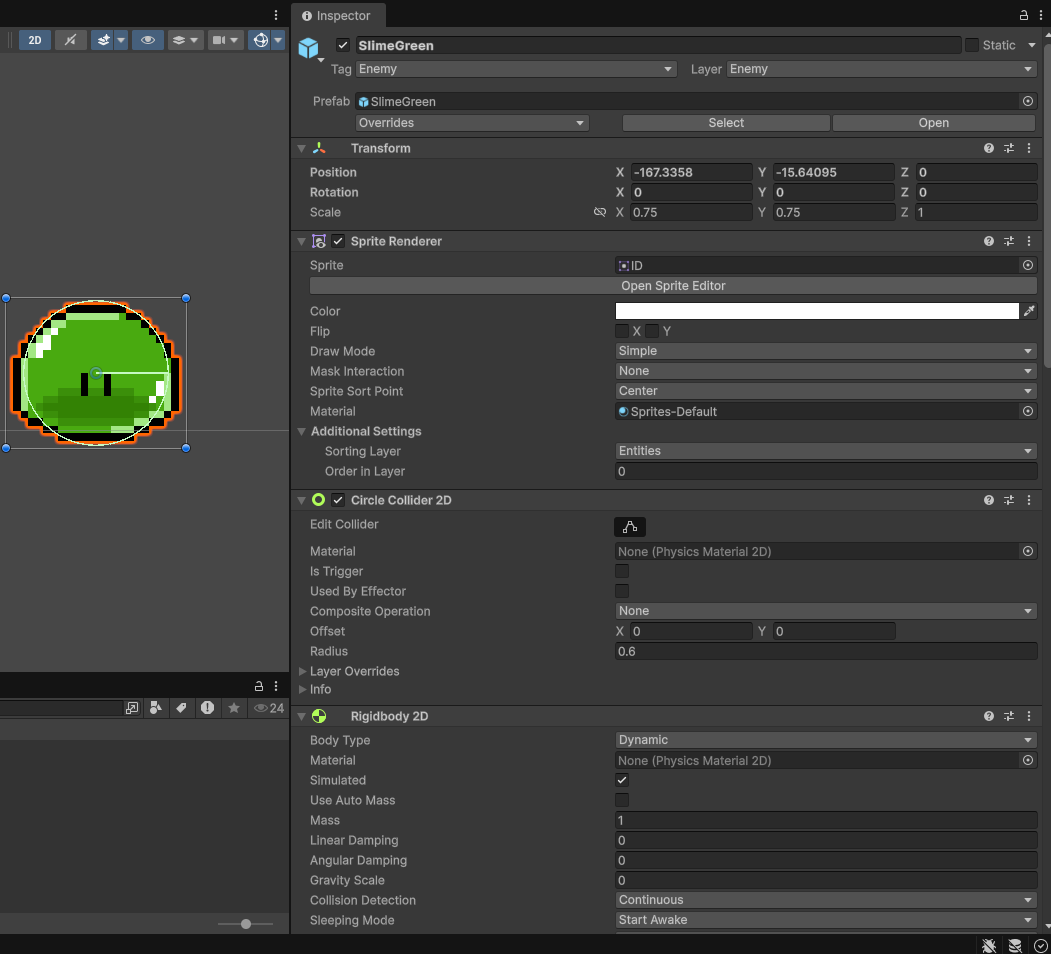
\includegraphics[width=0.9\textwidth]{Figuras/captura_11.png}
\caption{Vista del inspector de Unity mostrando los componentes de un enemigo \textit{Slime Verde}, con detalle del \textit{CircleCollider2D} y sus dimensiones. \textit{Elaboración propia.}}
\label{fig:placeholder-8}
\end{center}
\end{figure}


\subsubsection{Configuración de \textit{colliders} y \textit{hitboxes}}


La detección de colisiones se organiza en dos categorías:

\begin{itemize}
\item \textbf{\textit{Colliders} físicos} (modo no \textit{trigger}): producen respuesta física (empuje, bloqueo). Se utilizan en los muros perimetrales de las salas (\texttt{TilemapCollider2D} + \texttt{CompositeCollider2D} en el \textit{tilemap} de muros) y en el cuerpo del jugador y los enemigos, impidiendo que atraviesen paredes u otros objetos sólidos.
\item \textbf{\textit{Colliders de tipo trigger}} (modo \textit{Is Trigger} activado): detectan superposición sin respuesta física. Se utilizan para la detección de impactos de armas cuerpo a cuerpo (el \textit{hitbox} del arma), la detección de proyectiles contra enemigos o muros, la activación de escaleras al presionar la tecla de interacción y la detección de tiles especiales bajo el jugador o los enemigos.
\end{itemize}

La configuración del \textit{TilemapCollider2D} resulta especialmente relevante para la generación procedural. Al añadir un componente \texttt{TilemapCollider2D} al \textit{tilemap} de muros, Unity genera automáticamente un colisionador por cada tile presente en ese \textit{tilemap}. Combinado con un \texttt{CompositeCollider2D}, los colisionadores individuales se fusionan en un único colisionador perimetral continuo, lo que reduce el coste computacional de la simulación física y evita que el jugador pueda deslizarse entre los bordes de tiles adyacentes.

\subsubsection{Configuración de \textit{tilemaps} y tiles}


El sistema de niveles se construye sobre dos \textit{tilemaps} de Unity superpuestos en la misma escena:

\begin{enumerate}
\item \textbf{Tilemap de muros} (\texttt{wallTilemap}): contiene los tiles de muro que forman el perímetro de cada sala. Incluye los componentes \texttt{TilemapCollider2D} y \texttt{CompositeCollider2D} para generar la barrera física.
\item \textbf{Tilemap de suelo} (\texttt{floorTilemap}): contiene los tiles de suelo (normales y especiales) que componen el área jugable. No genera colisionadores, ya que el suelo no bloquea el movimiento.
\end{enumerate}

Cada tile se configura como un activo de tipo \texttt{VariantTile} (clase derivada de \texttt{TileBase} de Unity) que almacena múltiples variantes visuales del mismo tipo de tile. Al colocar un tile, el sistema selecciona una variante de forma determinista según la posición, lo que produce variabilidad visual sin aleatorización explícita.

\begin{figure}[H]
\begin{center}
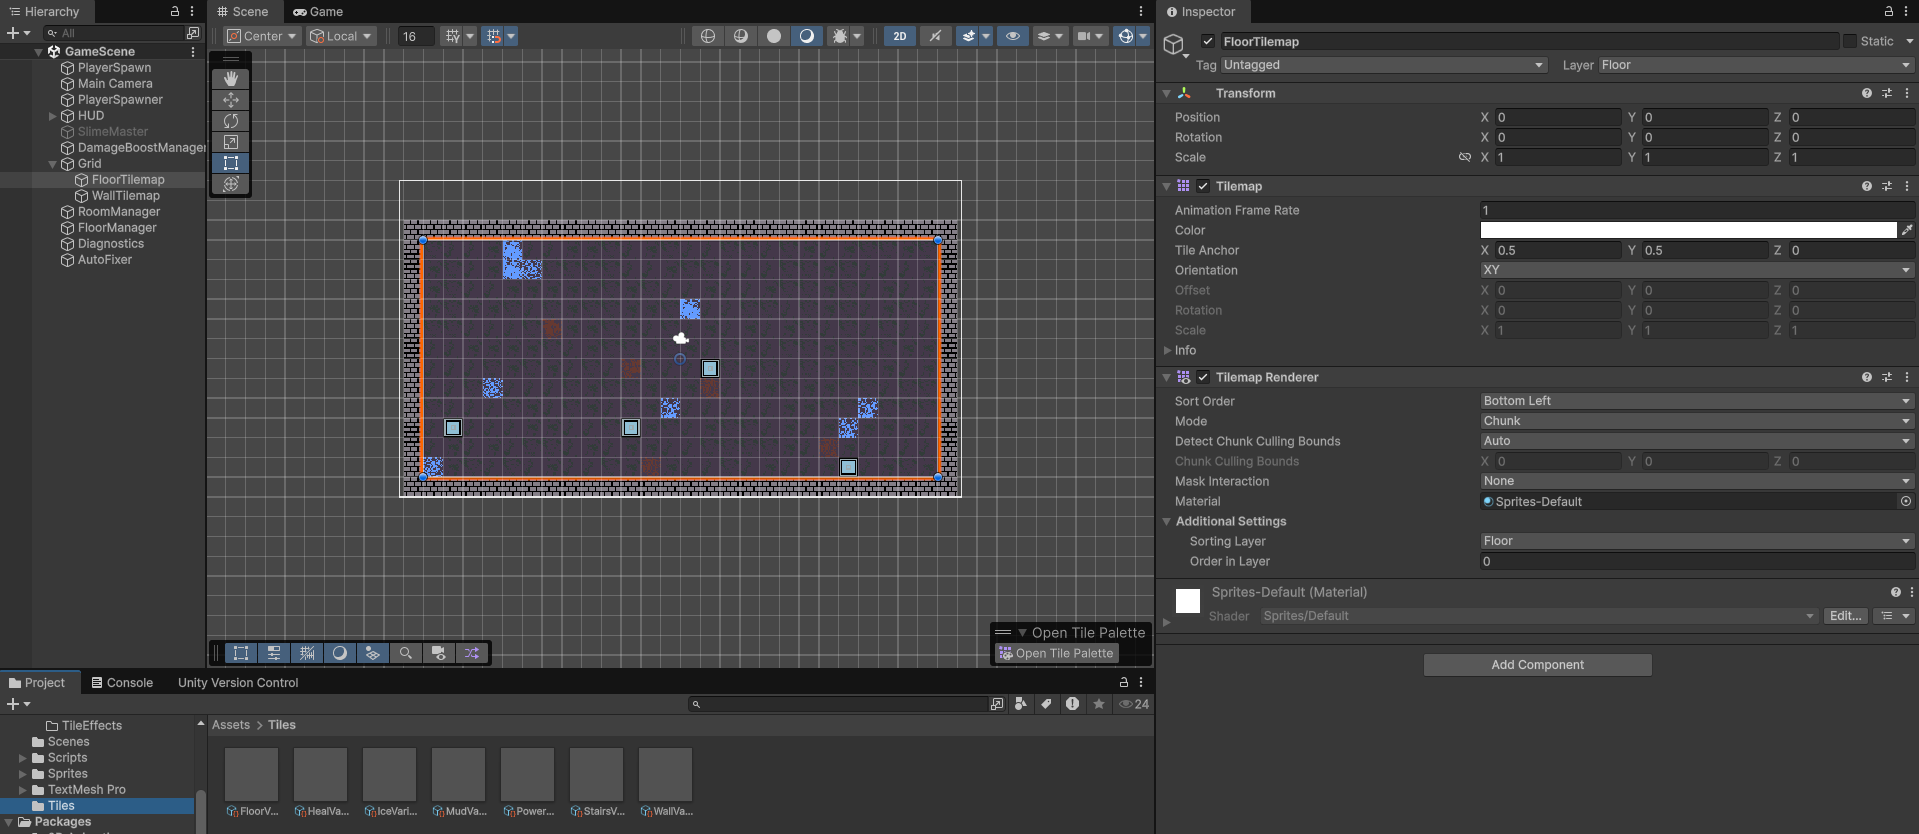
\includegraphics[width=0.9\textwidth]{Figuras/captura_12.png}
\caption{Editor de \textit{tilemaps} de Unity mostrando las dos capas (muros y suelo). \textit{Elaboración propia.}}
\label{fig:placeholder-10}
\end{center}
\end{figure}


\subsubsection{Sistema de animaciones}


Las animaciones del juego se implementan mediante el sistema de animación de Unity (\texttt{Animator} + \texttt{AnimationClip}). Cada personaje y enemigo dispone de un controlador de animación (\texttt{Animator Controller}) que define los estados de animación posibles y las transiciones entre ellos.

Para el jugador, los estados de animación incluyen:
\begin{itemize}
\item \textbf{Reposo} (\textit{idle}): animación cíclica de dos fotogramas con cadencia lenta.
\item \textbf{Movimiento} (\textit{walk}): animación cíclica de cuatro fotogramas. La dirección del movimiento (arriba, abajo, izquierda, derecha) se controla mediante parámetros del \textit{Animator} (\texttt{moveX}, \texttt{moveY}), lo que permite seleccionar la animación correspondiente a la dirección actual sin necesidad de un \textit{blend tree} completo.
\item \textbf{Esquiva} (\textit{roll}): animación de tres fotogramas que se reproduce una vez durante la duración de la esquiva.
\end{itemize}

Para los enemigos, los estados de animación incluyen reposo, movimiento y muerte, con transiciones controladas por parámetros del \textit{Animator} que los scripts de IA actualizan en cada fotograma.

\begin{figure}[H]
\begin{center}
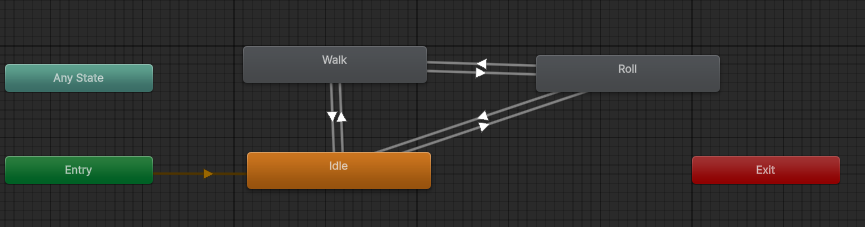
\includegraphics[width=0.9\textwidth]{Figuras/captura_13.png}
\caption{Controlador de animación (\textit{Animator Controller}) del jugador en Unity, mostrando los estados y las transiciones entre animaciones de reposo, movimiento y esquiva. \textit{Elaboración propia.}}
\label{fig:placeholder-11}
\end{center}
\end{figure}


\subsubsection{De los componentes al flujo de juego}


Una vez configurados los \textit{GameObjects} individuales con sus componentes, el flujo de juego se construye mediante la coordinación de estos elementos:

\begin{enumerate}
\item El \texttt{PlayerSpawner} instancia el \textit{prefab} del jugador en la posición inicial de la sala.
\item El \texttt{RoomGenerator} genera la estructura de tiles de la sala sobre los dos \textit{tilemaps} (muros y suelo).
\item El \texttt{EnemyManager} instancia los \textit{prefabs} de los enemigos en posiciones seguras dentro de la sala.
\item El \texttt{RoomFlowController} coordina la secuencia: bloqueo de escaleras -> combate -> habilitación de escaleras -> interacción -> siguiente sala.
\item El \texttt{GameManager} supervisa el estado global y gestiona las transiciones entre menú, juego, pausa, victoria y derrota.
\end{enumerate}

Cada \textit{prefab} contiene la configuración completa de su \textit{GameObject} (componentes, valores de campos serializados, referencias a \textit{ScriptableObjects}), de modo que al instanciarlo se obtiene una copia funcional del elemento sin necesidad de configuración adicional en tiempo de ejecución.


\section{Patrones y mecanismos de diseño aplicados}


En el apartado de estado del arte se presentaron los patrones de diseño seleccionados para el proyecto y la fundamentación teórica de cada uno. En este apartado se describe su aplicación concreta en la arquitectura de \textit{Ascension}: para cada patrón se presenta el código resultante y se analizan los detalles de implementación específicos del proyecto.

\subsection{Patrón \textit{Singleton}}


Como se fundamentó en el apartado correspondiente del estado del arte, el patrón \textit{Singleton} se seleccionó para los cuatro gestores centrales frente a la inyección de dependencias. Los tres gestores persistentes (\texttt{GameManager}, \texttt{ScoreManager}, \texttt{DamageBoostManager}) comparten la siguiente estructura:

\begin{lstlisting}
public static GameManager Instance { get; private set; }

void Awake() {
    if (Instance == null) {
        Instance = this;
        DontDestroyOnLoad(gameObject);
    } else {
        Destroy(gameObject);
    }
}
\end{lstlisting}


El \texttt{RoomFlowController} aplica la misma estructura de instancia única, pero omite \texttt{DontDestroy-}\texttt{OnLoad} porque sus referencias a componentes de escena (\texttt{RoomGenerator}, \texttt{EnemyManager}, \texttt{Tilemap}) se invalidan al cambiar de escena; en su lugar, se re-instancia en cada escena de juego y reconstruye sus referencias en el evento \texttt{SceneManager.sceneLoaded}.

\subsection{Patrón \textit{Observer}}


Como se describió en el análisis de patrones del estado del arte, el patrón \textit{Observer} desacopla el \texttt{GameManager} de los componentes de interfaz. Su implementación concreta utiliza los eventos \texttt{OnGameStateChanged}, \texttt{OnRoomCleared} y \texttt{OnEnemyKilled}:

\begin{lstlisting}
// En GameManager (emisor)
public delegate void GameStateChanged(GameState newState);
public static event GameStateChanged OnGameStateChanged;

// En PauseMenu (receptor)
void Start() {
    EnsureRuntimeUIIfMissing();
    WireButtonsOnce();
    GameManager.OnGameStateChanged += OnGameStateChanged;
}

private void OnGameStateChanged(GameState newState) {
    EnsureRuntimeUIIfMissing();
    if (pauseMenuPanel == null) return;
    pauseMenuPanel.SetActive(newState == GameState.Paused);
}
\end{lstlisting}


El \texttt{GameManager} desconoce cuántos ni cuáles componentes están suscritos, lo que permite añadir nuevos componentes reactivos (por ejemplo, un sistema de audio que reproduzca un efecto al completar una sala) sin modificar el código del gestor.

\subsection{Patrón \textit{Strategy}}


Como se describió en el análisis de patrones, el patrón \textit{Strategy} estructura el sistema de armas mediante subclases especializadas de \texttt{Weapon}. Cada tipo requiere campos específicos distintos (\texttt{swingAngle} para melee, \texttt{bulletPrefab} para ranged), lo que confirma la decisión de evitar condicionales internos:

\begin{lstlisting}
// Weapon es una clase concreta con Attack() virtual (cuerpo vacio);
// las subclases lo sobrescriben con su propio comportamiento.
public class Weapon : MonoBehaviour {
    public virtual void Attack() { }   // no-op de forma predeterminada
}

public class MeleeWeapon : Weapon {
    public override void Attack() {
        // Ataque de barrido con hitbox
    }
}

public class RangedWeapon : Weapon {
    public override void Attack() {
        // Disparo de proyectil
    }
}
\end{lstlisting}


El \texttt{PlayerController} interactúa con cualquier arma a través de la interfaz común \texttt{Weapon.Attack()}, sin necesidad de conocer el tipo concreto. Añadir un nuevo tipo de arma solo requiere crear una nueva subclase sin modificar el código existente.

\subsection{Patrón \textit{Template Method}}


Como se describió en el análisis de patrones, el patrón \textit{Template Method} estructura la jerarquía de enemigos. Sin este patrón, las alternativas serían: (a) tres clases independientes duplicando $\sim$180 líneas de lógica común, o (b) una única clase de $\sim$800 líneas con condicionales \texttt{switch(enemyType)}:

\begin{lstlisting}
public class Enemy : MonoBehaviour {
    protected virtual void Start() {
        // Inicializacion base: vida, fisica, gracia
    }
    
    protected virtual void Update() {
        // Logica base: verificacion de gracia, efectos de tiles
    }
    
    protected virtual void Die() {
        // Muerte base: notificacion, animacion, destruccion
    }
}

public class SlimeGreen : Enemy {
    protected override void Update() {
        base.Update();
        // Logica especifica: evaluar distancia, disparar
    }
}
\end{lstlisting}


La clase base \texttt{Enemy} define el esqueleto de comportamiento común (gestión de vida, detección de contacto, muerte, interacción con tiles), mientras que cada subclase especializa únicamente la inteligencia artificial, permitiendo añadir nuevos tipos de enemigo sin modificar las clases existentes.

\subsection{Arquitectura basada en componentes (Entidad-Componente)}


Además de los patrones clásicos, el análisis del estado del arte introdujo la arquitectura de componentes de Unity. Su aplicación en \textit{Ascension} responde al siguiente problema:

\textbf{Problema.} Las entidades del juego (jugador, enemigos, proyectiles) requieren combinaciones variables de funcionalidades: un enemigo necesita física, renderizado y lógica de IA, pero no control de entrada; el jugador necesita control de entrada, física, vida y arma, pero no lógica de IA.

\textbf{Alternativa descartada.} Herencia múltiple de una jerarquía profunda (\texttt{Entity > MovableEntity > DamageableEntity > PlayerEntity}). Se descartó porque C\# no soporta herencia múltiple y porque las jerarquías profundas producen clases base sobrecargadas con funcionalidad que no todas las subclases necesitan (el denominado \textit{fragile base class problem}).

\textbf{Aplicación en el proyecto:} Toda la arquitectura del juego se fundamenta en la composición de componentes proporcionada por Unity.

\begin{figure}[H]
\begin{center}
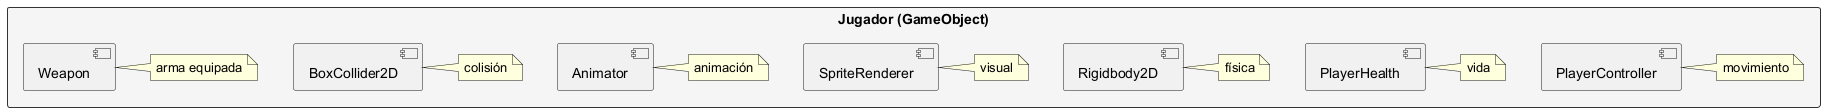
\includegraphics[width=0.95\textwidth]{Figuras/composicion_jugador.png}
\caption{
Diagrama de la composición del jugador. \textit{Elaboración propia.}
}
\label{fig:placeholder-14}
\end{center}
\end{figure}


\textbf{Justificación:} Favorece la composición sobre la herencia. Cada componente encapsula una responsabilidad única (movimiento, vida, física, renderizado), lo que permite reutilizar componentes entre entidades distintas y modificar una funcionalidad sin afectar a las demás. Por ejemplo, el componente \texttt{PlayerHealth} podría reutilizarse en un futuro NPC aliado sin necesidad de heredar de \texttt{PlayerController}.

\subsection{Máquina de estados (\textit{State Machine})}


Como se introdujo en el análisis del estado del arte, el \texttt{GameManager} implementa una máquina de estados. La decisión de diseño responde al siguiente problema:

\textbf{Problema.} El flujo global del juego atraviesa múltiples fases (menú, selección de clase, partida, pausa, fin de partida) con transiciones condicionadas. Sin una estructura explícita, el código del \texttt{GameManager} tendería a acumular variables booleanas (\texttt{isPaused}, \texttt{isGameOver}, \texttt{isInMenu}) cuyas combinaciones serían difíciles de mantener y probar.

\textbf{Alternativa descartada.} Variables booleanas independientes para cada estado. Se descartó porque $n$ booleanos producen $2^n$ combinaciones posibles, la mayoría de las cuales representan estados inválidos (por ejemplo, \texttt{isPaused == true} y \texttt{isGameOver == true} simultáneamente). Una enumeración con seis valores permite exactamente seis estados válidos, eliminando combinaciones ilógicas por construcción.

\textbf{Aplicación en el proyecto:} Control del flujo global del juego en \texttt{GameManager}.

\begin{figure}[H]
\begin{center}
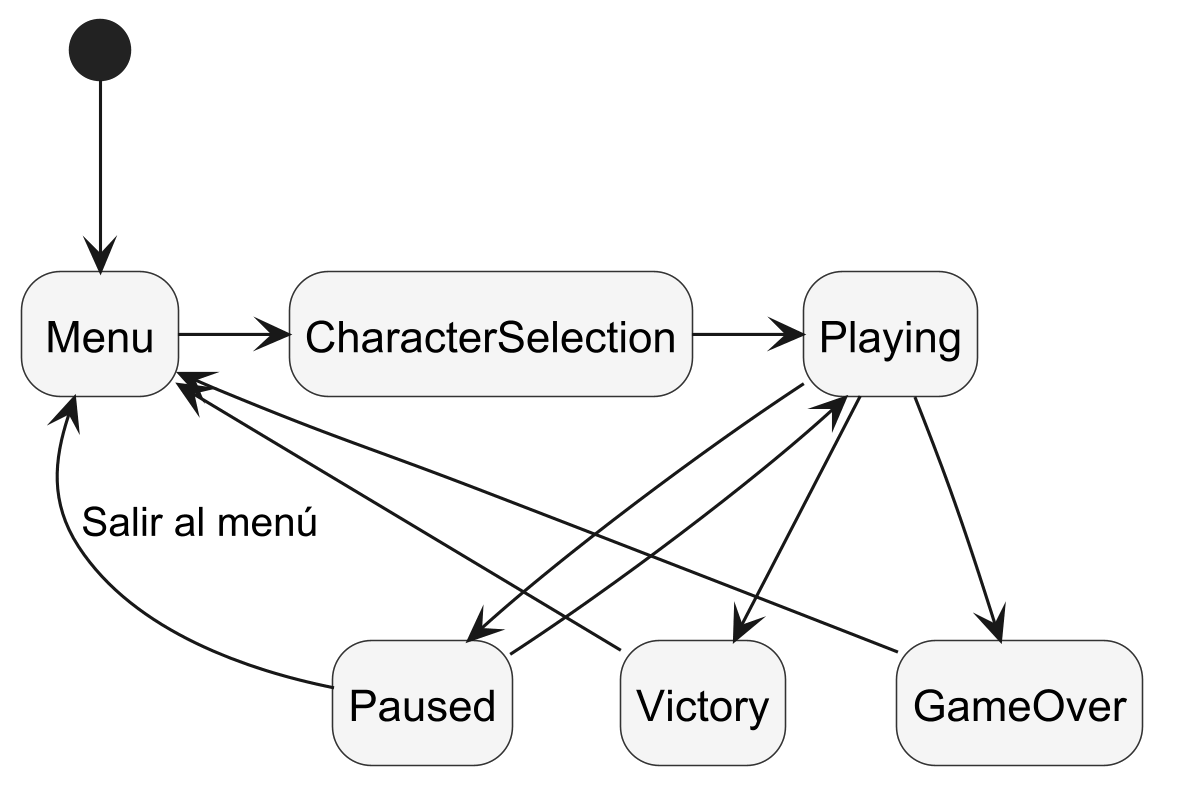
\includegraphics[width=0.95\textwidth]{Figuras/estados_juego.png}
\caption{
Diagrama de los estados del juego. \textit{Elaboración propia.}
}
\label{fig:placeholder-15}
\end{center}
\end{figure}


\textbf{Justificación:} Modela de forma explícita los estados válidos del juego y las transiciones permitidas entre ellos, reduciendo la probabilidad de estados no contemplados y facilitando la comprensión del flujo del juego.

\subsection{Interacción entre patrones: análisis de flujos transversales}


Los patrones descritos en las secciones anteriores no operan de forma aislada, sino que se combinan en cadenas de interacción que atraviesan múltiples subsistemas. A continuación se analizan tres flujos representativos que ilustran cómo la combinación de patrones produce un diseño cohesivo con bajo acoplamiento.

\subsubsection{Flujo 1: Muerte de un enemigo (\textit{Template Method} + \textit{Observer} + \textit{Singleton})}


Cuando un enemigo es eliminado, intervienen tres patrones en cadena. El patrón \textit{Template Method} proporciona el método \texttt{Die()} en la clase base \texttt{Enemy}, que todas las subclases heredan sin sobrescribir. Este método invoca al \texttt{GameManager} -- accesible globalmente mediante el patrón \textit{Singleton} -- a través del método \texttt{NotifyEnemyKilled()}. A su vez, el \texttt{GameManager} emite el evento \texttt{OnEnemyKilled} del patrón \textit{Observer}, al que están suscritos los componentes de interfaz de usuario.

\begin{lstlisting}
// (1) Template Method: Enemy.Die() -- heredado por SlimeGreen, SlimeRed, SlimeBlue
protected virtual void Die() {
    if (isDead) return;
    isDead = true;
    
    // (2) Singleton: acceso global al GameManager
    if (GameManager.Instance != null) {
        int scoreValue = enemyData != null ? enemyData.damage * 5 : 10;
        GameManager.Instance.NotifyEnemyKilled(scoreValue);
    }
    
    if (animator != null && animator.runtimeAnimatorController != null && hasAnimDieTrigger) {
        animator.SetTrigger("Die");
        Destroy(gameObject, 0.5f);
    } else {
        Destroy(gameObject);
    }
}

// (3) Observer: GameManager emite evento que la UI recibe
public void NotifyEnemyKilled(int scoreValue = 10) {
    enemiesKilled++;
    ScoreManager.Instance?.Add(scoreValue);     // Singleton: acceso al ScoreManager
    OnEnemyKilled?.Invoke(enemiesKilled);       // Observer: notifica a la UI
}
\end{lstlisting}


La cadena completa es: \textbf{Template Method} (el esqueleto de \texttt{Die()} se define una sola vez) -> \textbf{Singleton} (acceso al gestor central sin propagación de referencias) -> \textbf{Observer} (desacoplamiento entre la lógica de muerte y la interfaz de usuario). Si se hubiera implementado sin estos patrones, cada subclase de enemigo habría necesitado duplicar la lógica de muerte, mantener una referencia explícita al \texttt{GameManager} (pasada por constructor o asignada en el inspector) y conocer directamente los componentes de UI que deben actualizarse.

\subsubsection{Flujo 2: Ataque del jugador (\textit{Strategy} + \textit{ScriptableObject} + \textit{Singleton})}


Cuando el jugador ataca, intervienen el patrón \textit{Strategy}, el sistema de \textit{ScriptableObjects} y el patrón \textit{Singleton}. El \texttt{PlayerController} invoca \texttt{weapon.Attack()} a través de la interfaz común de la clase base \texttt{Weapon} (\textit{Strategy}), sin conocer si el arma es cuerpo a cuerpo o a distancia. La implementación concreta -- definida en \texttt{MeleeWeapon} o \texttt{RangedWeapon} -- consulta los parámetros del \textit{ScriptableObject} \texttt{WeaponData} para obtener el daño base y, en el caso de las armas a distancia, el prefab del proyectil. El proyectil, a su vez, consulta al \texttt{DamageBoostManager} (\textit{Singleton}) para aplicar las bonificaciones de daño de los tiles de potenciación.

\begin{lstlisting}
// (1) Strategy: el PlayerController no distingue entre tipos de arma
weapon.Attack();    // Polimorfismo: ejecuta MeleeWeapon.Attack() o RangedWeapon.Attack()

// (2) ScriptableObject: el arma consulta sus parametros de un activo externo
public override void Attack() {
    // ...
    projectileScript.damage = weaponData.damage;   // Dato del ScriptableObject
}

// (3) Singleton: el proyectil consulta al gestor de bonificacion
void Start() {
    damage = DamageBoostManager.Instance.GetBoostedDamage(damage);  // Singleton
}
\end{lstlisting}


\subsubsection{Flujo 3: Cambio de estado del juego (\textit{State Machine} + \textit{Observer} + \textit{Singleton})}


La transición de estado del juego ejemplifica la interacción entre la máquina de estados, el patrón \textit{Observer} y el patrón \textit{Singleton}. Cuando el jugador pulsa la tecla de pausa, el \texttt{PauseMenu} accede al \texttt{GameManager} mediante el \textit{Singleton} y solicita un cambio de estado. La máquina de estados del \texttt{GameManager} procesa la transición (modifica \texttt{Time.timeScale}, actualiza la variable \texttt{currentState}) y emite el evento \texttt{OnGameStateChanged} del patrón \textit{Observer}. Todos los componentes suscritos -- incluido el propio \texttt{PauseMenu} que originó la petición -- reaccionan al evento de forma independiente.

\begin{lstlisting}
// (1) Singleton: acceso al gestor central desde cualquier componente
GameManager.Instance.ChangeState(GameState.Paused);

// (2) State Machine: procesamiento de la transicion
public void ChangeState(GameState newState) {
    currentState = newState;
    Time.timeScale = newState == GameState.Playing ? 1f : 0f;
    
    // (3) Observer: notificacion a todos los suscriptores
    OnGameStateChanged?.Invoke(newState);
}

// (4) Suscriptores independientes reaccionan sin acoplamiento
// PauseMenu:
private void OnGameStateChanged(GameState state) {
    EnsureRuntimeUIIfMissing();
    if (pauseMenuPanel == null) return;
    pauseMenuPanel.SetActive(state == GameState.Paused);
}
// GameOverScreen:
private void OnGameStateChanged(GameState state) {
    gameOverPanel.SetActive(state == GameState.GameOver);
}
\end{lstlisting}


Esta interacción demuestra una propiedad arquitectónica: el emisor del evento (\texttt{GameManager}) no conoce ni la cantidad ni la identidad de los suscriptores, lo que permite añadir nuevos componentes reactivos -- por ejemplo, un futuro sistema de audio que silencie la música al pausar -- sin modificar el código del \texttt{GameManager} ni de los suscriptores existentes.

\chapter{Desarrollo de Ascension}


El presente capítulo constituye el núcleo técnico de la memoria y describe la implementación detallada de cada subsistema del videojuego \textit{Ascension}. Partiendo del diseño presentado previamente -- requisitos, arquitectura y patrones de diseño --, se documenta cada módulo con sus correspondientes fragmentos de código, explicaciones línea por línea y diagramas de interacción. Al final del capítulo se describen dos sistemas desarrollados pero pendientes de integración completa en el flujo de juego.

El desarrollo de cada subsistema siguió la metodología iterativa e incremental descrita en la introducción. Las secciones de este capítulo presentan el resultado final de cada módulo tras las iteraciones realizadas; al inicio de cada sección se incluye un breve párrafo de \textbf{evolución iterativa} que documenta los cambios de diseño más relevantes que se produjeron durante el proceso de desarrollo, proporcionando trazabilidad entre la metodología adoptada y las decisiones técnicas finales.

\section{Sistema de gestión central}


\textbf{Evolución iterativa.} El sistema de gestión central atravesó tres iteraciones significativas. En la primera versión, el \texttt{GameManager} gestionaba directamente la generación de salas, la aparición de enemigos y la puntuación en una única clase monolítica de más de 500 líneas. La validación funcional reveló que esta concentración de responsabilidades dificultaba la depuración -- un error en la generación de salas afectaba a la lógica de puntuación -- y violaba el principio de responsabilidad única. En la segunda iteración se extrajeron el \texttt{RoomFlowController}, el \texttt{ScoreManager} y el \texttt{DamageBoostManager} como gestores independientes, cada uno con su propio ciclo de vida \textit{Singleton}. La tercera iteración introdujo el sistema de eventos (\texttt{OnGameStateChanged}, \texttt{OnRoomCleared}, \texttt{OnEnemyKilled}) para desacoplar la comunicación entre gestores: en la versión anterior, el \texttt{GameManager} invocaba métodos concretos de cada componente de UI, lo que obligaba a modificar el gestor central cada vez que se añadía un nuevo elemento a la interfaz.

\subsection{GameManager: controlador principal del juego}


El \texttt{GameManager} constituye el componente central del sistema. Implementa el patrón \textit{Singleton} con el objetivo de mantener una única instancia, y gestiona el ciclo de vida completo de una partida mediante una máquina de estados finitos (FSM). Sus responsabilidades incluyen el control de estados del juego, la gestión de progresión (salas completadas, enemigos eliminados), las transiciones entre escenas y la coordinación de los subsistemas.

\textbf{Máquina de estados.} El flujo del juego se modela mediante una enumeración que define los estados válidos:

\begin{lstlisting}
public enum GameState {
    Menu,
    CharacterSelection,
    Playing,
    Paused,
    GameOver,
    Victory
}
\end{lstlisting}


Las transiciones entre estados se gestionan mediante un método centralizado que modifica el estado actual, ajusta la escala de tiempo del juego y notifica a los observadores suscritos:

\begin{lstlisting}
public void ChangeState(GameState newState) {
    if (currentState == newState) return;    // Evita transiciones redundantes
    
    currentState = newState;
    
    switch (newState) {
        case GameState.Playing:
            Time.timeScale = 1f;             // Tiempo normal: fisica y animaciones activas
            isPaused = false;
            break;
        case GameState.Paused:
            Time.timeScale = 0f;             // Detiene la simulacion completa
            isPaused = true;
            break;
        case GameState.GameOver:
        case GameState.Victory:
            Time.timeScale = 0f;             // Congela el juego tras el resultado
            break;
    }
    
    OnGameStateChanged?.Invoke(newState);    // Notifica a todos los suscriptores
}
\end{lstlisting}


Línea por línea:

\begin{itemize}
\item \texttt{if (currentState == newState) return}: previene notificaciones duplicadas si un componente solicita transitar al estado en el que ya se encuentra el juego, lo que evitaría efectos colaterales como reactivar paneles de UI que ya están visibles.
\item \texttt{Time.timeScale = 0f}: detiene toda la simulación dependiente del tiempo escalado (física del \texttt{Rigidbody2D}, animaciones del \texttt{Animator}, corutinas que usen \texttt{WaitForSeconds}). Se seleccionó \texttt{Time.timeScale} frente a la alternativa de desactivar componentes individuales porque proporciona una pausa global con una sola asignación, sin necesidad de iterar sobre todos los objetos activos de la escena.
\item \texttt{OnGameStateChanged?.Invoke(newState)}: emite el evento del patrón \textit{Observer}. El operador \texttt{?.} evita una excepción si ningún componente está suscrito al evento. Los componentes de UI (\texttt{PauseMenu}, \texttt{GameOverScreen}) se suscriben a este evento en su método \texttt{Start()} y reaccionan automáticamente al cambio de estado.
\end{itemize}

\begin{figure}[H]
\begin{center}
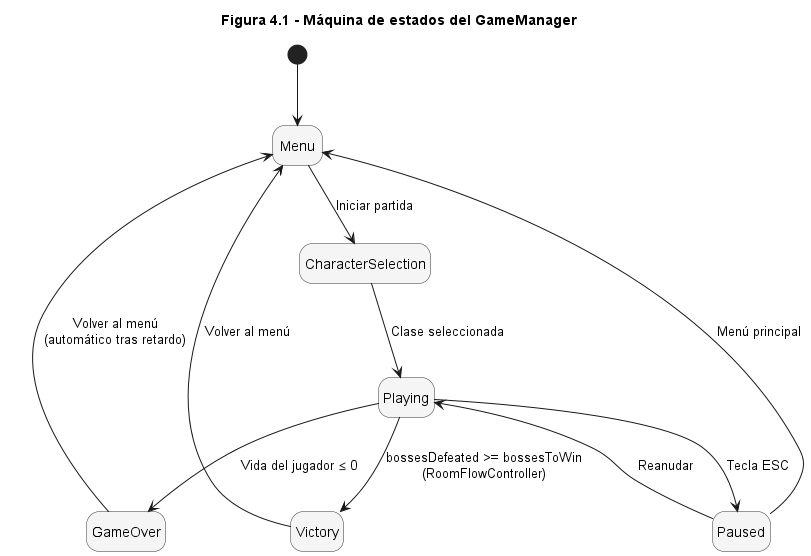
\includegraphics[width=0.95\textwidth,height=0.72\textheight,keepaspectratio]{Figuras/figura4_1_gamemanager_estados.png}
\caption{
Diagrama de estados UML del \texttt{GameManager}. \textit{Elaboración propia.}
}
\label{fig:placeholder-1}
\end{center}
\end{figure}


\textbf{Patrón Singleton.} La inicialización del \textit{Singleton} se realiza en el método \texttt{Awake()}, con el objetivo de que solo exista una instancia del gestor y que esta persista entre cambios de escena:

\begin{lstlisting}
void Awake() {
    if (Instance == null) {
        Instance = this;
        
        if (ScoreManager.Instance == null) {
            new GameObject("ScoreManager").AddComponent<ScoreManager>();
        }
        DontDestroyOnLoad(gameObject);
    } else {
        Destroy(gameObject);
        return;
    }
}
\end{lstlisting}


La comprobación \texttt{if (Instance == null)} previene la creación de instancias duplicadas cuando se vuelve a cargar una escena que contenga un \texttt{GameManager} en su jerarquía. Adicionalmente, si no existe un \texttt{ScoreManager} activo, el \texttt{GameManager} lo crea de forma automática, de forma que el sistema de puntuación esté disponible. La llamada a \texttt{DontDestroyOnLoad} se realiza al final del bloque para que tanto el \texttt{GameManager} como el \texttt{ScoreManager} recién creado persistan entre cambios de escena. Si ya existe una instancia, el duplicado se destruye y se retorna inmediatamente con \texttt{return}.

\textbf{Sistema de eventos.} El \texttt{GameManager} expone tres eventos principales que implementan el patrón \textit{Observer}:

\begin{table}[H]
\begin{center}
\small
\begin{tabular}{|p{0.307\textwidth}|p{0.307\textwidth}|p{0.307\textwidth}|}
\hline
\textbf{Evento} & \textbf{Momento de emisión} & \textbf{Suscriptores típicos} \\ \hline
\texttt{OnGameStateChanged} & Al cambiar el estado del juego & \texttt{PauseMenu}, pantallas de fin de partida, sistemas de UI \\ \hline
\texttt{OnRoomCleared} & Al completar una sala & \texttt{RoomFlowController}, \texttt{ScoreDisplay} \\ \hline
\texttt{OnEnemyKilled} & Al eliminar un enemigo & \texttt{ScoreManager}, contadores de UI \\ \hline
\end{tabular}
\end{center}
\end{table}


\TablaTitulo{Eventos del \texttt{GameManager}.
}

\textbf{Inicio de partida y coordinación entre gestores.} El método \texttt{StartNewRun()} constituye el punto de entrada de cada nueva partida y ejemplifica la coordinación entre los cuatro gestores \textit{Singleton} del sistema. Al iniciar una ejecución, el \texttt{GameManager} reinicia sus propios contadores y delega el reinicio de cada subsistema en el gestor correspondiente:

\begin{lstlisting}
public void StartNewRun() {
    currentLevel = 1;
    roomsCleared = 0;
    enemiesKilled = 0;
    
    RoomFlowController.Instance?.ResetRunProgress();   // Reinicia profundidad de sala y secuencia de jefes
    ScoreManager.Instance?.ResetScore();               // Pone la puntuacion a cero
    DamageBoostManager.Instance?.ResetBoost();          // Elimina bonificaciones de dano residuales
    
    ChangeState(GameState.Playing);                    // Transita a Playing -> Time.timeScale = 1
}
\end{lstlisting}


La secuencia de reinicio sigue un orden específico: primero se reinician los datos del \texttt{GameManager}, después los de cada gestor dependiente y, finalmente, se cambia el estado a \texttt{Playing}. Este orden garantiza que los subsistemas estén en un estado limpio \textit{antes} de que la transición de estado notifique a los suscriptores del evento \texttt{OnGameStateChanged} -- incluida la interfaz de usuario, que al recibir la notificación de estado \texttt{Playing} consulta los contadores, que ya deben estar a cero. Si el cambio de estado se realizase antes de los reinicios, los componentes de UI mostrarían brevemente los datos de la partida anterior.

El siguiente diagrama resume la cadena de coordinación entre gestores al iniciar una nueva partida:

\begin{figure}[H]
\begin{center}
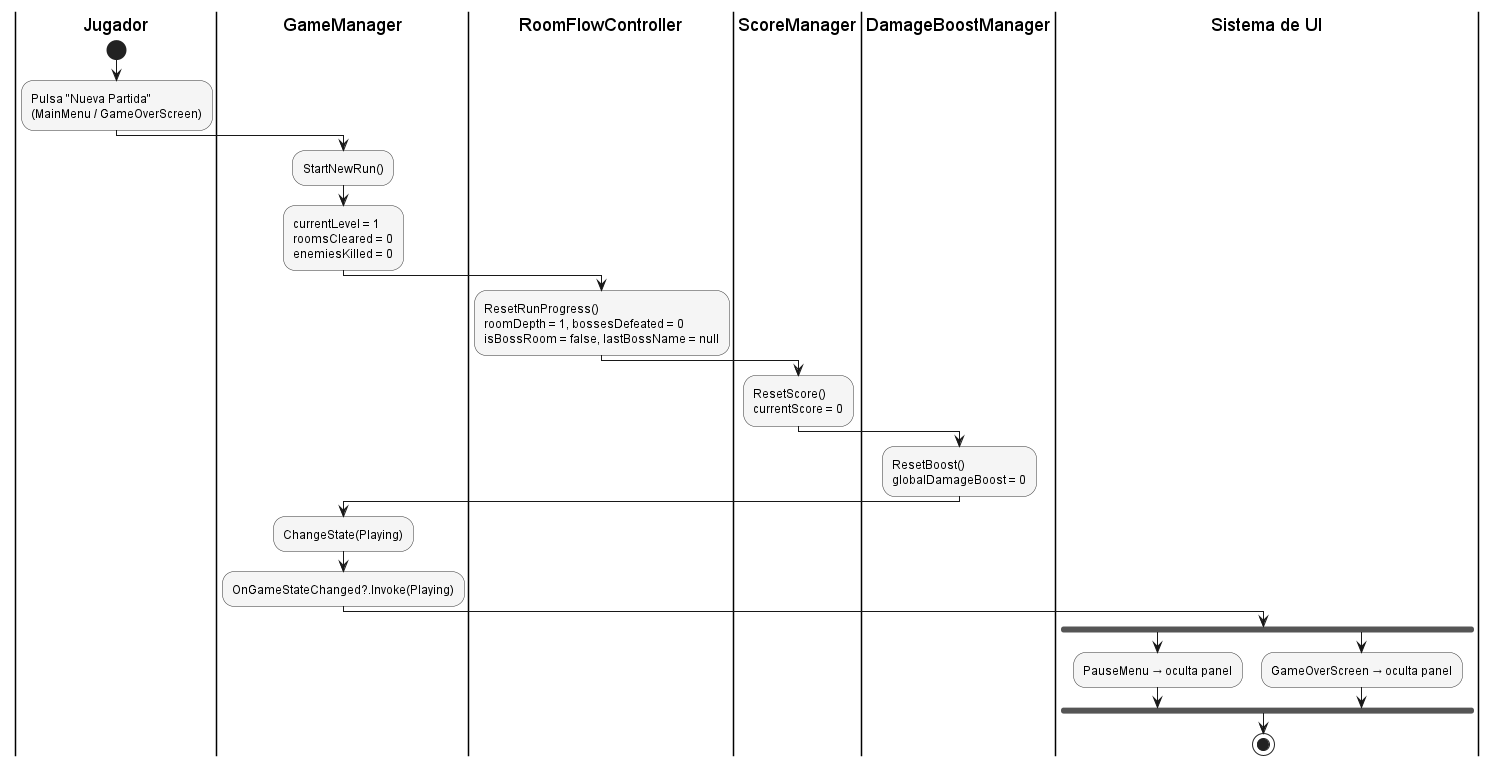
\includegraphics[width=0.95\textwidth,height=0.72\textheight,keepaspectratio]{Figuras/cadena_startnewrun.png}
\caption{
Diagrama de la coordinación entre gestores al iniciar una nueva partida. \textit{Elaboración propia.}
}
\label{fig:placeholder-2}
\end{center}
\end{figure}


\textbf{Sistema de progresión.} La puntuación se calcula según las siguientes reglas: 100 puntos por cada sala completada, una cantidad variable por cada enemigo eliminado (calculada como el daño base del enemigo multiplicado por 5), y una bonificación de 1.000 puntos en caso de completar el juego con victoria.

\textbf{Notificación de sala completada y eliminación de enemigo.} Los métodos \texttt{NotifyRoomCleared()} y \texttt{NotifyEnemyKilled()} completan el ciclo de coordinación entre el \texttt{GameManager} y los subsistemas dependientes:

\begin{lstlisting}
public void NotifyRoomCleared() {
    roomsCleared++;
    ScoreManager.Instance?.Add(100);         // 100 puntos por sala
    OnRoomCleared?.Invoke(roomsCleared);     // Notifica a RoomFlowController y UI
}

public void NotifyEnemyKilled(int scoreValue = 10) {
    enemiesKilled++;
    ScoreManager.Instance?.Add(scoreValue);  // Puntos = dano del enemigo  5
    OnEnemyKilled?.Invoke(enemiesKilled);    // Actualiza contadores de UI
}
\end{lstlisting}


El flujo completo de una sala -- desde la aparición de enemigos hasta la transición a la siguiente sala -- involucra la siguiente cadena de invocaciones entre gestores:

\begin{figure}[H]
\begin{center}
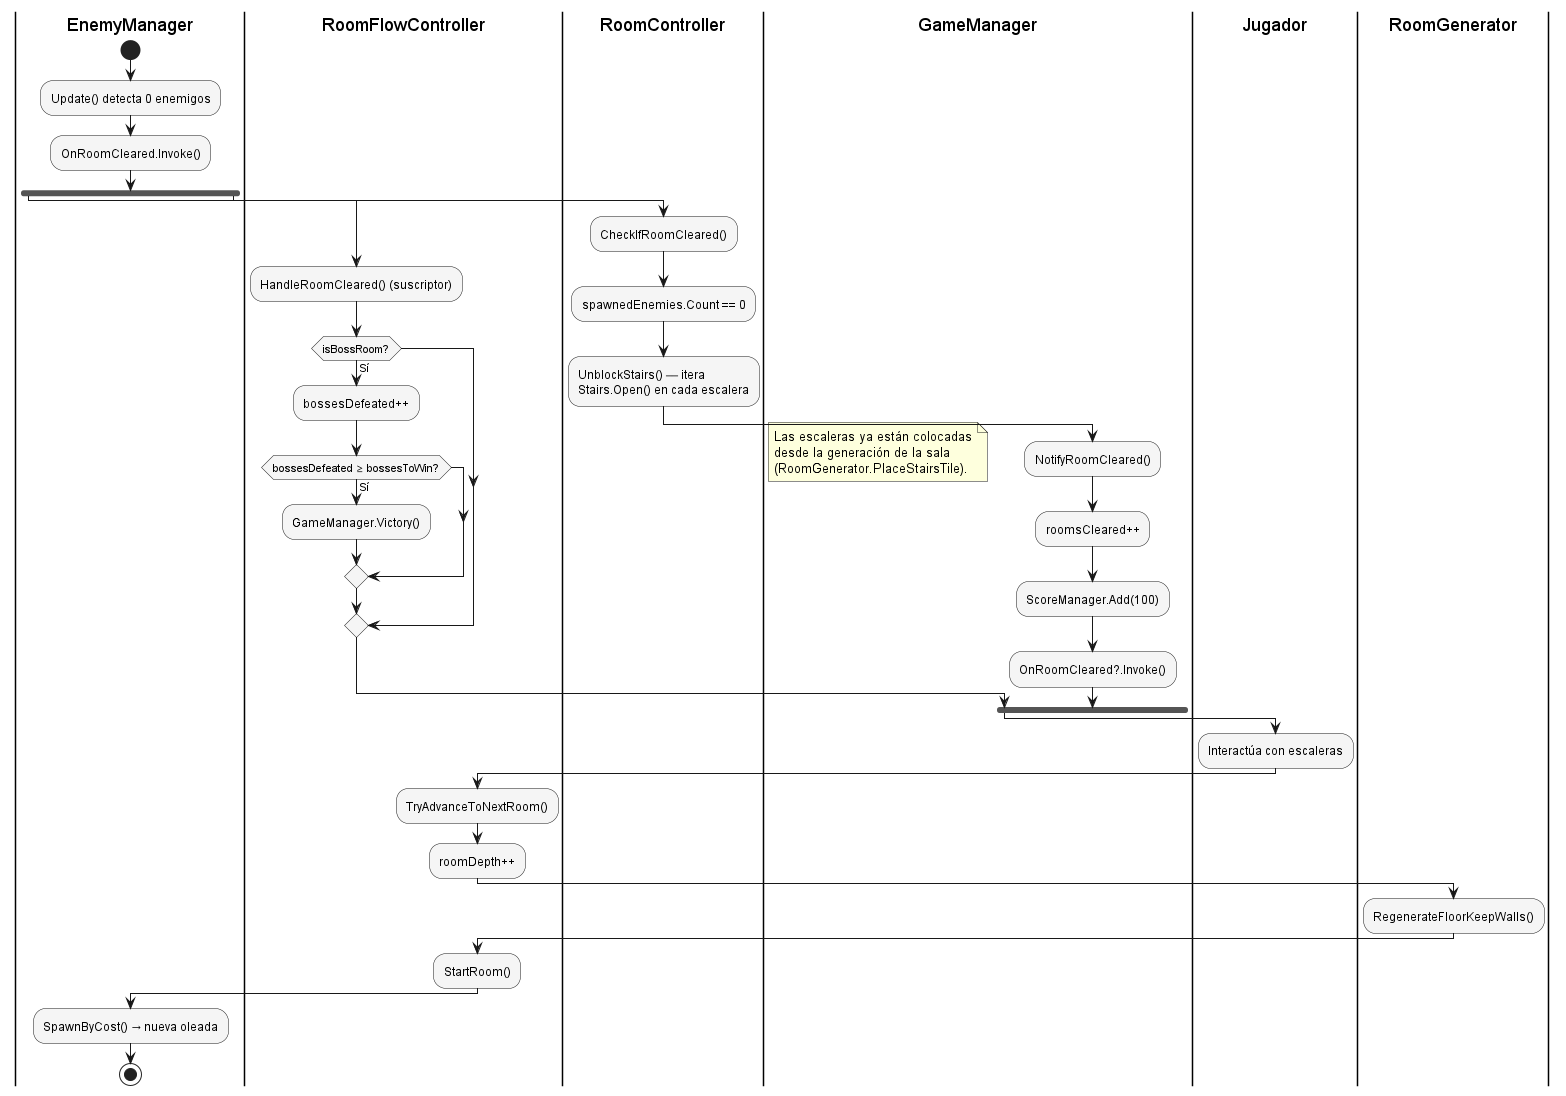
\includegraphics[width=0.95\textwidth,height=0.72\textheight,keepaspectratio]{Figuras/flujo_completar_sala.png}
\caption{
Diagrama del flujo de completar una sala. \textit{Elaboración propia.}
}
\label{fig:placeholder-3}
\end{center}
\end{figure}


\begin{figure}[H]
\begin{center}
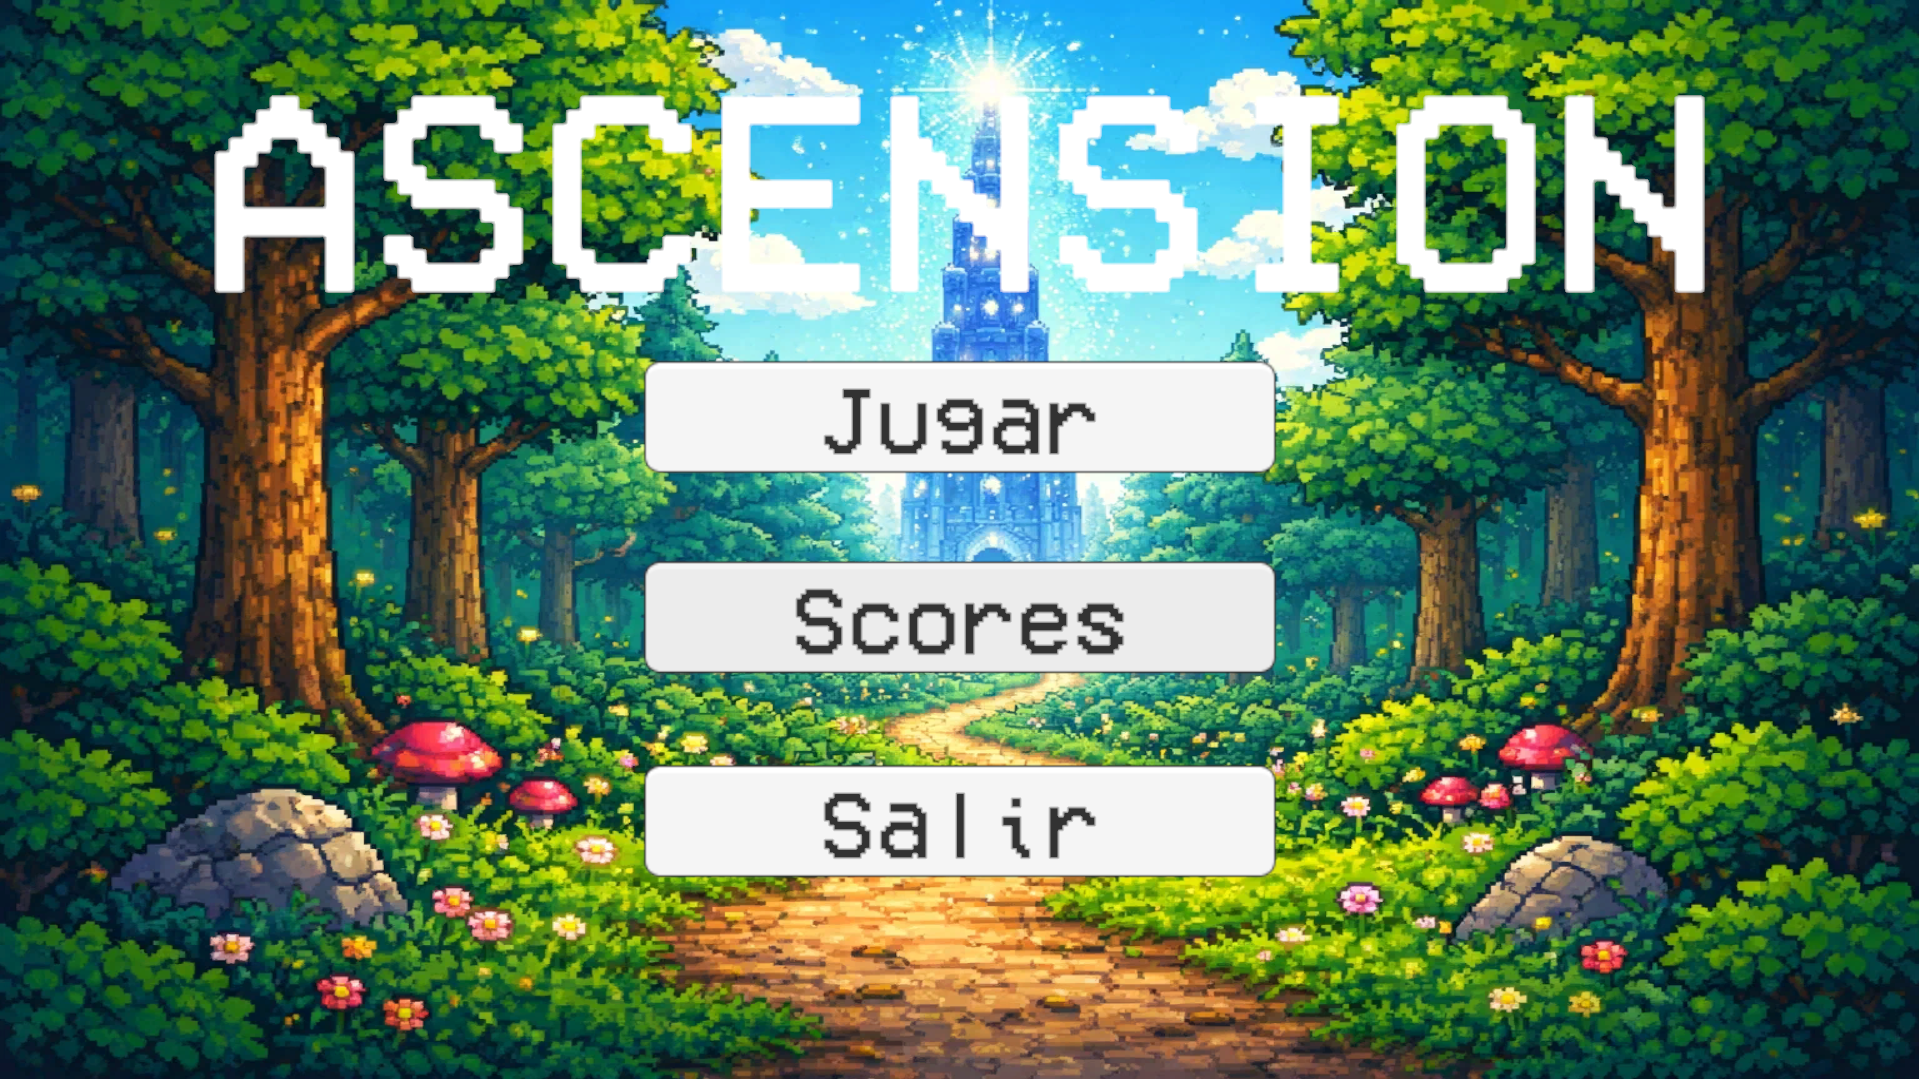
\includegraphics[width=0.9\textwidth]{Figuras/Main_Menu.png}
\caption{Captura de pantalla del menú principal de \textit{Ascension}, mostrando las opciones de nueva partida, tabla de puntuaciones y salir. \textit{Elaboración propia.}}
\label{fig:placeholder-4}
\end{center}
\end{figure}


\subsection{RoomFlowController: control de progresión de salas}


El \texttt{RoomFlowController} gestiona el bucle central de generación y progresión de salas. Su ciclo de funcionamiento se describe mediante el siguiente diagrama:

\begin{figure}[H]
\begin{center}
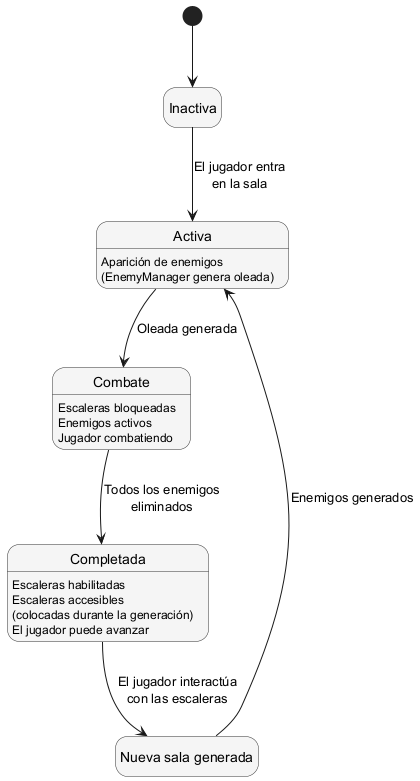
\includegraphics[width=0.95\textwidth,height=0.72\textheight,keepaspectratio]{Figuras/estados_sala.png}
\caption{
Diagrama del ciclo de funcionamiento de generación de salas. \textit{Elaboración propia.}
}
\label{fig:placeholder-5}
\end{center}
\end{figure}


\textbf{Sistema de jefes periódicos.} Cada cinco salas completadas, la siguiente sala contiene un enemigo jefe en lugar de una oleada estándar. En este proyecto, un “jefe” no introduce una IA completamente nueva, sino que se define como una \textbf{variante del enemigo base con atributos incrementados} (\textit{escalado}): mayor tamaño visual (multiplicador de escala de $2{,}4\times$) y mayor resistencia (multiplicador de vida de ocho veces). Este enfoque permite introducir picos de dificultad de forma controlada sin añadir un subsistema adicional de IA de jefes.
\begin{itemize}
\item Jefe 1: Slime verde (francotirador) escalado
\item Jefe 2: Slime rojo (perseguidor) escalado
\item Jefe 3: Slime azul (saltador) escalado
\end{itemize}

\subsection{ScoreManager: sistema de puntuación y persistencia}


El \texttt{ScoreManager} implementa la persistencia de datos de partidas mediante \texttt{PlayerPrefs} y serialización JSON. \texttt{PlayerPrefs} es un mecanismo de almacenamiento local simple (pares clave–valor) proporcionado por Unity, adecuado para guardar preferencias y pequeños volúmenes de datos. La serialización a JSON convierte las estructuras del historial en texto estructurado para poder almacenarlas y recuperarlas de forma consistente entre ejecuciones del juego. Cada entrada del historial almacena la siguiente información:

\begin{lstlisting}
public class ScoreEntry {
    public long utcTicks;        // Marca de tiempo
    public int score;            // Puntuacion final
    public int roomsCleared;     // Salas completadas
    public int enemiesKilled;    // Enemigos eliminados
    public string playerClass;   // Clase utilizada
    public string result;        // "Victory" o "GameOver"
}
\end{lstlisting}


El historial se limita a un máximo de 30 entradas, realizando limpieza automática de las entradas más antiguas cuando se alcanza este límite. Los datos se persisten entre sesiones de juego mediante su serialización a formato JSON y su almacenamiento en \texttt{PlayerPrefs}.



\section{Sistema del jugador}


\textbf{Evolución iterativa.} El sistema del jugador experimentó ajustes relevantes durante el desarrollo. La primera implementación del movimiento utilizaba \texttt{GetAxis} (con suavizado) en lugar de \texttt{GetAxisRaw}, lo que generaba una latencia perceptible entre la pulsación de tecla y el inicio del movimiento; las sesiones de juego revelaron que esta latencia era inadecuada para un \textit{roguelike} de acción, y se sustituyó por \texttt{GetAxisRaw}. El sistema de esquiva (\textit{roll}) se incorporó en una iteración posterior a la implementación del sistema de enemigos: las primeras pruebas de combate demostraron que el jugador carecía de opciones defensivas activas, ya que la única forma de evitar daño era el movimiento. La invulnerabilidad post-daño (parpadeo a 12 Hz) se añadió tras detectar que los enemigos podían infligir varios impactos en fotogramas consecutivos, resultando en muertes instantáneas que el jugador percibía como injustas.

\subsection{PlayerController: control de movimiento}


El \texttt{PlayerController} gestiona el movimiento del personaje, la habilidad de esquiva y la inicialización basada en la clase seleccionada. El sistema de movimiento soporta ocho direcciones y normaliza el vector resultante para evitar que el movimiento diagonal sea más rápido que el movimiento en ejes cardinales:

\begin{lstlisting}
void Update() {
    if (isRolling) return;
    float hor = Input.GetAxisRaw("Horizontal");
    float ver = Input.GetAxisRaw("Vertical");
    velocity = new Vector3(hor, ver, 0).normalized * speed;
    if (canRoll && Input.GetKeyDown(rollKey)) {
        Vector2 rollDir = new Vector2(hor, ver).normalized;
        StartCoroutine(DoRoll(rollDir));
    }
}

void FixedUpdate() {
    if (!isRolling && rigidbody != null) {
        rigidbody.MovePosition(rigidbody.position + (Vector2)(velocity * Time.fixedDeltaTime));
    }
}
\end{lstlisting}


Línea por línea:

\begin{itemize}
\item \textbf{Línea 1:} Si el jugador está ejecutando una esquiva, se ignora toda la entrada de movimiento; el \textit{roll} tiene su propia lógica de velocidad gestionada por la corutina.
\item \textbf{Líneas 2-3:} \texttt{GetAxisRaw} devuelve -1, 0 o 1 sin suavizado de transición, lo que produce un movimiento inmediato y responsivo. Se seleccionó \texttt{GetAxisRaw} frente a \texttt{GetAxis} porque este último aplica un suavizado temporal que introduce latencia perceptible entre la pulsación de tecla y el movimiento, inadecuado para un \textit{roguelike} de acción en tiempo real donde la precisión de movimiento es crítica.
\item \textbf{Línea 4:} \texttt{.normalized} convierte el vector a magnitud 1 antes de multiplicar por \texttt{speed}. Esta normalización resuelve un problema clásico de los videojuegos 2D: sin ella, el movimiento diagonal (por ejemplo, W+D) tendría magnitud $\sqrt{2} \approx 1{,}41$, lo que haría al personaje un 41 \% más rápido en diagonal que en ejes cardinales.
\item \textbf{Líneas 5-7:} La esquiva solo se activa si el jugador puede esquivar (\texttt{canRoll}) y si la tecla se pulsa (\texttt{GetKeyDown}, no \texttt{GetKey}). La dirección del \textit{roll} se calcula a partir de la entrada actual, y se inicia la corutina \texttt{DoRoll(rollDir)} que gestiona la velocidad, la invulnerabilidad y la travesía de colisiones.
\item \textbf{Líneas 8-10:} La aplicación de movimiento se realiza en \texttt{FixedUpdate()} mediante \texttt{MovePosition}, que desplaza al jugador basándose en la velocidad calculada multiplicada por \texttt{fixedDeltaTime}. Se utiliza \texttt{MovePosition} en lugar de asignar \texttt{linearVelocity} porque este método respeta la interpolación del \texttt{Rigidbody2D} y produce un movimiento más suave. \texttt{FixedUpdate()} se ejecuta a una frecuencia fija (50 Hz de forma predeterminada) independiente de la tasa de fotogramas.
\end{itemize}

\textbf{Inicialización basada en clase.} Al instanciar al jugador, el \texttt{PlayerController} recibe un \textit{ScriptableObject} de tipo \texttt{PlayerClass} que define las estadísticas iniciales del personaje y el arma con la que comienza la partida:

\begin{lstlisting}
public void Initialize() {
    baseSpeed = playerClass.speed;
    speed = baseSpeed;
    
    // Instanciar arma inicial
    GameObject weaponInstance = Instantiate(
        playerClass.startingWeaponData.weaponPrefab,
        transform.position,
        Quaternion.identity,
        transform
    );
    
    // Inicializar script del arma
    Weapon weaponScript = weaponInstance.GetComponent<Weapon>();
    weaponScript.weaponData = playerClass.startingWeaponData;
    weaponScript.Initialize();
}
\end{lstlisting}


Este diseño permite añadir nuevas clases de personaje sin modificar el código del \textit{controller}, ya que toda la configuración se define en activos de tipo \textit{ScriptableObject} editables desde el inspector de Unity.

\textbf{Sistema de esquiva (\textit{roll}).} La mecánica de esquiva se implementa mediante una corutina que aplica un multiplicador de velocidad temporal, activa la invulnerabilidad del jugador y desactiva las colisiones con enemigos y proyectiles durante un periodo configurable. Al finalizar la esquiva, el sistema restaura los valores originales de velocidad, vulnerabilidad y colisiones:

\begin{figure}[H]
\begin{center}
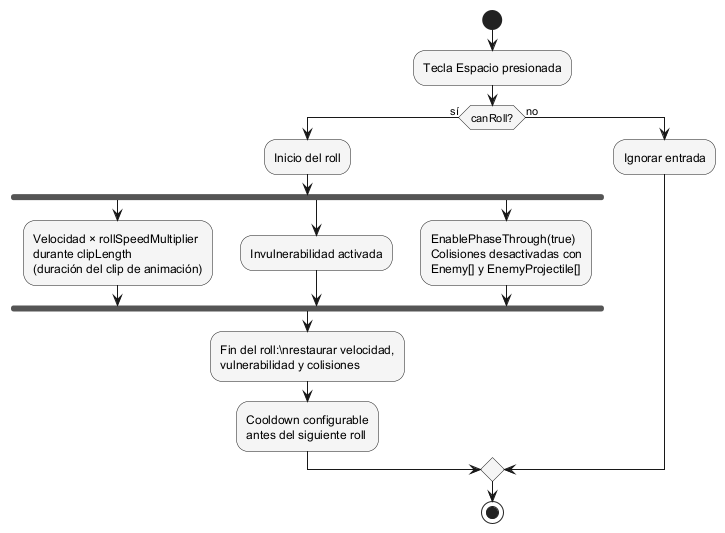
\includegraphics[width=0.95\textwidth,height=0.72\textheight,keepaspectratio]{Figuras/mecanica_esquiva.png}
\caption{
Diagrama del funcionamiento de la esquiva. \textit{Elaboración propia.}
}
\label{fig:placeholder-6}
\end{center}
\end{figure}


\textbf{Travesía de colisiones (\textit{phase-through}).} Durante la esquiva, el jugador atraviesa a los enemigos y sus proyectiles. El método \texttt{EnablePhaseThrough} utiliza \texttt{Physics2D.IgnoreCollision} de Unity para desactivar selectivamente las colisiones entre el colisionador del jugador y los de cada enemigo y proyectil enemigo activos en la escena:

\begin{lstlisting}
private void EnablePhaseThrough(bool enable) {
    Collider2D playerCollider = GetComponent<Collider2D>();
    if (playerCollider == null) return;
    
    Enemy[] enemies = FindObjectsByType<Enemy>(FindObjectsSortMode.None);
    foreach (Enemy enemy in enemies) {
        if (enemy != null) {
            Collider2D enemyCollider = enemy.GetComponent<Collider2D>();
            if (enemyCollider != null)
                Physics2D.IgnoreCollision(playerCollider, enemyCollider, enable);
        }
    }
    
    EnemyProjectile[] projectiles = FindObjectsByType<EnemyProjectile>(FindObjectsSortMode.None);
    foreach (EnemyProjectile proj in projectiles) {
        if (proj != null) {
            Collider2D projCollider = proj.GetComponent<Collider2D>();
            if (projCollider != null)
                Physics2D.IgnoreCollision(playerCollider, projCollider, enable);
        }
    }
}
\end{lstlisting}


Se seleccionó \texttt{Physics2D.IgnoreCollision} frente a la alternativa de cambiar la capa del jugador (\textit{layer}) durante la esquiva, porque el cambio de capa afectaría a todas las interacciones del jugador (incluidas paredes y tiles), mientras que \texttt{IgnoreCollision} permite desactivar selectivamente solo las colisiones con enemigos y proyectiles, manteniendo intactas las colisiones con el entorno.

\subsection{PlayerHealth: sistema de vida}


El \texttt{PlayerHealth} gestiona los puntos de vida del jugador, el sistema de invulnerabilidad temporal tras recibir daño y la detección de muerte. El método principal de recepción de daño ilustra el flujo completo:

\begin{lstlisting}
public void TakeDamage(int amount) {
    if (isInvulnerable || (playerController != null && playerController.IsInvulnerable()))
        return;
    
    currentHealth -= amount;
    currentHealth = Mathf.Clamp(currentHealth, 0, maxHealth);
    
    UpdateHearts();
    
    if (currentHealth <= 0) {
        Die();
    } else {
        if (damageCoroutine != null)
            StopCoroutine(damageCoroutine);
        damageCoroutine = StartCoroutine(DamageInvulnerabilityCoroutine());
    }
}
\end{lstlisting}


La verificación inicial comprueba si el jugador se encuentra en estado de invulnerabilidad, ya sea por haber recibido daño previamente (invulnerabilidad temporal) o por estar ejecutando una esquiva; la comprobación \texttt{playerController != null} previene errores si la referencia aún no está inicializada. La función \texttt{Mathf.Clamp} evita que la vida descienda por debajo de cero o exceda el máximo. Tras actualizar la representación visual de los corazones, se evalúa si el jugador ha muerto; en caso contrario, se cancela cualquier corutina de parpadeo en curso (\texttt{damageCoroutine}) antes de iniciar una nueva, evitando conflictos visuales cuando el jugador recibe impactos consecutivos.

\textbf{Efecto visual de parpadeo.} Durante el periodo de invulnerabilidad, el sprite del jugador parpadea alternando entre su color original y blanco, y opcionalmente alternando su visibilidad, a una frecuencia configurable (de forma predeterminada, doce Hz). Si existe una corutina de parpadeo anterior en curso, se cancela antes de iniciar la nueva para evitar conflictos:

\begin{lstlisting}
private IEnumerator DamageInvulnerabilityCoroutine() {
    isInvulnerable = true;

    if (spriteRenderers == null || spriteRenderers.Length == 0)
        CacheSpriteRenderers();

    float end = Time.time + Mathf.Max(0f, invulnerableTime);
    float blinkPeriod = blinkFrequencyHz > 0f ? (1f / blinkFrequencyHz) : 0.1f;
    float nextToggle = 0f;
    bool white = true;
    bool visible = true;

    while (Time.time < end) {
        if (Time.time >= nextToggle) {
            nextToggle = Time.time + blinkPeriod;
            white = !white;
            visible = !visible;
        }

        for (int i = 0; i < spriteRenderers.Length; i++) {
            var sr = spriteRenderers[i];
            if (sr == null) continue;
            sr.enabled = visibilityBlinkOnDamage ? visible : true;
            sr.color = white ? Color.white : originalColors[i];
        }

        yield return null;
    }

    for (int i = 0; i < spriteRenderers.Length; i++) {
        if (spriteRenderers[i] == null) continue;
        spriteRenderers[i].color = originalColors[i];
        spriteRenderers[i].enabled = true;
    }

    isInvulnerable = false;
    damageCoroutine = null;
}
\end{lstlisting}


La instrucción \texttt{yield return null} cede la ejecución hasta el siguiente fotograma sin bloquear el hilo principal del juego. El final del efecto se controla comparando \texttt{Time.time} (tiempo global del juego) con el instante \texttt{end}, lo que permite que la duración de la invulnerabilidad sea consistente independientemente de la tasa de fotogramas.

El cambio de color y visibilidad se aplica a todos los \texttt{SpriteRenderer} del jugador (incluidos los de sus objetos hijos, almacenados en caché por \texttt{CacheSpriteRenderers()}) para que el parpadeo afecte al personaje completo. La variable \texttt{visibilityBlinkOnDamage} permite alternar no solo el color, sino también la visibilidad (\texttt{sr.enabled}) de cada renderer, produciendo un efecto de parpadeo más notorio. Al finalizar la corutina, se restablece el estado original de todos los renderers y se marca \texttt{damageCoroutine = null} para permitir la gestión correcta de corutinas superpuestas.

\subsubsection{Diagrama del ciclo de vida del jugador}


El ciclo de vida del jugador integra los subsistemas de movimiento (\texttt{PlayerController}), vida (\texttt{PlayerHealth}) y esquiva, atravesando los siguientes estados durante una partida:

\begin{figure}[H]
\begin{center}
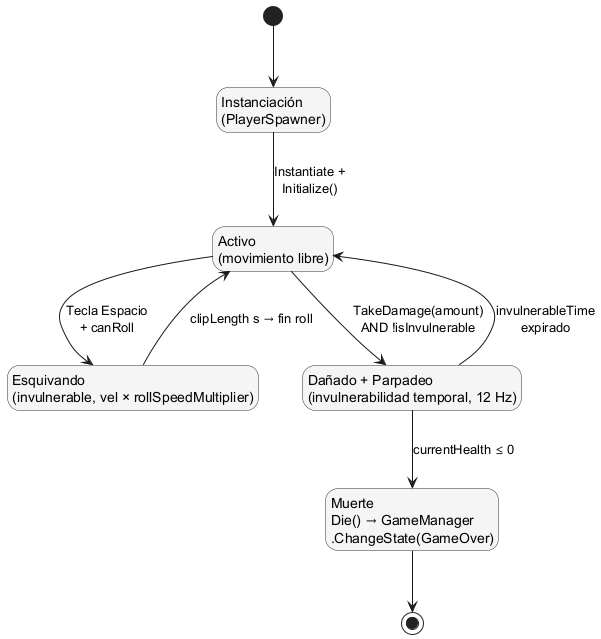
\includegraphics[width=0.95\textwidth,height=0.72\textheight,keepaspectratio]{Figuras/ciclo_vida_jugador.png}
\caption{
Ciclo de vida del jugador. \textit{Elaboración propia.}
}
\label{fig:placeholder-7}
\end{center}
\end{figure}


Este diagrama muestra que el jugador solo puede recibir daño en el estado \textbf{Activo} (ni durante la esquiva ni durante la invulnerabilidad post-daño), lo que proporciona dos mecanismos de protección distintos: uno proactivo (esquiva voluntaria) y otro reactivo (invulnerabilidad automática tras daño). Cuando la vida alcanza cero, se ejecuta un parpadeo rojo rápido (cinco alternancias rojo/blanco a 0,08 s por cambio, duración total de 0,8 s) que proporciona retroalimentación visual de muerte antes de notificar al \texttt{GameManager} para que transite al estado \texttt{GameOver}, ejemplificando la interacción \textit{Observer} + \textit{State Machine} descrita en el capítulo de diseño.

\subsection{PlayerSpawner: instanciación del jugador}


El \texttt{PlayerSpawner} se encarga de instanciar al jugador al inicio de la escena de juego, aplicando la clase seleccionada en la escena anterior:

\begin{lstlisting}
void Start() {
    if (ClassSelectionManager.SelectedClass == null) {
        Debug.LogError("No se ha seleccionado ninguna clase.");
        SceneManager.LoadScene("ClassSelection");
        return;
    }
    
    GameObject player = Instantiate(
        playerPrefab, 
        spawnPoint.position, 
        Quaternion.identity
    );
    
    var controller = player.GetComponent<PlayerController>();
    controller.playerClass = ClassSelectionManager.SelectedClass;
    controller.Initialize();
}
\end{lstlisting}


Si el jugador accede a la escena de juego sin haber seleccionado una clase -- por ejemplo, durante la depuración --, el sistema detecta esta situación y redirige automáticamente a la escena de selección.

\subsection{PlayerClass: datos de configuración mediante \textit{ScriptableObjects}}


Los datos de cada clase de personaje se definen mediante un \textit{ScriptableObject}. Se seleccionó este mecanismo frente a dos alternativas: (a) codificar las estadísticas directamente en variables del \texttt{PlayerController}, lo que obligaría a duplicar y recompilar el script para cada combinación de parámetros; y (b) cargar los datos desde un fichero externo (JSON o XML), lo que añadiría lógica de lectura, deserialización y validación sin integración con el inspector de Unity.

El \textit{ScriptableObject} resuelve ambos problemas: es un activo nativo del proyecto que se edita directamente desde el inspector, se serializa automáticamente con el proyecto, y se vincula al \texttt{PlayerController} mediante una referencia en el campo \texttt{playerClass}. Esta decisión tiene una implicación arquitectónica directa: para añadir una nueva clase de personaje, basta con crear un nuevo activo de tipo \texttt{PlayerClass} desde el menú del editor (\texttt{Roguelike/PlayerClass}), configurar sus estadísticas y asignarle un arma inicial, sin modificar una sola línea del código del \texttt{PlayerController}.

\begin{lstlisting}
[CreateAssetMenu(fileName = "PlayerClass", menuName = "Roguelike/PlayerClass")]
public class PlayerClass : ScriptableObject {
    public string className;        // Nombre visible de la clase (p. ej., "Guerrero")
    public int maxHealth = 5;       // Puntos de vida maximos
    public float speed = 32f;       // Velocidad base en unidades/segundo
    public WeaponData startingWeaponData;  // Referencia al arma inicial (otro ScriptableObject)
}
\end{lstlisting}


Línea por línea:

\begin{itemize}
\item \texttt{[CreateAssetMenu(...)]}: atributo de Unity que añade una entrada al menú contextual del editor, permitiendo crear instancias de este \textit{ScriptableObject} directamente desde \texttt{Assets > Create > Roguelike > PlayerClass}.
\item \texttt{className}: cadena que identifica la clase en la interfaz de usuario (pantalla de selección y estadísticas finales).
\item \texttt{maxHealth = 5}: valor predeterminado que diferencia las clases; el guerrero podría tener 7 y el mago 3.
\item \texttt{speed = 32f}: velocidad base en unidades del mundo por segundo; a 16 PPU (píxeles por unidad), equivale a 512 píxeles por segundo.
\item \texttt{startingWeaponData}: referencia a otro \textit{ScriptableObject} (\texttt{WeaponData}) que define el arma con la que la clase comienza la partida. Esta composición de \textit{ScriptableObjects} permite que la misma arma pueda reutilizarse en múltiples clases sin duplicar datos.
\end{itemize}

\section{Sistema de enemigos}


\textbf{Evolución iterativa.} El sistema de enemigos fue el subsistema que más iteraciones requirió. Inicialmente, cada tipo de enemigo se implementó como una clase independiente sin herencia compartida, lo que provocó duplicación de la lógica de vida, daño y muerte en tres archivos. La refactorización hacia la jerarquía con \textit{Template Method} (clase base \texttt{Enemy} + subclases) se realizó en la cuarta iteración del módulo. El sistema de periodos de gracia (\texttt{contactDamageGraceSeconds}, \texttt{aiGraceSeconds}) se descubrió durante las pruebas de juego: sin este mecanismo, los enemigos dañaban al jugador en el fotograma de aparición. El limitador de velocidad (\texttt{CapToPlayerSpeed}) surgió de la misma forma: el SlimeGreen en estado de huida se movía más rápido que el jugador, haciendo imposible la persecución. Ambos mecanismos se integraron en la clase base \texttt{Enemy} para que todos los tipos de enemigo los heredasen automáticamente.

\subsection{Enemy: clase base y patrón \textit{Template Method}}


La clase \texttt{Enemy} define el comportamiento base compartido por todos los tipos de enemigo del juego. Se seleccionó el patrón \textit{Template Method} frente a la alternativa de implementar cada enemigo como una clase independiente sin herencia. Esta alternativa se descartó porque los tres tipos de enemigo comparten un núcleo de funcionalidad significativo: gestión de puntos de vida (recepción de daño, muerte), periodos de gracia tras la aparición, interacción con tiles de velocidad, detección de contacto con el jugador y notificación al \texttt{GameManager} al morir. Duplicar esta lógica en tres clases independientes habría generado aproximadamente 180 líneas de código redundante y habría introducido riesgo de inconsistencias: si se modificase la lógica de daño en un tipo de enemigo pero no en los demás, se producirían discrepancias difíciles de detectar.

El \textit{Template Method} resuelve este problema: la clase base \texttt{Enemy} define el esqueleto de comportamiento común, y cada subclase sobrescribe exclusivamente el método \texttt{Update()} para definir su IA específica.

\textbf{Sistema de gracia al aparecer.} Para evitar que los enemigos ataquen al jugador inmediatamente tras aparecer -- lo que resultaría en una experiencia injusta --, se implementa un sistema de periodos de gracia:

\begin{lstlisting}
[SerializeField] private float contactDamageGraceSeconds = 0.75f;
[SerializeField] private float aiGraceSeconds = 0.75f;

protected bool IsAIEnabled => Time.time >= aiEnabledTime;
\end{lstlisting}


En este contexto, \texttt{Time.time} representa el tiempo transcurrido desde el inicio de la ejecución del juego. La IA se habilita cuando dicho tiempo supera un instante programado (\texttt{aiEnabledTime}), de modo que el enemigo “espera” un breve intervalo antes de comenzar a actuar.

Durante los primeros 0,75 segundos tras su aparición, el enemigo no puede infligir daño por contacto ni ejecutar su lógica de inteligencia artificial. Este intervalo proporciona al jugador una ventana de reacción justa.

\textbf{Interacción con tiles de velocidad.} Los enemigos, al igual que el jugador, se ven afectados por los tiles de velocidad del suelo:

\begin{lstlisting}
public void SetTileSpeedMultiplier(float multiplier) {
    tileSpeedMultiplier = Mathf.Clamp(multiplier, 0.1f, 5f);
}
\end{lstlisting}


Esta mecánica añade profundidad táctica al combate, ya que el jugador puede utilizar las zonas de lodo para ralentizar a los enemigos perseguidores o las zonas de hielo para alejarse rápidamente.

\textbf{Sistema de muerte.} Al alcanzar cero puntos de vida, el enemigo notifica al \texttt{GameManager} para el cálculo de puntuación y ejecuta un parpadeo rojo de retroalimentación visual antes de destruirse:

\begin{lstlisting}
protected virtual void Die() {
    if (isDead) return;
    isDead = true;

    if (rb != null) {
        rb.linearVelocity = Vector2.zero;
        rb.bodyType = RigidbodyType2D.Kinematic;
    }
    if (animator != null)
        animator.enabled = false;
    
    if (GameManager.Instance != null) {
        int scoreValue = enemyData != null ? enemyData.damage * 5 : 10;
        GameManager.Instance.NotifyEnemyKilled(scoreValue);
    }

    StartCoroutine(DeathBlinkCoroutine());
}

private IEnumerator DeathBlinkCoroutine() {
    int blinks = 4;
    float interval = 0.08f;

    for (int i = 0; i < blinks; i++) {
        SetSpriteRenderersColor(Color.red);
        yield return new WaitForSeconds(interval);
        SetSpriteRenderersColor(Color.white);
        yield return new WaitForSeconds(interval);
    }

    if (animator != null && animator.runtimeAnimatorController != null && hasAnimDieTrigger) {
        animator.enabled = true;
        animator.SetTrigger("Die");
        Destroy(gameObject, 0.5f);
    } else {
        Destroy(gameObject);
    }
}
\end{lstlisting}


Antes de notificar al \texttt{GameManager}, el método \texttt{Die()} congela al enemigo: se anula la velocidad del \texttt{Rigidbody2D} y se cambia su tipo a \texttt{Kinematic} para impedir que la física lo desplace (incluido el \textit{dash} del SlimeBlue, cuyo \texttt{FixedUpdate} sigue asignando velocidad mientras \texttt{isDashing} sea verdadero). Además, se desactiva el \texttt{Animator} para que el sprite quede estático mirando hacia la última dirección, evitando que la animación de movimiento continúe durante el parpadeo. La corutina \texttt{DeathBlinkCoroutine()} alterna el color de todos los \texttt{SpriteRenderer} entre rojo y blanco cuatro veces (intervalo de 0,08 s por cambio, duración total de 0,64 s), proporcionando retroalimentación visual inmediata de eliminación. Tras el parpadeo, si el \texttt{Animator} dispone de un trigger \texttt{Die}, se reactiva para reproducir la animación de muerte y el objeto se destruye tras 0,5 s; en caso contrario, se destruye inmediatamente.

\textbf{Daño por contacto.} Los enemigos infligen daño continuo al jugador mientras permanecen en contacto con él, verificado mediante \texttt{OnCollisionStay2D}. El sistema respeta tanto el periodo de gracia al aparecer como el estado de esquiva del jugador:

\begin{lstlisting}
protected virtual void OnCollisionStay2D(Collision2D collision) {
    if (isDead) return;
    
    if (collision.gameObject.CompareTag("Player")) {
        PlayerController pc = collision.gameObject.GetComponent<PlayerController>();
        if (pc != null && pc.IsRolling) return;          // Sin dano durante roll
        
        if (Time.time < contactDamageEnabledTime) return; // Periodo de gracia
        
        if (Time.time >= lastDamageTime + damageRate) {
            PlayerHealth ph = collision.gameObject.GetComponent<PlayerHealth>();
            if (ph != null && enemyData != null) {
                ph.TakeDamage(enemyData.damage);
                lastDamageTime = Time.time;
            }
        }
    }
}
\end{lstlisting}


La comprobación \texttt{pc.IsRolling} conecta el sistema de contacto con la mecánica de esquiva documentada anteriormente: durante la ejecución de un \textit{roll}, el jugador no recibe daño por contacto, proporcionando un uso defensivo a la mecánica de esquiva.

\subsection{SlimeGreen: enemigo francotirador}


El \texttt{SlimeGreen} implementa un comportamiento de combate a distancia. Se diseñó este arquetipo para obligar al jugador a adoptar una postura ofensiva: frente a un enemigo que huye al ser perseguido, el jugador no puede limitarse a esquivar, sino que debe cerrar la distancia activamente o utilizar armas a distancia. La alternativa descartada era crear un segundo enemigo perseguidor con estadísticas diferentes, pero esto habría reducido la variedad táctica al ofrecer el mismo tipo de desafío con números distintos.

Su inteligencia artificial sigue un patrón de \textbf{máquina de estados finitos (FSM) implícita con tres estados}, evaluados en cada fotograma mediante la distancia euclidiana al jugador. Aunque los estados no se representan como una enumeración explícita en el código -- a diferencia del \texttt{GameState} del \texttt{GameManager} --, el comportamiento resultante es funcionalmente equivalente a una FSM formal. La siguiente tabla define los estados, las condiciones de transición y las acciones asociadas:

\begin{table}[H]
\begin{center}
\small
\begin{tabular}{|p{0.23\textwidth}|p{0.23\textwidth}|p{0.23\textwidth}|p{0.23\textwidth}|}
\hline
\textbf{Estado} & \textbf{Condición de entrada} & \textbf{Acción ejecutada} & \textbf{Transición de salida} \\ \hline
\textbf{Huida} (\textit{Escape}) & \texttt{distancia < escapeDistance} (4 u) & Movimiento en dirección opuesta al jugador a $1{,}5 \times$ velocidad base, limitado por \texttt{CapToPlayerSpeed} & -> Disparo si distancia >= 4 u; -> Acercamiento si distancia > 12 u \\ \hline
\textbf{Disparo} (\textit{Shoot}) & \texttt{escapeDistance <= distancia <= maxDistance} (4–12 u) & Detención completa (\texttt{rb.linearVelocity = Vector2.zero}) + disparo de proyectil si \texttt{Time.time >= nextShootTime} & -> Huida si distancia < 4 u; -> Acercamiento si distancia > 12 u \\ \hline
\textbf{Acercamiento} (\textit{Approach}) & \texttt{distancia > maxDistance} (12 u) & Movimiento hacia el jugador a velocidad base, limitado por \texttt{CapToPlayerSpeed} & -> Disparo si distancia <= 12 u; -> Huida si distancia < 4 u \\ \hline
\end{tabular}
\end{center}
\end{table}


\TablaTitulo{Estados, transiciones y acciones de la FSM del SlimeGreen.
}

El siguiente diagrama de estados formaliza las transiciones entre los tres estados:

\begin{figure}[H]
\begin{center}
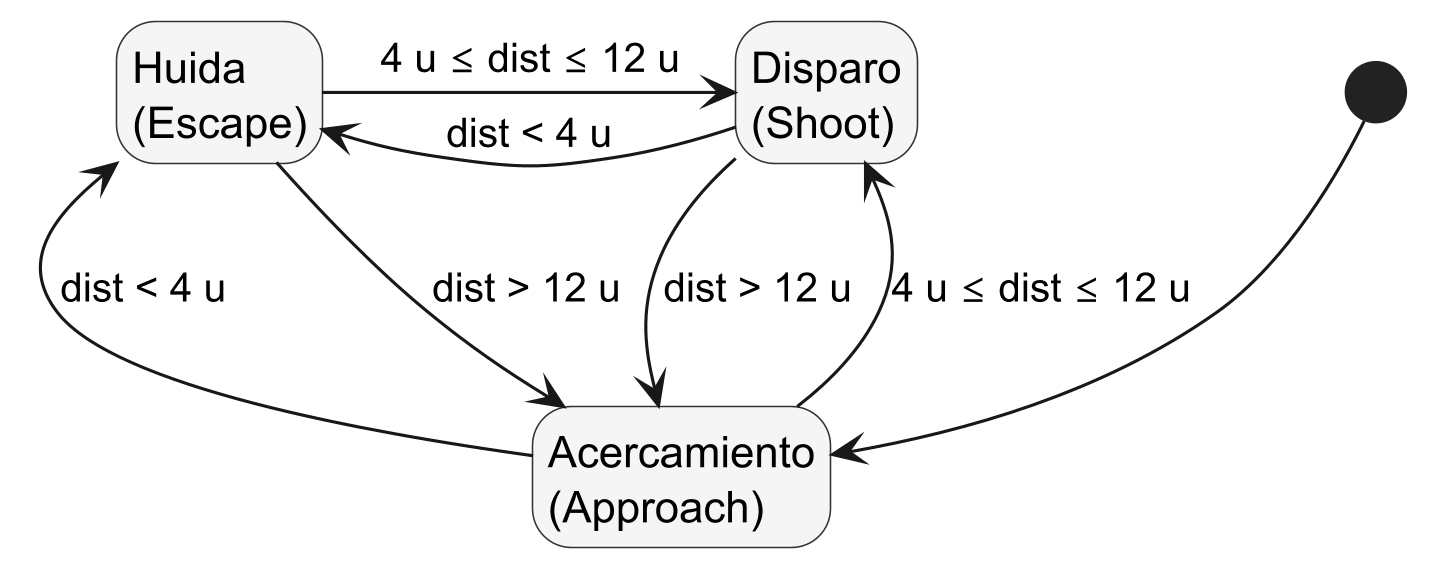
\includegraphics[width=0.95\textwidth,height=0.72\textheight,keepaspectratio]{Figuras/fsm_slimegreen.png}
\caption{
Diagrama de la FSM del SlimeGreen. \textit{Elaboración propia.}
}
\label{fig:placeholder-8}
\end{center}
\end{figure}


La implementación concreta en el método \texttt{Update()} del \texttt{SlimeGreen} muestra cómo la evaluación de distancia en cada fotograma sustituye a una tabla de transiciones explícita:

\begin{lstlisting}
protected override void Update() {
    base.Update();                                          // (1) Logica base: gracia, tiles
    
    if (isDead || player == null) return;                   // (2) Guardas de seguridad
    
    if (!IsAIEnabled) {                                     // (3) Periodo de gracia (0,75 s)
        StopMoving();
        return;
    }
    
    float distanceToPlayer = Vector2.Distance(              // (4) Distancia euclidiana
        transform.position, player.position);
    
    if (distanceToPlayer < escapeDistance) {                 // (5) FSM: transicion a Huida
        Escape();
    } else if (distanceToPlayer > maxDistance) {             // (6) FSM: transicion a Acercamiento
        Approach();
    } else {                                                // (7) FSM: estado Disparo
        StopMoving();
        if (Time.time >= nextShootTime) {
            Shoot();
        }
    }
    
    UpdateFallbackAnimation();                              // (8) Animacion procedural de respaldo
}
\end{lstlisting}


Línea por línea:

\begin{itemize}
\item \textbf{(1)} \texttt{base.Update()}: invoca el \texttt{Update()} de la clase base \texttt{Enemy}, que gestiona la interacción con tiles de velocidad y la detección de daño por contacto. Esta llamada es obligatoria en cualquier subclase que sobrescriba \texttt{Update()}, ya que sin ella los periodos de gracia y los modificadores de velocidad por tile dejarían de funcionar -- un ejemplo concreto de cómo el patrón \textit{Template Method} impone un contrato entre la clase base y las subclases.
\item \textbf{(2)} Las guardas \texttt{isDead} y \texttt{player == null} previenen la ejecución de lógica de IA sobre enemigos ya eliminados o cuando la referencia al jugador se ha perdido (por ejemplo, durante la transición de sala).
\item \textbf{(3)} \texttt{IsAIEnabled} es una propiedad de la clase base \texttt{Enemy} que compara \texttt{Time.time} con \texttt{aiEnabledTime}. Durante los primeros 0,75 segundos tras la aparición, esta propiedad devuelve \texttt{false}, y el enemigo permanece inactivo: esta ventana impide que el enemigo dispare al jugador en el mismo fotograma en que aparece.
\item \textbf{(4)} \texttt{Vector2.Distance} calcula la distancia euclidiana $d = \sqrt{(x_2 - x_1)^2 + (y_2 - y_1)^2}$ entre el enemigo y el jugador. Esta métrica se evalúa en cada fotograma (~60 veces por segundo con VSync activado), lo que produce transiciones de estado inmediatas cuando el jugador cruza un umbral de distancia.
\item \textbf{(5-7)} Las tres ramas del condicional implementan las transiciones de la FSM. La prioridad de evaluación es relevante: la condición de huida se evalúa \textit{antes} que la de disparo, garantizando que la autopreservación tiene prioridad sobre el ataque cuando el jugador está muy cerca.
\item \textbf{(8)} \texttt{UpdateFallbackAnimation()}: aplica una animación procedural de respaldo (oscilación de escala al moverse, pulso al disparar) cuando el \texttt{Animator} no dispone de un \texttt{AnimatorController} asignado. Esto garantiza retroalimentación visual incluso en configuraciones incompletas.
\end{itemize}

El comportamiento resultante es el de un enemigo que busca mantener una distancia óptima respecto al jugador: si este se acerca demasiado, el slime verde retrocede; si se aleja demasiado, el slime verde se aproxima; cuando se encuentra a la distancia ideal, se detiene y dispara proyectiles con una cadencia configurable.

\textbf{Análisis de la complejidad computacional de la FSM.} La evaluación de la FSM tiene coste $O(1)$ por fotograma: una llamada a \texttt{Vector2.Distance} (una raíz cuadrada) y tres comparaciones. Para los tres tipos de enemigo simultáneamente y una oleada típica de 8-12 enemigos, el coste total por fotograma es $O(n)$ donde $n$ es el número de enemigos activos -- despreciable frente al coste del renderizado y la simulación física.

\textbf{Sistema de disparo.} El método de disparo instancia un proyectil, le asigna una dirección calculada hacia la posición actual del jugador y le aplica una velocidad configurable. A continuación se muestra el código completo con comentarios exhaustivos:

\begin{lstlisting}
private void Shoot() {
    // Verificacion defensiva: si no hay prefab asignado, registrar advertencia
    if (projectilePrefab == null) {
        Debug.LogWarning("[SlimeGreen] No hay projectilePrefab asignado!");
        return;
    }
    
    // Calcular direccion normalizada desde el punto de disparo hacia el jugador.
    Vector2 direction = (player.position - shootPoint.position).normalized;
    
    // Instanciar proyectil en la posicion del punto de disparo,
    // sin rotacion (Quaternion.identity): la rotacion se aplica por velocidad.
    GameObject projectile = Instantiate(
        projectilePrefab, shootPoint.position, Quaternion.identity);
    
    // Aplicar multiplicadores de escala: escala de ajuste fino (20 % por defecto)
    // combinada con la escala de boss (> 1.0 para jefes).
    float finalScaleMultiplier = projectileScaleMultiplier * bossProjectileScale;
    projectile.transform.localScale *= finalScaleMultiplier;
    
    // Asignar velocidad al Rigidbody2D del proyectil.
    // Se garantiza una velocidad minima segura y se aplica el multiplicador (+15 %).
    Rigidbody2D projRb = projectile.GetComponent<Rigidbody2D>();
    float safeBaseSpeed = Mathf.Max(projectileSpeed, minProjectileBaseSpeed);
    float finalProjectileSpeed = safeBaseSpeed * projectileSpeedMultiplier;
    if (projRb != null) {
        projRb.linearVelocity = direction * finalProjectileSpeed;
    }
    
    // Asignar dano y escala externa al componente EnemyProjectile.
    EnemyProjectile projScript = projectile.GetComponent<EnemyProjectile>();
    if (projScript != null) {
        projScript.damage = projectileDamage;
        projScript.externalScaleMultiplier = finalScaleMultiplier;
    }
    
    // Actualizar la direccion del animator y activar animacion de disparo.
    SetAnimatorDirection(direction);
    TriggerShootAnimation();
    
    // Programar el siguiente disparo: Time.time + cooldown.
    nextShootTime = Time.time + shootCooldown;
}
\end{lstlisting}


\textbf{Mecánica de rebote contra muros.} Un aspecto diferenciador del SlimeGreen es su comportamiento al colisionar con los muros perimetrales durante el estado de huida. En lugar de quedarse atascado contra el muro -- lo que lo haría trivial de eliminar --, el enemigo calcula una nueva dirección de escape mediante reflexión vectorial:

\begin{lstlisting}
private void BounceFromWall(Collision2D collision) {
    if (collision.contactCount == 0) return;
    
    // Dirección deseada: alejarse del jugador
    Vector2 awayFromPlayer = (transform.position - player.position).normalized;
    // Normal de la superficie del muro en el punto de contacto
    Vector2 normal = collision.GetContact(0).normal;
    
    // Reflexión: dirección de movimiento reflejada respecto a la normal del muro
    Vector2 reflected = Vector2.Reflect(lastMoveDirection, normal).normalized;
    
    // Candidata: promedio entre la dirección de escape y la reflexión.
    Vector2 candidate = (awayFromPlayer + reflected).normalized;
    
    // Protección contra vector nulo: si el promedio se anula,
    // usar la reflexión pura o la dirección de escape como respaldo.
    if (candidate.sqrMagnitude < 0.0001f) {
        candidate = reflected.sqrMagnitude > 0.0001f ? reflected : awayFromPlayer;
    }
    
    // Corrección iterativa: si la candidata apunta hacia el jugador,
    // probar la tangente al muro como alternativa.
    for (int i = 0; i < wallBounceAttempts; i++) {
        Vector2 toPlayer = (player.position - transform.position).normalized;
        if (Vector2.Dot(candidate, toPlayer) < 0f) break;  // Ya se aleja: aceptar
        
        candidate = new Vector2(-normal.y, normal.x).normalized;
        if (Vector2.Dot(candidate, awayFromPlayer) < 0f) candidate = -candidate;
    }
    
    // Aplicar la nueva direccion
    lastMoveDirection = candidate;
    if (rb != null) {
        rb.linearVelocity = lastMoveDirection * lastAppliedMoveSpeed;
    }
}
\end{lstlisting}


Este algoritmo de rebote utiliza la fórmula de reflexión vectorial $\vec{r} = \vec{d} - 2(\vec{d} \cdot \vec{n})\vec{n}$, donde $\vec{d}$ es la dirección de movimiento y $\vec{n}$ es la normal de la superficie. La corrección iterativa garantiza que el enemigo no se dirija hacia el jugador tras el rebote, preservando la coherencia del comportamiento de huida.

\textbf{Limitador de velocidad.} Para evitar que ningun enemigo pueda ser mas rapido que el jugador -- lo que haria imposible la evasion --, se implementa un limitador de velocidad:

\begin{lstlisting}
private float CapToPlayerSpeed(float desiredSpeed) {
    if (playerController != null) {
        float playerSpeed = playerController.CurrentSpeed;
        if (playerSpeed > 0f)
            return Mathf.Min(desiredSpeed, playerSpeed);
    }
    return desiredSpeed;
}
\end{lstlisting}


\subsection{SlimeRed: enemigo perseguidor}


El \texttt{SlimeRed} implementa el comportamiento más directo de los tres tipos de enemigo. Su única estrategia consiste en calcular la dirección hacia el jugador y aplicar una velocidad constante en esa dirección:

\begin{lstlisting}
private void ChasePlayer() {
    Vector2 direction = (player.position - transform.position).normalized;
    
    if (rb != null) {
        rb.linearVelocity = direction * (moveSpeed * TileSpeedMultiplier);
    } else {
        transform.position = Vector2.MoveTowards(
            transform.position, 
            player.position, 
            (moveSpeed * TileSpeedMultiplier) * Time.deltaTime
        );
    }
    
    SetAnimatorAttacking(false);
}
\end{lstlisting}


El código contempla dos modos de movimiento: mediante \texttt{Rigidbody2D} (preferido, ya que respeta las colisiones físicas) y mediante \texttt{MoveTowards} (como respaldo en caso de que el componente de física no esté disponible). El multiplicador \texttt{TileSpeedMultiplier}, heredado de la clase base \texttt{Enemy}, permite que el efecto de los tiles de velocidad se aplique correctamente. La llamada a \texttt{SetAnimatorAttacking(false)} --método de la clase base que verifica la existencia del parámetro \texttt{IsAttacking} en el animator-- indica que el enemigo está persiguiendo y no atacando, lo que permite al animator reproducir la animación de movimiento correspondiente.

\subsection{SlimeBlue: enemigo saltador}


El \texttt{SlimeBlue} implementa un comportamiento basado en saltos rápidos (desplazamientos rápidos, \textit{dash}). A diferencia del SlimeGreen, cuya FSM tiene tres estados, el SlimeBlue implementa una \textbf{FSM de dos estados} con una separación clara entre la fase de espera y la fase de desplazamiento:

\begin{table}[H]
\begin{center}
\small
\begin{tabular}{|p{0.23\textwidth}|p{0.23\textwidth}|p{0.23\textwidth}|p{0.23\textwidth}|}
\hline
\textbf{Estado} & \textbf{Condición de entrada} & \textbf{Duración} & \textbf{Acción} \\ \hline
\textbf{Espera} (\textit{Idle}) & \texttt{isDashing == false} & Indefinida (hasta que se cumplan condiciones) & Enemigo estático (\texttt{rb.linearVelocity = Vector2.zero}); evalúa distancia al jugador y \textit{cooldown} \\ \hline
\textbf{Salto} (\textit{Dash}) & \texttt{minDashDistance <= dist <= maxDashDistance} AND \texttt{Time.time >= lastDashTime + dashCooldown} & Exactamente 0,4 s (\texttt{dashDuration}) & Desplazamiento rectilíneo a 12 u/s en dirección fija \\ \hline
\end{tabular}
\end{center}
\end{table}


\TablaTitulo{Estados y transiciones de la FSM del SlimeBlue.
}

\begin{figure}[H]
\begin{center}
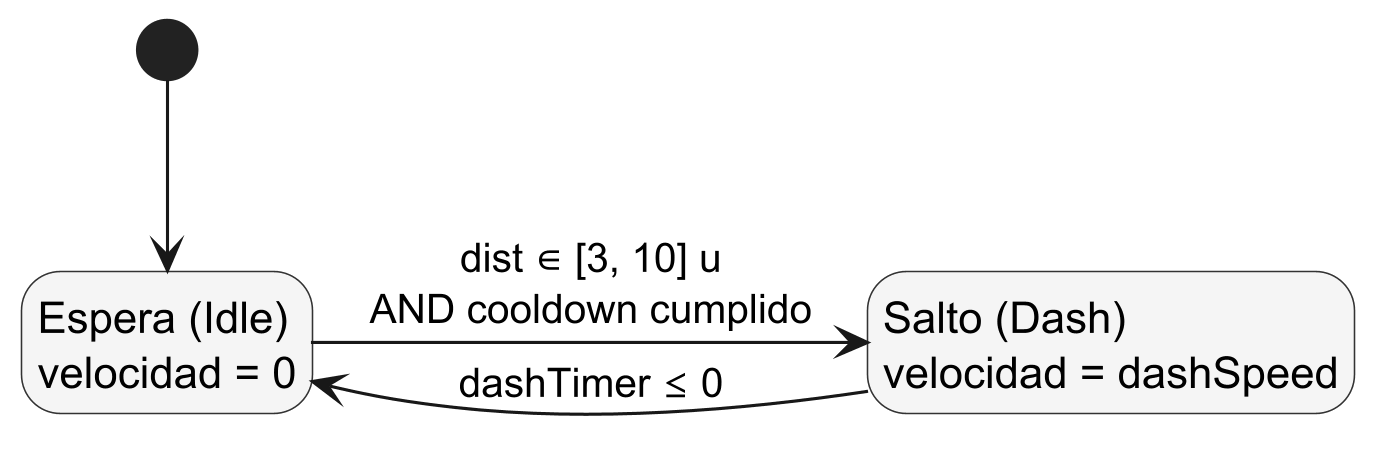
\includegraphics[width=0.95\textwidth,height=0.72\textheight,keepaspectratio]{Figuras/fsm_slimeblue.png}
\caption{
Diagrama de la FSM del SlimeBlue. \textit{Elaboración propia.}
}
\label{fig:placeholder-9}
\end{center}
\end{figure}


El método \texttt{Update()} del SlimeBlue implementa esta FSM de forma explícita, separando claramente las dos ramas de ejecución:

\begin{lstlisting}
protected override void Update() {
    base.Update();                                          // (1) Logica base heredada
    
    if (isDead || player == null) return;                   // (2) Guardas de seguridad
    
    if (!IsAIEnabled) {                                     // (3) Gracia: 0,75 s sin IA
        if (rb != null) rb.linearVelocity = Vector2.zero;
        return;
    }
    
    if (isDashing) {                                        // (4) Estado SALTO
        SetAnimatorDirection(dashDirection);                 //     Orientar animacion
        ApplyDashFacing();                                  //     Voltear todos los sprites
        dashTimer -= Time.deltaTime;                        //     Decrementar temporizador
        if (dashTimer <= 0f) {
            EndDash();                                      //     Transicion: Salto -> Espera
        }
    } else {                                                // (5) Estado ESPERA
        float distanceToPlayer = Vector2.Distance(
            transform.position, player.position);
        
        if (distanceToPlayer >= minDashDistance &&           // (6) Condicion de transicion
            distanceToPlayer <= maxDashDistance &&
            Time.time >= lastDashTime + dashCooldown) {
            StartDash();                                    //     Transicion: Espera -> Salto
        }
    }
    
    FlipSprite();                                           // (7) Orientacion visual
}
\end{lstlisting}


Línea por línea:

\begin{itemize}
\item \textbf{(1)} \texttt{base.Update()}: obligatorio para heredar la gestión de gracia y tiles de la clase base \texttt{Enemy} (patrón \textit{Template Method}).
\item \textbf{(4)} En el estado \textbf{Salto}, se actualizan la dirección del animator (\texttt{SetAnimatorDirection}) y el volteo de todos los \texttt{SpriteRenderer} del enemigo (\texttt{ApplyDashFacing}) en cada fotograma para reflejar la orientación del salto. El temporizador \texttt{dashTimer} se decrementa en cada fotograma. Cuando alcanza cero, se invoca \texttt{EndDash()}, que transita al estado \textbf{Espera} poniendo \texttt{isDashing = false}, deteniendo la velocidad y desactivando el flag de ataque del animator (\texttt{SetAnimatorAttacking(false)}).
\item \textbf{(5-6)} En el estado \textbf{Espera}, se evalúan tres condiciones conjuntas: distancia mínima (3 u), distancia máxima (10 u) y \textit{cooldown} cumplido (2 s desde el último salto). Las tres deben cumplirse simultáneamente para iniciar un nuevo salto.
\end{itemize}

La aplicación de velocidad se realiza en \texttt{FixedUpdate()}, separada de la lógica de decisión en \texttt{Update()}:

\begin{lstlisting}
private void FixedUpdate() {
    if (isDashing) {
        rb.linearVelocity = dashDirection * (dashSpeed * TileSpeedMultiplier);
    } else if (!isDead) {
        rb.linearVelocity = Vector2.zero;                   // Estatico entre saltos
    }
}
\end{lstlisting}


La separación \texttt{Update()} / \texttt{FixedUpdate()} es una decisión arquitectónica deliberada. La lógica de decisión de la FSM (¿debo saltar?) se ejecuta en \texttt{Update()} porque depende de la entrada del sistema y de temporizadores. La aplicación de velocidad al \texttt{Rigidbody2D} se ejecuta en \texttt{FixedUpdate()} porque el motor de física de Unity opera a frecuencia fija (50 Hz por defecto), y aplicar velocidad en \texttt{Update()} produciría movimiento inconsistente a distintas tasas de fotogramas.

La dirección del salto se calcula en el momento de su inicio (\texttt{StartDash()}) y permanece fija durante toda la duración del desplazamiento. Esto permite al jugador anticipar la trayectoria del salto y esquivarlo, introduciendo una componente táctica en el enfrentamiento contra este tipo de enemigo. Los parámetros del salto son: velocidad de doce unidades por segundo, duración de 0,4 segundos y tiempo de espera de dos segundos entre saltos consecutivos.

\begin{figure}[H]
\begin{center}
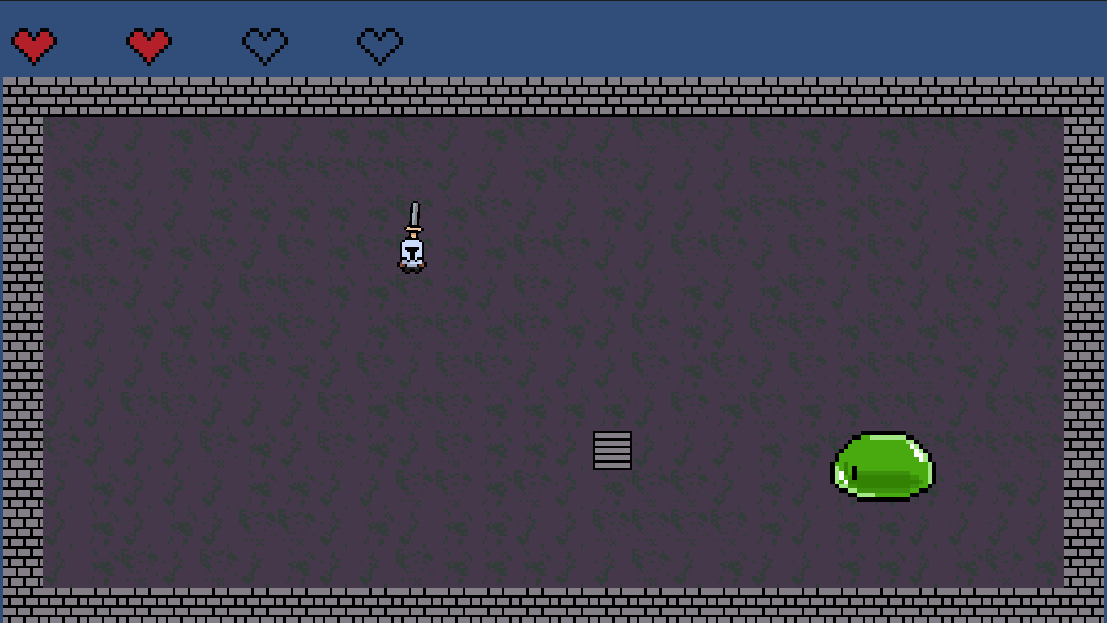
\includegraphics[width=0.9\textwidth]{Figuras/Jefe.png}
\caption{Captura de pantalla de \textit{Ascension} durante un encuentro con un enemigo jefe, mostrando el incremento visual de tamaño respecto a los enemigos estándar y los proyectiles de mayor escala. \textit{Elaboración propia.}}
\label{fig:placeholder-10}
\end{center}
\end{figure}


\textbf{Visualización durante el desarrollo.} Se implementan \textit{Gizmos} para facilitar el ajuste del rango de salto:

\begin{lstlisting}
private void OnDrawGizmosSelected() {
    Gizmos.color = Color.yellow;
    Gizmos.DrawWireSphere(transform.position, minDashDistance);
    
    Gizmos.color = Color.cyan;
    Gizmos.DrawWireSphere(transform.position, maxDashDistance);
}
\end{lstlisting}

\subsection{EnemyManager: gestión de aparición de enemigos}


El \texttt{EnemyManager} es responsable de la instanciación de enemigos en cada sala, la gestión de referencias a los enemigos activos y la detección de sala completada. Soporta dos modos de aparición:

\textbf{Modo por presupuesto de coste.} El sistema dispone de un presupuesto numérico y selecciona enemigos aleatoriamente -- ponderados por peso -- hasta agotar el presupuesto. Este mecanismo implementa una curva de dificultad \textbf{emergente}: a medida que el presupuesto crece con la profundidad de la mazmorra, el sistema puede instanciar combinaciones más peligrosas (por ejemplo, dos slimes verdes y tres rojos en lugar de solo cuatro rojos), sin necesidad de tablas de dificultad codificadas manualmente.

\begin{lstlisting}
public void SpawnByCost(Rect area, int maxCost, int depth) {
    int remaining = maxCost;                                 // (1) Presupuesto disponible
    int safety = 200;
    int spawned = 0;
    
    while (remaining >= minCost && safety-- > 0) {           // (2) Bucle de aparicion
        int totalWeight = 0;                                 // (3) Seleccion ponderada
        foreach (var a in available)
            if (a.cost <= remaining) totalWeight += a.weight;
        if (totalWeight == 0) break;
        
        int roll = Random.Range(0, totalWeight);
        GameObject chosen = null; int chosenCost = 0;
        foreach (var a in available) {
            if (a.cost > remaining) continue;
            roll -= a.weight;
            if (roll < 0) { chosen = a.prefab; chosenCost = a.cost; break; }
        }
        if (chosen == null) break;
        
        Vector2 pos = GetSafeSpawnPosition(area);            // (4) Posicion segura
        var instance = Instantiate(chosen, pos,              // (5) Instanciacion
                                   Quaternion.identity);
        
        remaining -= chosenCost;                             // (6) Decrementar presupuesto
        spawned++;
    }
}
\end{lstlisting}


Línea por línea:

\begin{itemize}
\item \textbf{(1)} \texttt{remaining} representa el presupuesto disponible para la sala actual. El presupuesto base se incrementa con \texttt{depth} (profundidad de la mazmorra), produciendo oleadas progresivamente más intensas.
\item \textbf{(2)} El bucle continúa mientras quede presupuesto suficiente para al menos el enemigo más barato (\texttt{minCost}). La variable \texttt{safety} previene bucles infinitos en caso de error de configuración (por ejemplo, si todos los costes de enemigos exceden el presupuesto restante).
\item \textbf{(3)} La selección ponderada recorre la lista de enemigos cuyo coste no exceda el presupuesto restante, acumulando sus pesos. Un valor aleatorio (\texttt{roll}) determina cuál se selecciona, de modo que enemigos con mayor peso aparecen con mayor frecuencia: un slime rojo (peso alto, coste bajo) aparece más a menudo que un slime verde (peso medio, coste alto), reflejando la intención de diseño de que el enemigo francotirador sea menos común.
\item \textbf{(4-5)} El posicionamiento seguro garantiza que ningún enemigo aparezca sobre el jugador.
\item \textbf{(6)} Decrementar el presupuesto tras instanciar produce un reparto orgánico: con presupuesto alto, el sistema puede «gastar» en enemigos caros o repartir en muchos baratos, produciendo composiciones de oleada variadas en cada sala.
\end{itemize}

\textbf{Posicionamiento seguro.} La función \texttt{GetSafeSpawnPosition} evita que los enemigos aparezcan demasiado cerca del jugador, realizando hasta 25 intentos de posicionamiento aleatorio antes de recurrir a una posición de respaldo:

\begin{lstlisting}
private Vector2 GetSafeSpawnPosition(Rect area) {
    Vector2 fallback = new Vector2(
        Random.Range(area.xMin, area.xMax),
        Random.Range(area.yMin, area.yMax));
    
    var player = GameObject.FindGameObjectWithTag("Player");
    if (player == null) return fallback;
    
    Vector2 playerPos = player.transform.position;
    float minDistSqr = safeSpawnRadius * safeSpawnRadius;
    
    for (int i = 0; i < safeSpawnAttempts; i++) {
        Vector2 candidate = new Vector2(
            Random.Range(area.xMin, area.xMax),
            Random.Range(area.yMin, area.yMax));
        if ((candidate - playerPos).sqrMagnitude >= minDistSqr)
            return candidate;
    }
    
    return fallback;
}
\end{lstlisting}


\textbf{Detección de sala completada.} En cada fotograma, el gestor elimina las referencias a enemigos destruidos y evalúa si todos los enemigos han sido eliminados. Cuando esto ocurre, emite un evento que desencadena la habilitación de las escaleras de progresión:

\begin{lstlisting}
void Update() {
    if (!roomActive) return;
    
    PruneTracked();  // Eliminar referencias nulas
    
    if (trackedEnemies.Count == 0) {
        roomActive = false;
        roomCleared = true;
        
        if (!suppressClearEvent) {
            OnRoomCleared?.Invoke();
        }
    }
}
\end{lstlisting}


\subsection{Configuración de enemigos: EnemyData}


Los datos de cada tipo de enemigo se definen mediante \textit{ScriptableObjects}. Se seleccionó este mecanismo frente a la codificación de estadísticas en los propios scripts de enemigo por la misma razón expuesta para los datos de armas: durante el desarrollo, los parámetros de equilibrado de los enemigos (vida, daño, velocidad, coste de aparición) se ajustaron iterativamente más de diez veces, y cada ajuste con \textit{ScriptableObjects} es inmediato y no requiere recompilación.

\begin{lstlisting}
[CreateAssetMenu(menuName = "Enemies/EnemyData")]
public class EnemyData : ScriptableObject {
    public string enemyName;      // Identificador visible ("Slime Verde")
    public int maxHealth = 3;     // Puntos de vida maximos
    public int damage = 1;        // Dano infligido por contacto o proyectil
    public float speed = 2f;      // Velocidad base en unidades/segundo
    public Sprite sprite;         // Sprite principal del enemigo
    public int enemyCost;         // Coste de aparicion en el sistema de presupuesto
}
\end{lstlisting}


El campo \texttt{enemyCost} merece una explicación específica: define cuánto "cuesta" instanciar este enemigo dentro del sistema de presupuesto del \texttt{EnemyManager}. Un slime rojo (perseguidor, fácil de esquivar) tiene un coste bajo, mientras que un slime verde (francotirador, más peligroso) tiene un coste superior. El presupuesto total del \texttt{EnemyManager} se incrementa con la profundidad de la mazmorra, produciendo oleadas progresivamente más intensas sin necesidad de tablas de dificultad codificadas manualmente. Esta decisión reduce el acoplamiento entre el sistema de dificultad y los tipos de enemigo: añadir un nuevo tipo de enemigo con su \texttt{enemyCost} correspondiente integra automáticamente ese enemigo en la curva de dificultad sin modificar el código del \texttt{EnemyManager}.

\subsection{Síntesis comparativa de los tipos de enemigo}


La siguiente tabla resume las diferencias de comportamiento, parámetros y rol táctico entre los tres tipos de enemigo, mostrando cómo la jerarquía basada en el patrón \textit{Template Method} permite diferenciar la IA sin duplicar la lógica base compartida:

\begin{table}[H]
\begin{center}
\small
\begin{tabular}{|p{0.23\textwidth}|p{0.23\textwidth}|p{0.23\textwidth}|p{0.23\textwidth}|}
\hline
\textbf{Aspecto} & \textbf{SlimeRed (perseguidor)} & \textbf{SlimeGreen (francotirador)} & \textbf{SlimeBlue (saltador)} \\ \hline
Comportamiento de IA & Persecución directa constante & FSM de 3 estados (huir, acercarse, disparar) & Ciclo de espera y salto (\textit{dash}) \\ \hline
Método principal sobrescrito & \texttt{Update()} -> \texttt{ChasePlayer()} & \texttt{Update()} -> \texttt{Escape()} / \texttt{Approach()} / \texttt{Shoot()} & \texttt{Update()} -> \texttt{StartDash()} / \texttt{EndDash()} \\ \hline
Movimiento & \texttt{rb.linearVelocity} hacia el jugador & \texttt{rb.linearVelocity} según zona de distancia & \texttt{rb.linearVelocity} solo durante el salto \\ \hline
Distancia al jugador & Siempre se acerca (0 m ideales) & Mantiene distancia óptima (4–12 unidades) & Rango de activación (3–10 unidades) \\ \hline
Mecánica de daño & Contacto directo & Proyectil a distancia (\texttt{EnemyProjectile}) & Contacto durante el salto \\ \hline
Velocidad base & \texttt{moveSpeed} $\times$ \texttt{TileSpeedMultiplier} & Limitada por \texttt{CapToPlayerSpeed} & \texttt{dashSpeed} = 12 u/s durante 0,4 s \\ \hline
Tiempo de espera & Ninguno (acción continua) & \texttt{shootCooldown} entre disparos & \texttt{dashCooldown} = 2 s entre saltos \\ \hline
Coste de aparición & Bajo (fácil de esquivar) & Alto (peligroso a distancia) & Medio (predecible pero rápido) \\ \hline
Rol táctico & Presión constante, obliga a moverse & Obliga a cerrar distancia o usar arma a distancia & Requiere anticipación y esquiva \\ \hline
Contramedida del jugador & Arma cuerpo a cuerpo y kiting & Arma a distancia o persecución rápida & Esquiva (\textit{roll}) y posicionamiento \\ \hline
\end{tabular}
\end{center}
\end{table}


\TablaTitulo{Comparativa de comportamiento, parámetros y rol táctico de los tres tipos de enemigo.
}

La diversidad de estos tres arquetipos, combinada con el sistema de presupuesto de coste del \texttt{EnemyManager} y la variabilidad de los tiles especiales, produce situaciones de combate tácticas y diferenciadas en cada sala sin necesidad de un repertorio extenso de tipos de enemigo.

\subsection{Diagrama de flujo de decisión de la IA por tipo de enemigo}


El siguiente diagrama de flujo unificado muestra la lógica de decisión completa que ejecuta cada tipo de enemigo en cada fotograma, incluyendo la lógica heredada de la clase base \texttt{Enemy} (común a los tres) y la lógica específica de cada subclase:

\begin{figure}[H]
\begin{center}
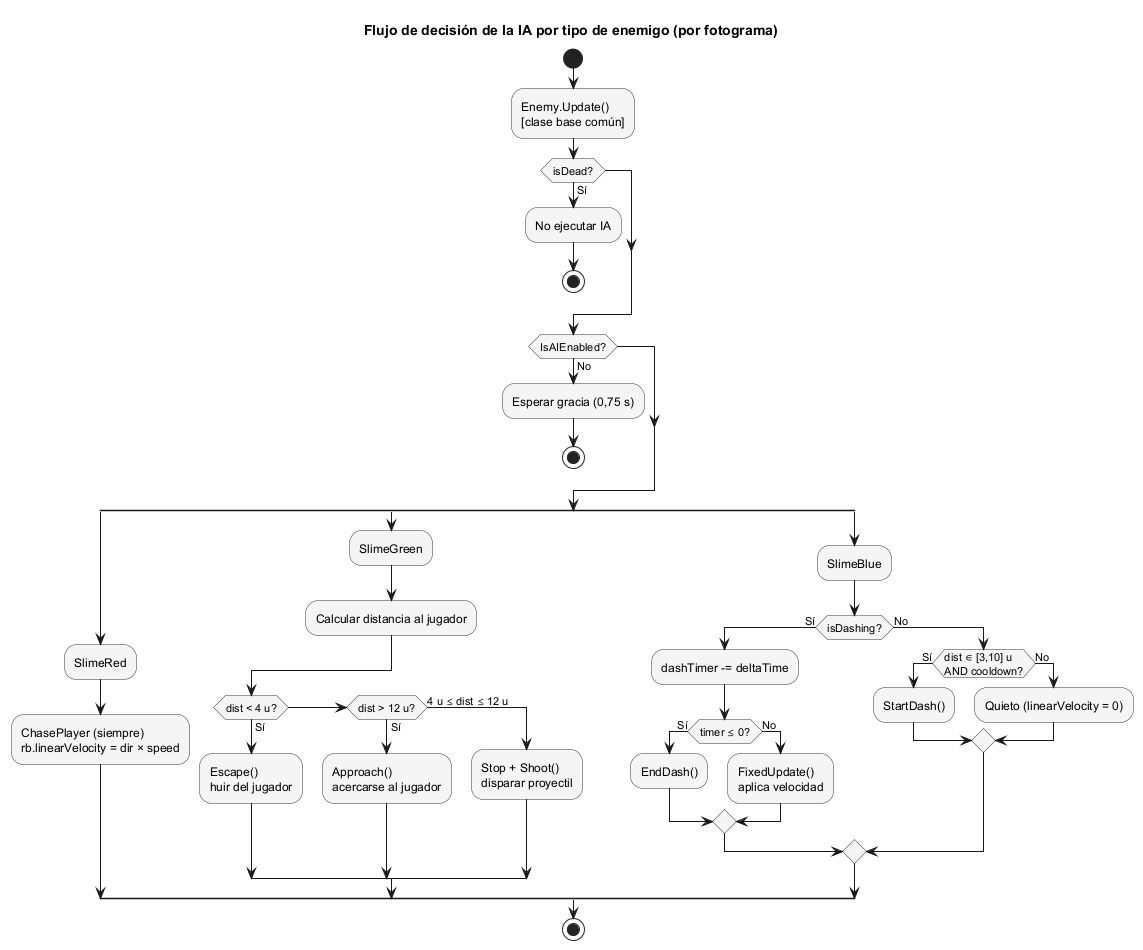
\includegraphics[width=0.95\textwidth,height=0.72\textheight,keepaspectratio]{Figuras/flujo_decision_ia.png}
\caption{
Diagrama de flujo de decisión de la IA por tipo de enemigo. \textit{Elaboración propia.}
}
\label{fig:placeholder-12}
\end{center}
\end{figure}


Este diagrama evidencia una propiedad del diseño: la lógica heredada de la clase base \texttt{Enemy} (verificaciones de muerte, gracia y tiles) se ejecuta siempre \textit{antes} que la lógica específica de cada subclase, garantizando que las comprobaciones de seguridad son comunes e inmutables --un ejemplo concreto del contrato impuesto por el patrón \textit{Template Method}.

\begin{figure}[H]
\begin{center}
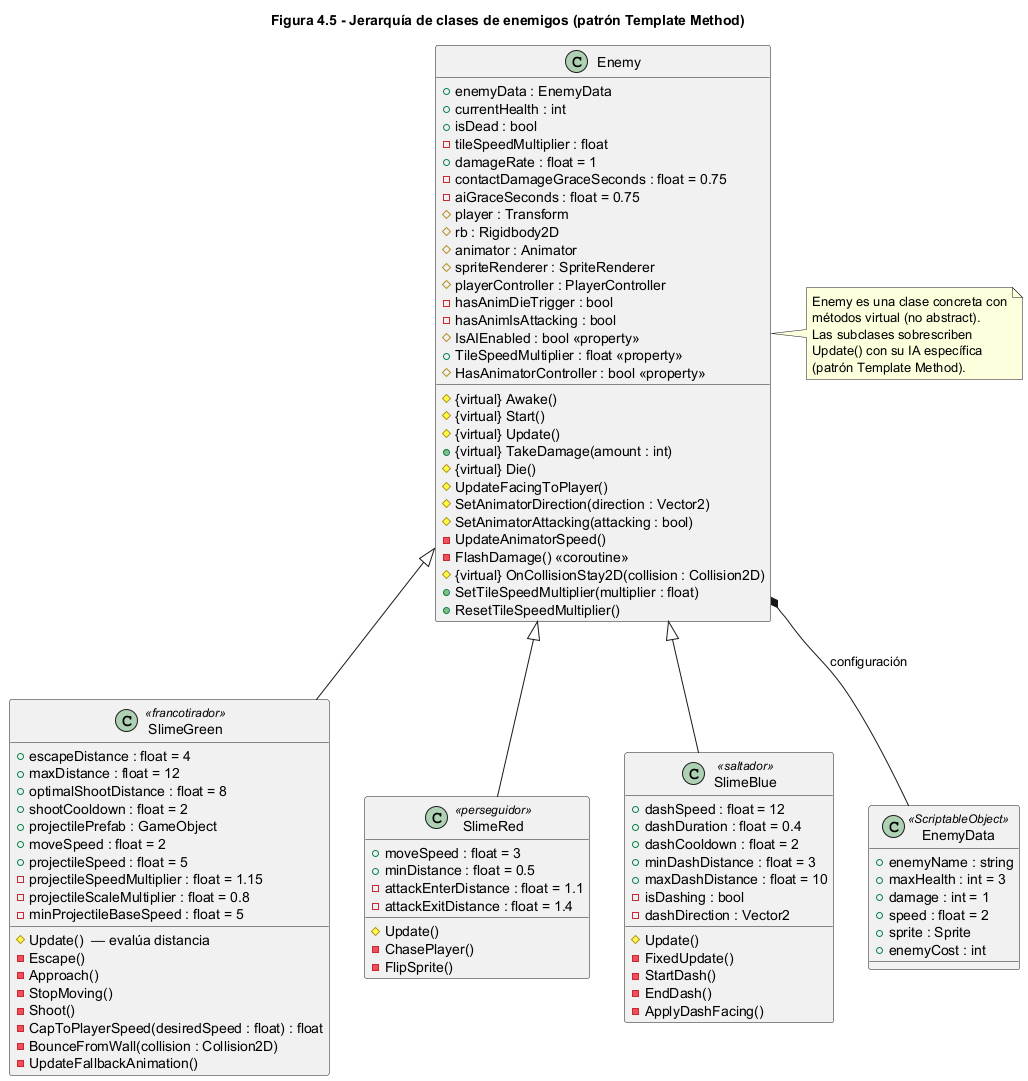
\includegraphics[width=0.95\textwidth,height=0.72\textheight,keepaspectratio]{Figuras/figura4_5_clases_enemigos.png}
\caption{
Diagrama de clases UML de la jerarquía de enemigos. \textit{Elaboración propia.}
}
\label{fig:placeholder-13}
\end{center}
\end{figure}


\begin{figure}[H]
\begin{center}
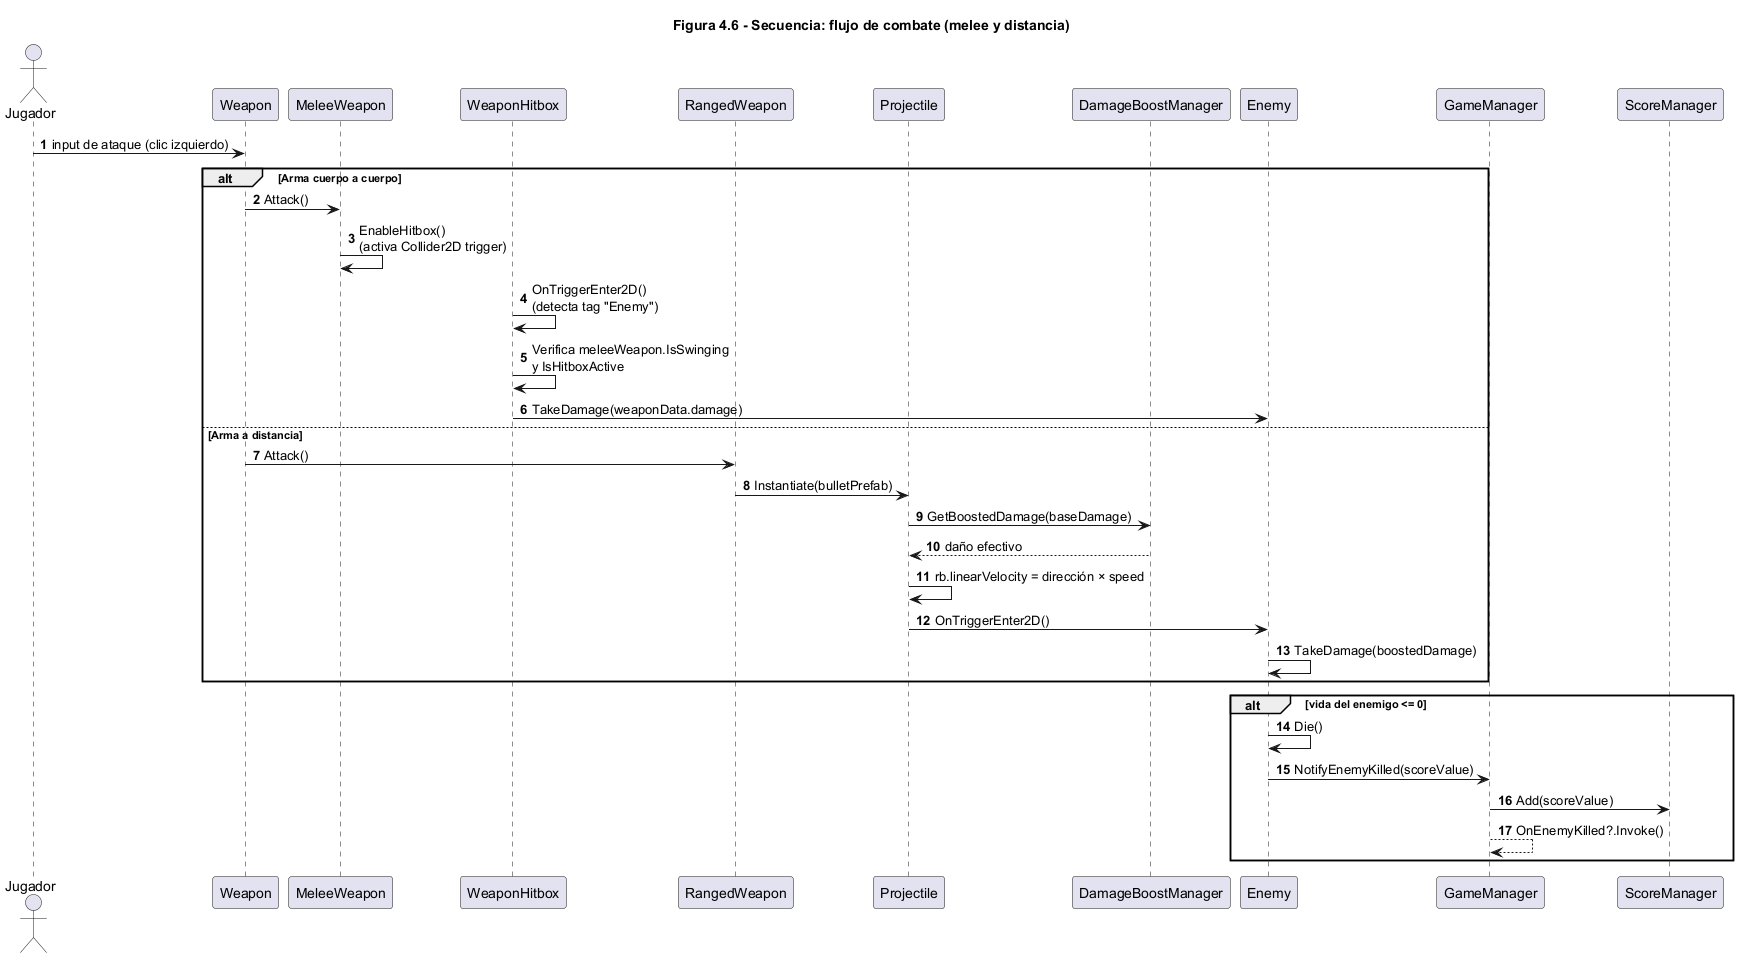
\includegraphics[width=0.95\textwidth,height=0.72\textheight,keepaspectratio]{Figuras/figura4_6_secuencia_combate.png}
\caption{
Diagrama de secuencia UML del flujo de combate. \textit{Elaboración propia.}
}
\label{fig:placeholder-14}
\end{center}
\end{figure}


\section{Sistema de armas y combate}


\textbf{Evolución iterativa.} El sistema de armas pasó por dos rediseños. La primera versión implementaba una clase única \texttt{Weapon} con un enumerado \texttt{WeaponType} y bloques condicionales que diferenciaban el comportamiento cuerpo a cuerpo del comportamiento a distancia; esta estructura se volvió difícil de mantener al añadir los efectos visuales (\textit{weapon trail}, parpadeo de hitbox), ya que cada tipo de arma requería campos y lógica distintos dentro de la misma clase. La refactorización al patrón \textit{Strategy} -- con \texttt{Weapon} como clase base y \texttt{MeleeWeapon} / \texttt{RangedWeapon} como estrategias concretas -- resolvió este problema. La animación de barrido del arma cuerpo a cuerpo se rediseñó de interpolación lineal a sinusoidal tras observar que el movimiento uniforme transmitía una sensación mecánica carente del «peso» visual esperado en un arma.

\subsection{Weapon: clase base del sistema de armas y patrón \textit{Strategy}}


El sistema de armas implementa el patrón \textit{Strategy}. Se seleccionó este patrón frente a la alternativa de una única clase \texttt{Weapon} con un enumerado \texttt{WeaponType} y bloques condicionales (\texttt{if (type == Melee) ... else if (type == Ranged) ...}). Esta alternativa se descartó por dos razones: en primer lugar, cada tipo de arma requiere campos específicos distintos -- \texttt{swingAngle} y \texttt{swingDuration} para las armas cuerpo a cuerpo, \texttt{bulletPrefab} y \texttt{attackCooldown} para las armas a distancia --, lo que produciría una clase con campos que solo son relevantes para uno de los tipos; en segundo lugar, añadir un tercer tipo de arma obligaría a modificar la lógica interna de la clase existente, violando el principio de apertura-cierre.

El patrón \textit{Strategy} resuelve ambos problemas: la clase base \texttt{Weapon} define la interfaz común (\texttt{Attack()}, rotación hacia el cursor, órbita alrededor del jugador) y las subclases \texttt{MeleeWeapon} y \texttt{RangedWeapon} encapsulan únicamente los campos y la lógica relevantes para su tipo de ataque.

\textbf{Sistema de rotación y órbita.} El arma sigue la posición del cursor del ratón y orbita alrededor del jugador:

\begin{lstlisting}
private void RotateTowardsMouse() {
    Vector3 mouseWorldPosition = camera.ScreenToWorldPoint(Input.mousePosition);
    mouseWorldPosition.z = 0;
    
    Vector2 direction = (mouseWorldPosition - transform.position).normalized;
    float angle = Mathf.Atan2(direction.y, direction.x) * Mathf.Rad2Deg;
    
    float spriteOrientationOffset = -90f;
    transform.rotation = Quaternion.Euler(0, 0, angle + spriteOrientationOffset);
}
\end{lstlisting}


La conversión de la posición del ratón de coordenadas de pantalla a coordenadas del mundo se realiza mediante \texttt{Camera.ScreenToWorldPoint}. El ángulo de rotación se calcula mediante \texttt{Mathf.Atan2(direction.y, direction.x)}, que retorna el ángulo en radianes del vector dirección respecto al eje X positivo; la multiplicación por \texttt{Mathf.Rad2Deg} convierte a grados para aplicarlo como rotación del \texttt{transform}. El desplazamiento de -90º (\texttt{spriteOrientationOffset}) compensa que los sprites de las armas están orientados hacia arriba en su fichero de origen: sin este ajuste, un ángulo de 0º apuntaría el sprite hacia la derecha en lugar de hacia arriba.

Se seleccionó el cálculo trigonométrico (\texttt{Atan2} + rotación Euler) frente a la alternativa de usar \texttt{Quaternion.LookRotation}, porque esta última está orientada al espacio 3D y requiere una conversión adicional para obtener una rotación exclusivamente en el eje Z, lo que introduce complejidad innecesaria en un proyecto 2D.

\subsection{MeleeWeapon: armas cuerpo a cuerpo}


El \texttt{MeleeWeapon} implementa un ataque de barrido (\textit{swing}) con un arco configurable de 180 grados y una animación procedural:

\begin{lstlisting}
protected override void Update() {
    base.Update();
    
    // Cancelar swing si el jugador suelta el boton del raton a mitad de ataque
    if (!Input.GetMouseButton(0) && isSwinging) {
        StopSwinging();
        return;
    }
    
    if (isSwinging) {
        swingTimer += Time.deltaTime;
        float progress = swingTimer / swingDuration;
        
        if (progress >= 1f) {
            StopSwinging();
        } else {
            float smoothProgress = Mathf.Sin(progress * Mathf.PI);
            float currentSwingOffset = Mathf.Lerp(
                -swingAngle / 2, 
                swingAngle / 2, 
                smoothProgress
            );
            
            Vector3 currentRotation = transform.localEulerAngles;
            currentRotation.z = swingStartAngle + currentSwingOffset;
            transform.localRotation = Quaternion.Euler(currentRotation);
        }
    }
}
\end{lstlisting}


La animación del barrido utiliza una curva sinusoidal (\texttt{Mathf.Sin}) para producir un movimiento suave que acelera al inicio y desacelera al final, resultando en una sensación de peso y naturalidad. Se seleccionó la interpolación sinusoidal frente a una interpolación lineal (\texttt{Mathf.Lerp} con progreso lineal) porque esta última produce un movimiento uniforme que transmite una sensación mecánica, carente del «peso» visual que se espera de un arma cuerpo a cuerpo. Si el jugador suelta el botón del ratón durante el barrido, este se cancela inmediatamente mediante \texttt{StopSwinging()}, que centraliza la desactivación de la hitbox y el rastro visual (\texttt{WeaponTrail}) en un único método, evitando la duplicación de lógica de limpieza.

Línea por línea del fragmento:

\begin{itemize}
\item \texttt{swingTimer += Time.deltaTime}: acumula el tiempo transcurrido desde el inicio del barrido, independientemente de la tasa de fotogramas.
\item \texttt{float progress = swingTimer / swingDuration}: normaliza el progreso del barrido al rango [0, 1], donde 0 es el inicio y 1 es el final.
\item \texttt{Mathf.Sin(progress * Mathf.PI)}: convierte el progreso lineal en una curva sinusoidal. Cuando \texttt{progress = 0}, el seno vale 0; cuando \texttt{progress = 0.5}, vale 1 (máximo desplazamiento); cuando \texttt{progress = 1}, vuelve a 0.
\item \texttt{Mathf.Lerp(-swingAngle/2, swingAngle/2, smoothProgress)}: mapea el progreso sinusoidal a un ángulo de rotación dentro del rango [-90º, +90º], produciendo el arco de 180º configurable.
\item \texttt{StopSwinging()}: al completar el barrido (\texttt{progress >= 1}) o al soltar el botón, desactiva la hitbox, detiene el rastro visual y marca \texttt{isSwinging = false}.
\end{itemize}

\textbf{Detección de impacto.} Durante el barrido, la hitbox del arma detecta colisiones con enemigos. Si existen componentes \texttt{WeaponHitbox} hijos, la detección se delega a ellos para evitar daño duplicado; en caso contrario, el propio \texttt{MeleeWeapon} verifica las condiciones de activación:

\begin{lstlisting}
private void OnTriggerEnter2D(Collider2D other) {
    // Si hay WeaponHitbox hijos, ellos gestionan el dano
    if (weaponHitboxes != null && weaponHitboxes.Length > 0) return;
    if (!isSwinging || !hitboxesActive) return;
    if (hitbox == null || !hitbox.enabled) return;
    
    if (other.CompareTag("Enemy") && weaponData != null) {
        Enemy enemy = other.GetComponent<Enemy>();
        if (enemy != null)
            enemy.TakeDamage(weaponData.damage);
    }
}
\end{lstlisting}


\subsection{RangedWeapon: armas a distancia}


El \texttt{RangedWeapon} implementa el ataque mediante la instanciación de proyectiles:

\begin{lstlisting}
public override void Attack() {
    if (Time.time < lastAttackTime + attackCooldown) return;
    
    if (weaponData?.bulletPrefab != null) {
        lastAttackTime = Time.time;
        
        Vector3 spawnPosition = spawner?.position ?? transform.position;
        Quaternion spawnRotation = transform.rotation;
        
        GameObject bullet = Instantiate(
            weaponData.bulletPrefab, 
            spawnPosition, 
            spawnRotation
        );
        
        Projectile projectileScript = bullet.GetComponent<Projectile>();
        if (projectileScript != null) {
            projectileScript.damage = weaponData.damage;
            projectileScript.speed = 10f;
        }
    }
}
\end{lstlisting}


El operador \texttt{?.} (operador condicional nulo) evita excepciones cuando una referencia es nula. El operador \texttt{??} (operador de coalescencia nula) proporciona un valor de respaldo cuando el valor principal es nulo.

\subsection{Projectile: comportamiento de proyectiles}


El componente \texttt{Projectile} controla el movimiento lineal del proyectil, su autodestrucción por tiempo de vida y la integración con el sistema de bonificación de daño:

\begin{lstlisting}
void Start() {
    if (DamageBoostManager.Instance != null) {
        damage = DamageBoostManager.Instance.GetBoostedDamage(damage);
    }
    
    if (rb != null) {
        rb.linearVelocity = transform.up * speed;
    }
    
    Destroy(gameObject, lifetime);
}
\end{lstlisting}


La consulta al \texttt{DamageBoostManager} permite que los proyectiles se beneficien de las bonificaciones de daño otorgadas por los tiles de potenciación. La llamada a \texttt{Destroy(gameObject, lifetime)} programa la destrucción automática del proyectil tras un tiempo configurable, evitando la acumulación de objetos fuera de los límites de la sala.

\textbf{Detección de impacto.} Al colisionar, el proyectil aplica daño a los enemigos y se destruye al contactar con paredes o enemigos. Los proyectiles del jugador ignoran explícitamente las armas del propio jugador para evitar colisiones involuntarias:

\begin{lstlisting}
void OnTriggerEnter2D(Collider2D other) {
    if (other.CompareTag("Player") || other.CompareTag("Weapon")
        || other.GetComponent<Weapon>() != null)
        return;
    
    if (other.CompareTag("Enemy")) {
        Enemy enemy = other.GetComponent<Enemy>();
        if (enemy != null)
            enemy.TakeDamage(damage);
    }
    
    if (other.CompareTag("Wall") || other.CompareTag("Enemy"))
        Destroy(gameObject);
}
\end{lstlisting}


La comprobación combinada de la etiqueta \texttt{"Weapon"} y del componente \texttt{Weapon} proporciona una doble verificación: la etiqueta cubre los casos estándar, mientras que la comprobación de componente cubre prefabs que pudieran no tener la etiqueta asignada.

\subsection{WeaponData: configuración de armas mediante \textit{ScriptableObjects}}


Los datos de cada arma se definen mediante \textit{ScriptableObjects}, manteniendo la separación entre datos y lógica. Al igual que con \texttt{PlayerClass} y \texttt{EnemyData}, se seleccionó este mecanismo frente a la codificación directa de parámetros en los scripts de arma. Esta decisión permite que el mismo prefab de \texttt{MeleeWeapon} se reutilice con distintas configuraciones (espada, hacha, lanza) simplemente asignando un \textit{ScriptableObject} diferente, sin duplicar prefabs ni código:

\begin{lstlisting}
[CreateAssetMenu(menuName = "Items/WeaponData")]
public class WeaponData : ScriptableObject {
    public string weaponName;         // Nombre visible del arma
    public int damage;                // Dano base por impacto
    public float atackSpeed;          // Velocidad de ataque (tiempo de espera entre ataques)
    public Sprite sprite;             // Sprite visual del arma
    public GameObject bulletPrefab;   // Prefab del proyectil (solo para armas a distancia; null para melee)
    public GameObject weaponPrefab;   // Prefab del GameObject completo del arma
}
\end{lstlisting}


Línea por línea:

\begin{itemize}
\item \texttt{damage}: daño base que puede ser modificado en tiempo de ejecución por el \texttt{DamageBoostManager} cuando el jugador se encuentra sobre un tile de potenciación.
\item \texttt{bulletPrefab}: referencia condicional -- solo las armas a distancia la utilizan; las armas cuerpo a cuerpo la dejan como \texttt{null}. El código de \texttt{RangedWeapon.Attack()} verifica esta referencia antes de instanciar proyectiles mediante el operador condicional nulo (\texttt{?.}).
\item \texttt{weaponPrefab}: referencia al prefab preconfigurado que incluye el componente \texttt{MeleeWeapon} o \texttt{RangedWeapon}, los colisionadores, el \textit{SpriteRenderer} y los efectos visuales.
\end{itemize}

\subsection{Flujo completo de daño: del ataque a la puntuación}


El sistema de combate involucra a cinco componentes distribuidos en tres subsistemas (armas, enemigos y gestión central). El siguiente diagrama describe la cadena completa de invocaciones que se produce cuando el jugador ataca a un enemigo, desde la entrada del jugador hasta la actualización de la puntuación:
\vspace{-0.5em}
\begin{figure}[H]
\begin{center}
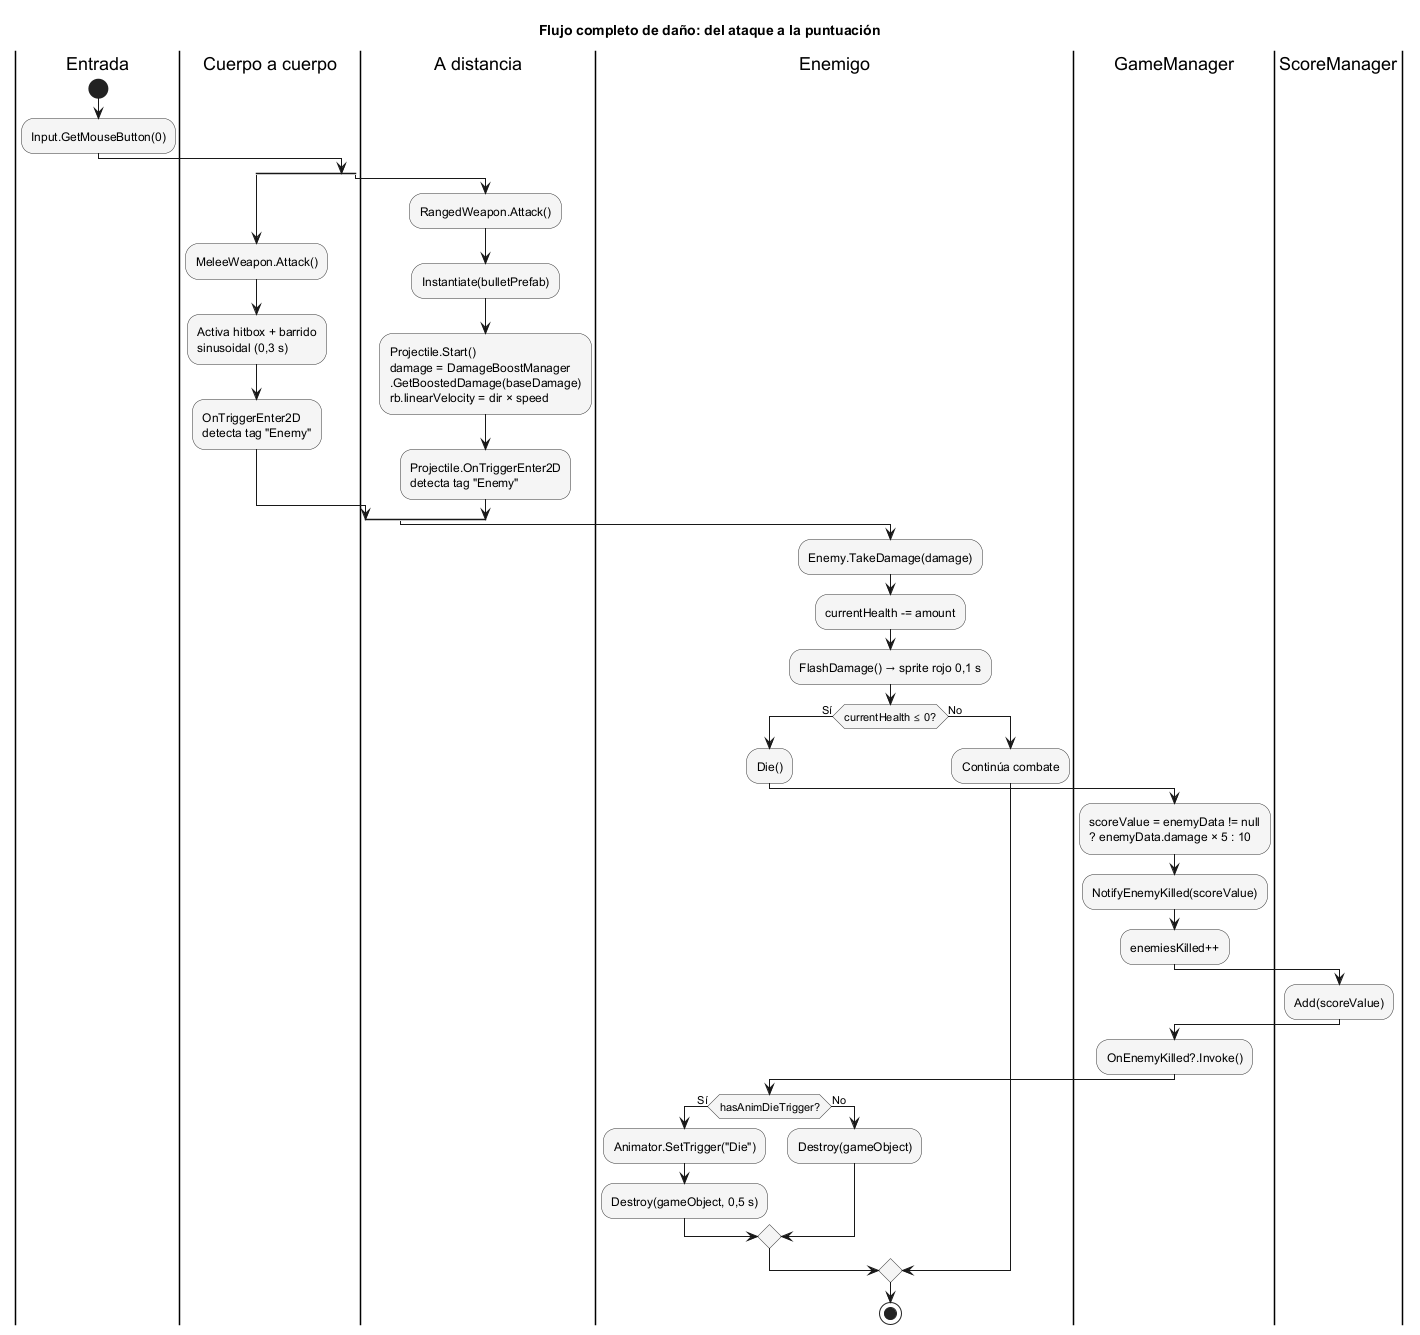
\includegraphics[width=0.95\textwidth,height=0.72\textheight,keepaspectratio]{Figuras/flujo_dano_completo.png}
\caption{
Diagrama de flujo del sistema de daño. \textit{Elaboración propia.}
}
\label{fig:placeholder-16}
\end{center}
\end{figure}
\vspace{-0.5em}

Este flujo evidencia la separación de responsabilidades aplicada: cada componente ejecuta exclusivamente su tarea (el arma ataca, el enemigo recibe daño, el gestor contabiliza) y la comunicación entre capas se realiza mediante invocaciones directas tipadas y eventos del patrón \textit{Observer}. La alternativa -- que el arma calculase ella misma la puntuación, o que el enemigo accediese directamente al marcador de la UI -- habría introducido dependencias transversales entre subsistemas que no comparten responsabilidad.
\vspace{-0.5em}
\begin{figure}[H]
\begin{center}
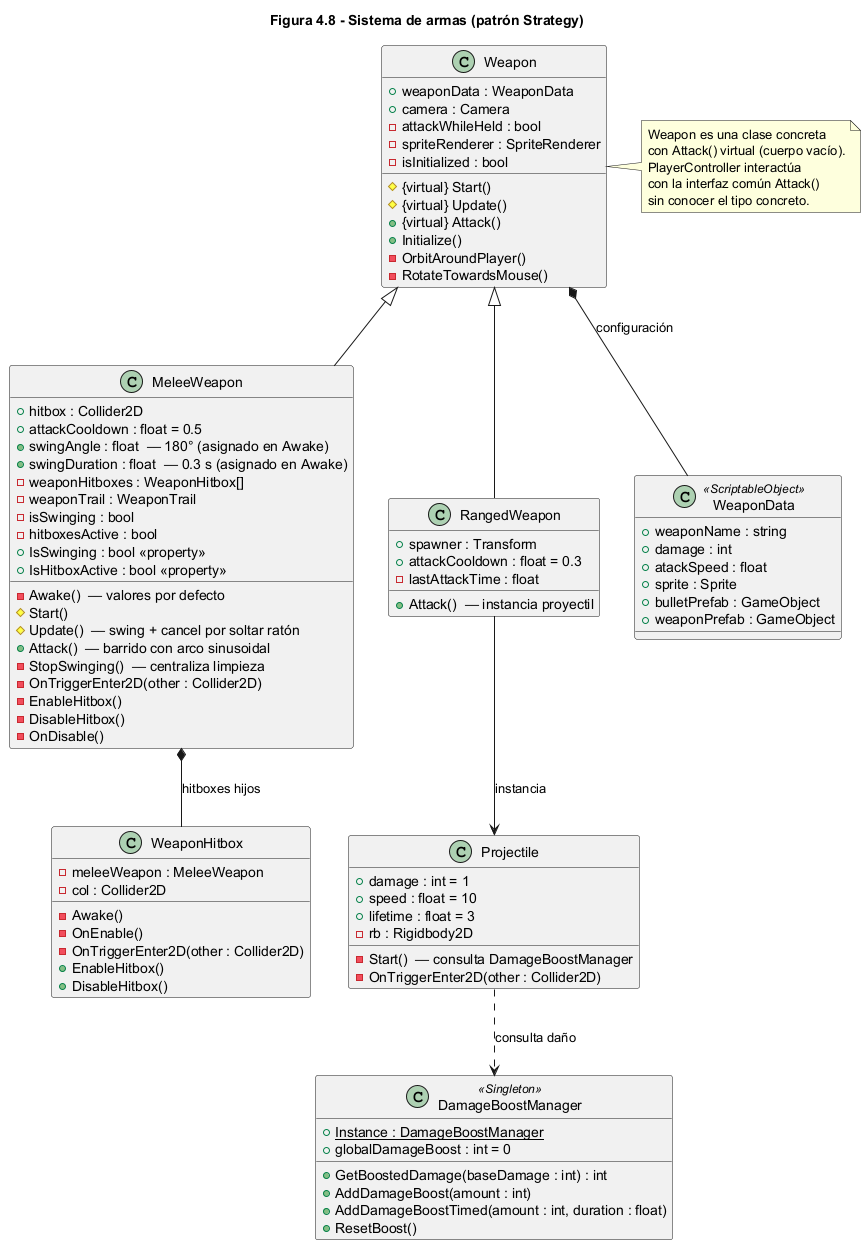
\includegraphics[width=0.95\textwidth,height=0.72\textheight,keepaspectratio]{Figuras/figura4_8_clases_armas.png}
\caption{
Diagrama de clases UML del sistema de armas. \textit{Elaboración propia.}
}
\label{fig:placeholder-17}
\end{center}
\end{figure}


\section{Sistema de generación procedural}


\textbf{Evolución iterativa.} La generación procedural fue el subsistema con mayor impacto arquitectónico derivado de la iteración. El diseño inicial cargaba una nueva escena de Unity para cada sala, lo que provocaba tiempos de carga de 0,5 a 1,5 segundos que rompían el ritmo de juego. El rediseño hacia la regeneración del \textit{tilemap} dentro de la misma escena (\texttt{RegenerateFloorKeepWalls}) eliminó estos tiempos de carga y modificó las responsabilidades del \texttt{RoomFlowController}. Adicionalmente, la distribución de tiles especiales evolucionó de una colocación puramente aleatoria (tile a tile) a un sistema de \textit{clusters} por expansión radial: la distribución aleatoria producía tiles aislados cuyo efecto era imperceptible durante el juego, mientras que los \textit{clusters} de 4-9 tiles generan zonas tácticas significativas que el jugador puede utilizar o evitar de forma deliberada.

\subsection{RoomGenerator: generación de salas}


El \texttt{RoomGenerator} constituye uno de los componentes de mayor complejidad del proyecto. Es responsable de la generación procedural de las salas del juego, incluyendo la estructura de muros, la distribución de tiles de suelo con variantes visuales y la colocación de tiles especiales con efectos.

Se seleccionó un enfoque de rejilla rectangular fija frente a alternativas más sofisticadas como BSP (\textit{Binary Space Partitioning}) o WFC (\textit{Wave Function Collapse}) por tres razones que afectan directamente a la jugabilidad y la complejidad de implementación:

\begin{enumerate}
\item \textbf{Simplicidad de posicionamiento de enemigos.} Con una rejilla rectangular fija de límites conocidos, cualquier coordenada dentro del perímetro de muros constituye una posición válida para la aparición de enemigos. Con BSP, las salas tendrían formas irregulares conectadas por pasillos estrechos, lo que requeriría verificaciones adicionales de accesibilidad y de línea de visión entre el jugador y el punto de aparición.
\item \textbf{Contención automática.} Los bordes perimetrales de muros generan colisionadores automáticos mediante el \texttt{TilemapCollider2D}, impidiendo que el jugador abandone el área de juego sin lógica de contención adicional.
\item \textbf{Variabilidad táctica mediante tiles.} La variabilidad entre salas no reside en la forma geométrica del espacio, sino en la distribución de tiles especiales dentro de él. Este enfoque combina la previsibilidad estructural (el jugador siempre sabe el tamaño de la sala) con la imprevisibilidad táctica (la ubicación de zonas de hielo, lodo y potenciación cambia en cada sala).
\end{enumerate}

\textbf{Configuración de la sala.} Cada sala se genera sobre una rejilla de $26 \times 12$ tiles, con un borde perimetral de muros de 1 tile de grosor:

\begin{lstlisting}
[SerializeField] private int roomWidth = 26;
[SerializeField] private int roomHeight = 12;
[SerializeField] private int wallBorderThicknessTiles = 1;
\end{lstlisting}


\textbf{Algoritmo de generación.} El proceso de generación de una sala sigue una secuencia de cinco pasos. A continuación se muestra la estructura real del método \texttt{GenerateRoom()} de \texttt{RoomGenerator.cs}, simplificada para mayor claridad:

\begin{lstlisting}
public void GenerateRoom() {
    // 1. Limpiar tilemaps anteriores
    if (clearWalls) wallTilemap.ClearAllTiles();
    floorTilemap.ClearAllTiles();

    // 2. Rellenar suelo y colocar tiles especiales en clusters
    for (int x = 0; x < roomWidth; x++)
        for (int y = 0; y < roomHeight; y++)
            floorTilemap.SetTile(pos, GetRandomNormalFloorTile());
    PlaceSpecialTilesClustered();   // hielo, lodo, curacion, potenciacion

    // 3. Colocar escaleras (en cada sala, en posicion aleatoria con margen)
    PlaceStairsTile();

    // 4. Generar borde de muros perimetrales (bucles inline)
    // wallTilemap.SetTile(...) en cada posicion del perimetro

    // 5. Actualizar colisionadores
    RefreshWallColliders();
    EnsureBoundaryCollidersSetup();
}
\end{lstlisting}


\textbf{Paso 1: Limpieza.} Se eliminan todos los tiles existentes en ambos \textit{tilemaps} (muros y suelo) mediante \texttt{wallTilemap.ClearAllTiles()} y \texttt{floorTilemap.ClearAllTiles()}, preparando la rejilla para una nueva generación.

\textbf{Paso 2: Generación de suelo con clusters.} Este paso constituye el núcleo del algoritmo de generación procedural. Primero se rellena toda la superficie interior con tiles normales seleccionados aleatoriamente entre las variantes disponibles. A continuación, se aplica el algoritmo de expansión por \textit{clusters} para colocar los tiles especiales.

\textbf{Algoritmo de expansión por \textit{clusters}.} Los tiles de hielo y lodo se distribuyen en manchas orgánicas de entre 4 y 9 tiles, generadas mediante un algoritmo de expansión por adyacencia de 4 direcciones desde un centro aleatorio. El método \texttt{PaintCluster} implementa esta lógica:

\begin{lstlisting}
private void PaintCluster(Vector2Int center, int targetCount, int maxRadius,
                          TileBase tile, HashSet<Vector2Int> reserved, int padding) {
    int minX = padding;
    int maxX = roomWidth - 1 - padding;
    int minY = padding;
    int maxY = roomHeight - 1 - padding;
    
    bool InBounds(Vector2Int c) =>
        c.x >= minX && c.x <= maxX && c.y >= minY && c.y <= maxY;
    int Manhattan(Vector2Int a, Vector2Int b) =>
        Mathf.Abs(a.x - b.x) + Mathf.Abs(a.y - b.y);
    
    var painted = new List<Vector2Int>(targetCount);
    if (InBounds(center) && reserved.Add(center)) {
        painted.Add(center);
        floorTilemap.SetTile(new Vector3Int(center.x, center.y, 0) + roomOffset, tile);
    }
    
    Vector2Int[] dirs = { Vector2Int.right, Vector2Int.left,
                          Vector2Int.up, Vector2Int.down };
    int safety = 200;
    while (painted.Count < targetCount && safety-- > 0) {
        if (painted.Count == 0) break;
        var baseCell = painted[Random.Range(0, painted.Count)];
        var next = baseCell + dirs[Random.Range(0, dirs.Length)];
        
        if (!InBounds(next)) continue;
        if (Manhattan(next, center) > maxRadius) continue;
        if (!reserved.Add(next)) continue;
        
        painted.Add(next);
        floorTilemap.SetTile(new Vector3Int(next.x, next.y, 0) + roomOffset, tile);
    }
}
\end{lstlisting}


El algoritmo comienza seleccionando una posición aleatoria como centro del \textit{cluster}. A continuación, expande el \textit{cluster} seleccionando en cada iteración una celda pintada al azar y desplazándose en una de las cuatro direcciones cardinales. La función local \texttt{InBounds} verifica que la posición candidata se encuentra dentro del margen útil del suelo (excluyendo un borde de \texttt{padding} celdas), y el \texttt{HashSet<Vector2Int> reserved} impide que una misma celda se pinte dos veces o sea reclamada por \textit{clusters} diferentes. La restricción de distancia Manhattan respecto al centro garantiza que el \textit{cluster} no se extienda más allá del radio máximo, produciendo manchas compactas de forma irregular y orgánica.


Este \textit{pipeline} se ejecuta también -- con una variante -- cuando el jugador avanza a la siguiente sala dentro de la misma escena: \texttt{RegenerateFloorKeepWalls()} omite los pasos 4 y 5 (los muros perimetrales no cambian) y únicamente regenera el suelo, los tiles especiales y las escaleras, reduciendo el coste computacional de la transición.

\textbf{Probabilidades de aparición de tiles especiales:}
\vspace{-0.5em}
\begin{table}[H]
\begin{center}
\small
\begin{tabular}{|p{0.22\textwidth}|p{0.18\textwidth}|p{0.25\textwidth}|p{0.18\textwidth}|}
\hline
\textbf{Tipo de tile} & \textbf{Probabilidad} & \textbf{Formato} & \textbf{Cantidad por sala} \\ \hline
Curación (\textit{Heal}) & 2 \% & Tile individual & Máximo 1 \\ \hline
Hielo (\textit{Ice}) & 12 \% & Cluster de 4-9 tiles & Variable \\ \hline
Lodo (\textit{Mud}) & 12 \% & Cluster de 4-9 tiles & Variable \\ \hline
Potenciación (\textit{PowerUp}) & 18 \% & Tile individual & 1-2 \\ \hline
\end{tabular}
\label{tab:probabilidades-tiles}
\end{center}
\end{table}
\TablaTitulo{Probabilidades y formato de distribución de tiles especiales.}
\vspace{-0.5em}

\begin{figure}[H]
\begin{center}
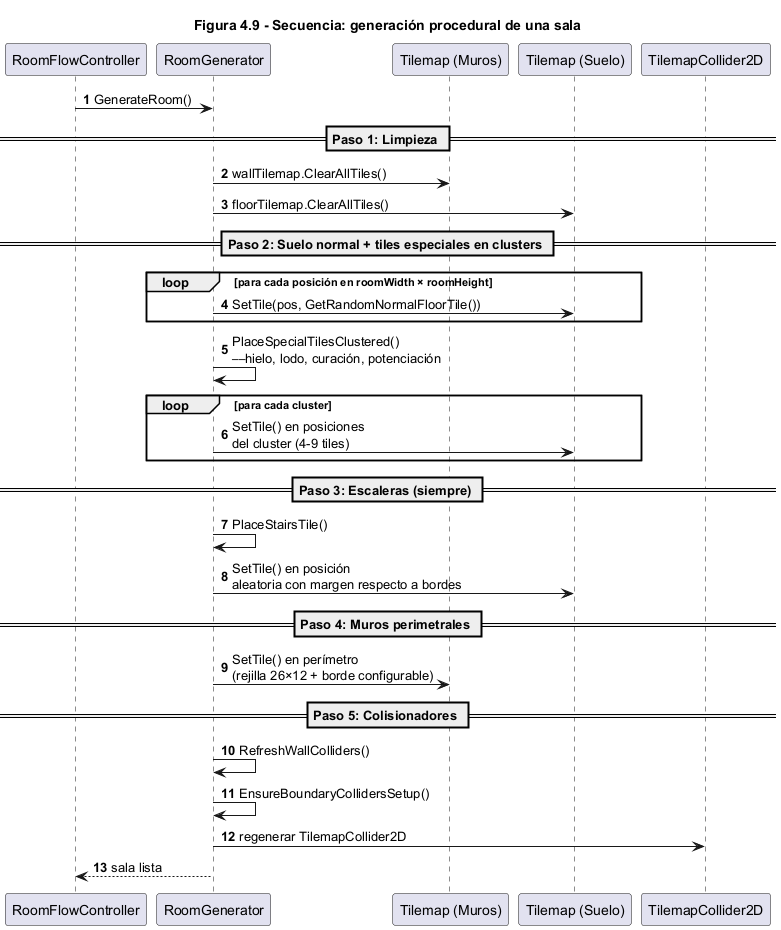
\includegraphics[width=0.95\textwidth,height=0.72\textheight,keepaspectratio]{Figuras/figura4_9_secuencia_generacion_sala.png}
\caption{
Diagrama de secuencia UML de la generación procedural de una sala. \textit{Elaboración propia.}
}
\label{fig:placeholder-19}
\end{center}
\end{figure}

\textbf{Paso 3: Colocación de escaleras.} Las escaleras se colocan en cada sala generada, en una posición aleatoria dentro de una zona segura definida por \texttt{stairsPaddingTiles} (margen configurable respecto a los bordes). El método \texttt{PlaceStairsTile()} aplica el margen sobre el rango de la rejilla y selecciona un punto aleatorio con \texttt{Random.Range}; si el padding es mayor que el espacio disponible, usa el centro como posición de respaldo. Las escaleras permanecen visibles desde el primer momento, pero el jugador no puede interactuar con ellas hasta que la sala se completa.

\textbf{Paso 4: Generación de muros perimetrales.} Se itera sobre las posiciones del perímetro de la rejilla y se coloca un tile de muro en cada posición mediante \texttt{wallTilemap.SetTile()}, creando un recinto cerrado con colisionadores automáticos. El grosor del borde es configurable mediante \texttt{wallBorderThicknessTiles}.

\textbf{Paso 5: Actualización de colisionadores.} Se refresca el \texttt{TilemapCollider2D} de los muros mediante \texttt{RefreshWallColliders()}, y se garantiza la contención del jugador mediante \texttt{EnsureBoundaryCollidersSetup()}, que mantiene \texttt{BoxCollider2D} adicionales en los cuatro bordes como respaldo.

\subsection{VariantTile: tiles con variantes visuales y selección determinista}


La clase \texttt{VariantTile} extiende \texttt{TileBase} de Unity para soportar múltiples sprites por tile, proporcionando variedad visual sin afectar a la jugabilidad. Se seleccionó un sistema de \textit{hash} determinista frente a la alternativa de selección aleatoria pura (\texttt{Random.Range}) porque esta última habría producido cambios visuales cada vez que el \textit{tilemap} se redibuja (por ejemplo, al redimensionar la ventana del editor o al ocultar y mostrar la cámara), generando un efecto de parpadeo visual perceptible por el jugador:

\begin{lstlisting}
public class VariantTile : TileBase {
    public Sprite[] variants;        // Array de variantes visuales para este tipo de tile
    public bool deterministic = true;
    public int seed = 1337;
    public TileEffect tileEffect;    // Efecto asociado (hielo, lodo, curacion, etc.)
    
    public override void GetTileData(Vector3Int position, ITilemap tilemap, 
                                      ref TileData tileData) {
        if (variants != null && variants.Length > 0) {
            int index;
            if (deterministic) {
                unchecked {
                    int hash = seed;
                    hash = hash * 31 + position.x;
                    hash = hash * 17 + position.y;
                    if (position.x != 0) hash ^= position.x << 2;
                    if (position.y != 0) hash ^= position.y << 5;
                    if (hash < 0) hash = -hash;
                    index = hash % variants.Length;
                }
            } else {
                index = Random.Range(0, variants.Length);
            }

            tileData.sprite = variants[index];
        }
    }
}
\end{lstlisting}


Línea por línea:

\begin{itemize}
\item \texttt{public Sprite[] variants}: array configurado desde el inspector de Unity que contiene las variantes visuales de un mismo tipo de tile.
\item \texttt{public bool deterministic}: habilita la selección determinista (estable) de sprite por posición. Si se desactiva, el sprite se selecciona de forma pseudoaleatoria, lo que puede producir variaciones visuales entre repintados.
\item \texttt{public int seed}: semilla adicional que permite variar la distribución sin perder determinismo.
\item \texttt{unchecked { ... }}: asegura que la aritmética de enteros permite desbordamientos sin lanzar excepciones, lo que se utiliza como parte de la mezcla del hash.
\item \texttt{hash = hash \textit{ 31 + position.x; hash = hash } 17 + position.y; ... index = hash \% variants.Length}: cálculo de un hash simple que mezcla la semilla y las coordenadas del tile para obtener un índice estable dentro del rango de variantes.
\end{itemize}

\subsection{TileEffect: efectos de tiles}


Los efectos de tiles se definen como \textit{ScriptableObjects}, lo que permite crear y configurar nuevos efectos desde el inspector de Unity sin modificar el código:

\begin{lstlisting}
[CreateAssetMenu(menuName = "Tiles/TileEffect")]
public class TileEffect : ScriptableObject {
    public string tileName;
    public TileEffectType effectType = TileEffectType.None;
    
    public int healthChange = 0;
    public float speedMultiplier = 1f;
    public float effectDuration = 0f;
    
    public float tickRate = 1f;
    public bool continuous = false;
    
    public Color tintColor = Color.white;
    public GameObject vfxPrefab;
}
\end{lstlisting}


La enumeración \texttt{TileEffectType} define los tipos de efecto posibles:

\begin{lstlisting}
public enum TileEffectType {
    None,       // Sin efecto
    Heal,       // Restaura vida
    Damage,     // Inflige dano
    SpeedUp,    // Incrementa velocidad
    SpeedDown,  // Reduce velocidad
    Ice,        // Tile de hielo
    Mud,        // Tile de lodo
    PowerUp     // Incrementa dano
}
\end{lstlisting}


\subsection{FloorTileManager: aplicación de efectos}


El \texttt{FloorTileManager} detecta sobre qué tile se encuentra el jugador en cada fotograma y aplica el efecto correspondiente:

\begin{lstlisting}
void Update() {
    if (floorTilemap == null || playerTransform == null) return;
    
    Vector3Int tilePos = floorTilemap.WorldToCell(playerTransform.position);
    
    if (tilePos != currentTilePos) {
        OnExitTile();
        currentTilePos = tilePos;
        OnEnterTile();
    }
    
    if (currentEffect?.continuous == true) {
        if (Time.time >= lastEffectTime + currentEffect.tickRate) {
            ApplyEffect(currentEffect);
            lastEffectTime = Time.time;
        }
    }
}
\end{lstlisting}


La conversión de la posición del jugador en coordenadas de mundo a coordenadas de tile se realiza mediante \texttt{WorldToCell}. Cuando el jugador cambia de tile, se ejecutan las funciones de salida del tile anterior y entrada al nuevo tile. Para los efectos con el indicador (\textit{flag}) \texttt{continuous} activado, el efecto se aplica periódicamente según la frecuencia definida en \texttt{tickRate}.

\textbf{Seguimiento visual de efectos.} Al instanciar los efectos visuales (VFX) de un tile, se añade el componente \texttt{VFXFollower} al objeto instanciado para que el efecto visual siga la posición de la entidad afectada (jugador o enemigo). Sin este componente, el VFX quedaría fijo en la posición de instanciación mientras la entidad se desplaza, produciendo una desincronización visual.

\textbf{Persistencia de efectos de velocidad.} Los efectos de modificación de velocidad (hielo, lodo) persisten durante un periodo configurable tras abandonar el tile, evitando que el efecto desaparezca bruscamente:

\begin{lstlisting}
private void ApplySpeedModifier(float multiplier) {
    if (playerController == null) return;
    playerController.SetSpeedMultiplier(multiplier);
    hasSpeedModifier = true;
}

private IEnumerator RemoveSpeedAfterDelay(float seconds) {
    yield return new WaitForSeconds(seconds);
    
    if (hasSpeedModifier && playerController != null) {
        playerController.ResetSpeed();
        hasSpeedModifier = false;
    }
}
\end{lstlisting}


La separación de responsabilidades es deliberada: \texttt{ApplySpeedModifier} solo aplica el multiplicador al controlador del jugador, mientras que la persistencia del efecto tras abandonar el tile se gestiona en el bloque \texttt{ApplyEffect()}, donde se lanza la corutina \texttt{RemoveSpeedAfterDelay(persistEffectSeconds)} si el tiempo de persistencia es mayor que cero.

\textbf{Integración con enemigos.} Los efectos de velocidad de los tiles también se aplican a los enemigos mediante el componente \texttt{EnemyTileEffectReceiver}, que se añade automáticamente a cada enemigo al ser instanciado por el \texttt{EnemyManager}. Este componente consulta el tile sobre el que se encuentra el enemigo y aplica el multiplicador de velocidad correspondiente a través de \texttt{Enemy.SetTileSpeedMultiplier()}, lo que permite al jugador utilizar estas zonas de forma estratégica.

\subsection{DamageBoostManager: bonificación de daño}


El \texttt{DamageBoostManager} gestiona las bonificaciones de daño otorgadas por los tiles de potenciación. Implementa el patrón \textit{Singleton} y soporta bonificaciones permanentes y temporales:

\begin{lstlisting}
public void AddDamageBoostTimed(int amount, float duration) {
    if (duration <= 0f) {
        AddDamageBoost(amount);  // Permanente
        return;
    }
    
    AddDamageBoost(amount);
    StartCoroutine(RemoveDamageBoostAfterDelay(amount, duration));
}

public int GetBoostedDamage(int baseDamage) {
    return baseDamage + globalDamageBoost;
}
\end{lstlisting}


Los proyectiles consultan al \texttt{DamageBoostManager} en su inicialización para calcular su daño efectivo, lo que permite que la bonificación se aplique de forma global y coherente a todas las fuentes de daño del jugador.



\section{Sistema de gestión de salas}


\textbf{Evolución iterativa.} El sistema de gestión de salas se vio directamente afectado por el rediseño de la generación procedural. Cuando cada sala era una escena independiente, el \texttt{RoomController} no existía como tal: la lógica de escaleras y progresión residía en scripts de cada escena. Al consolidar todo el juego en una única escena, se creó el \texttt{RoomController} como componente central para gestionar la detección de entrada del jugador, el bloqueo de escaleras durante el combate y la detección de sala completada.

\subsection{RoomController: control de sala individual}


El \texttt{RoomController} gestiona el ciclo de vida de una sala individual: la detección de entrada del jugador, la activación de la aparición de enemigos, el bloqueo de escaleras durante el combate y la detección de sala completada.

\begin{lstlisting}
void OnTriggerEnter2D(Collider2D other) {
    if (other.CompareTag("Player")) {
        playerInside = true;
        
        if (!isCleared) {
            CloseAllDoors();
        }
    }
}
\end{lstlisting}


Al detectar la entrada del jugador mediante el sistema de \textit{triggers} de Unity, el controlador bloquea las escaleras de la sala y activa la aparición de enemigos. Las escaleras permanecen bloqueadas hasta que todos los enemigos han sido eliminados, momento en el cual se habilitan automáticamente para permitir la progresión.

\begin{figure}[H]
\begin{center}
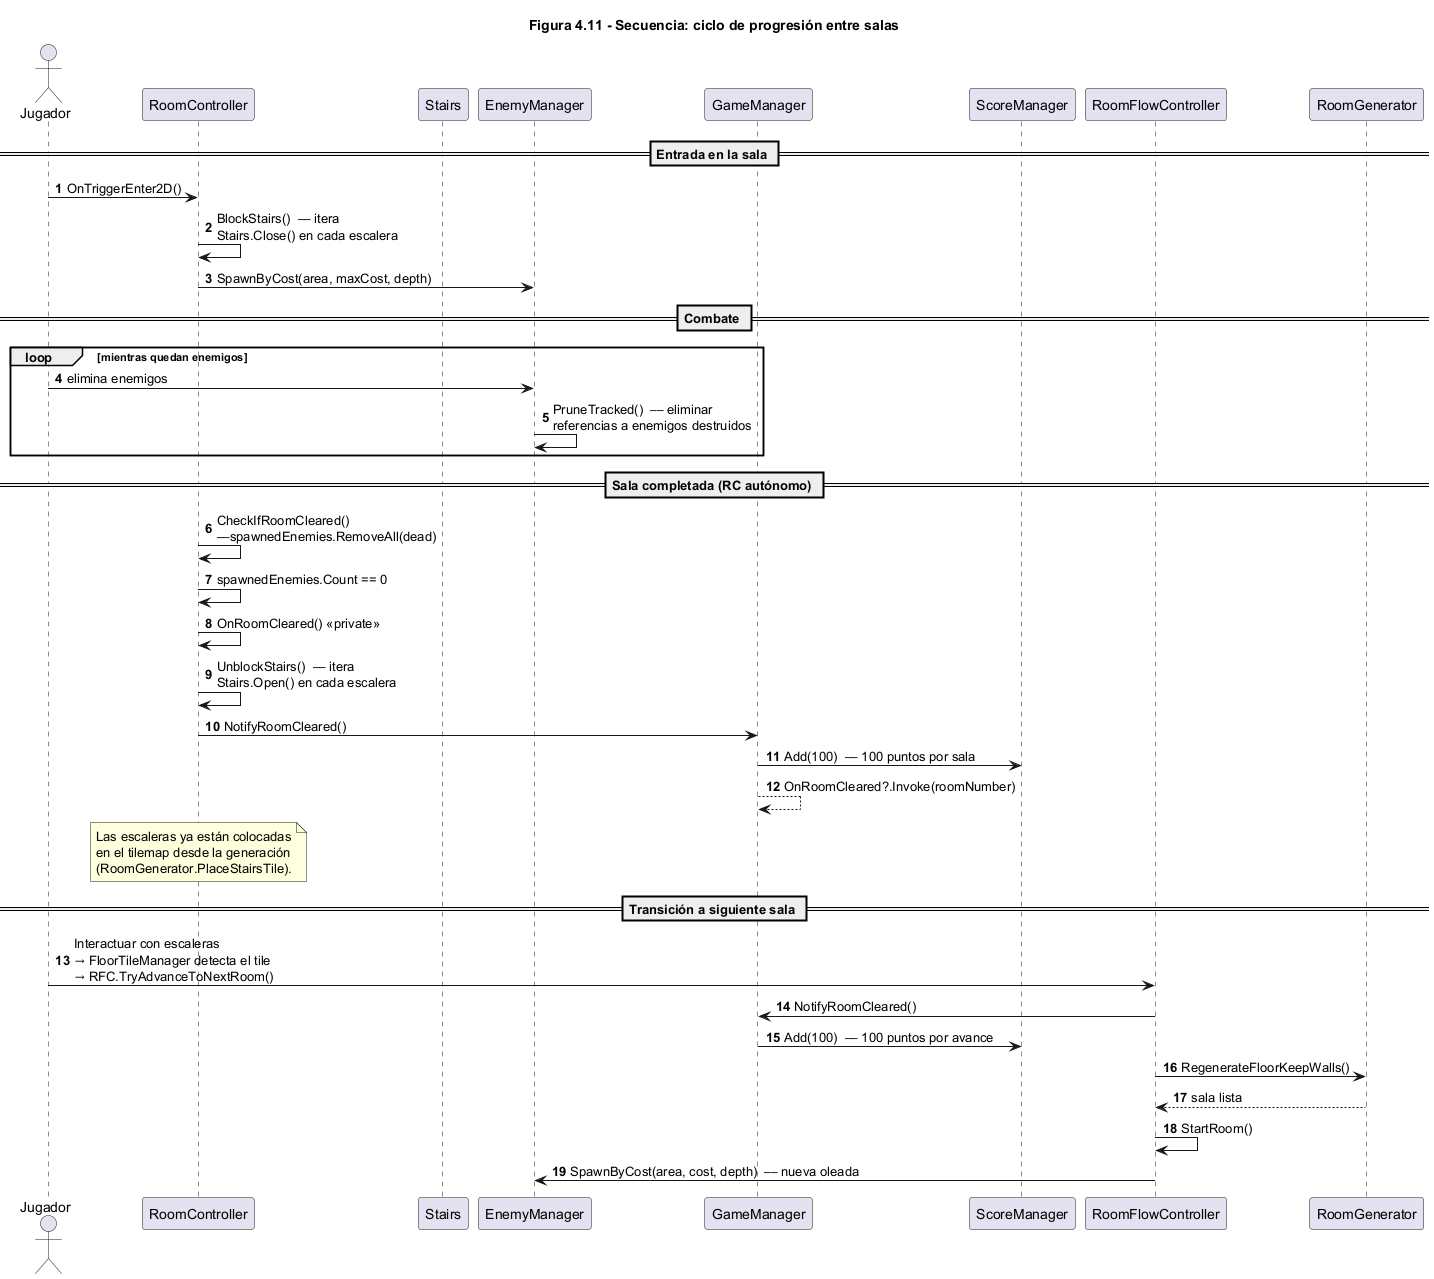
\includegraphics[width=0.95\textwidth,height=0.72\textheight,keepaspectratio]{Figuras/figura4_11_secuencia_progresion_salas.png}
\caption{
Diagrama de secuencia UML del ciclo de progresión entre salas. \textit{Elaboración propia.}
}
\label{fig:placeholder-21}
\end{center}
\end{figure}


\subsection{Stairs: lógica de escaleras}


El componente de escaleras (implementado como clase \texttt{Door} por cuestiones de diseño) gestiona el estado visual y funcional de acceso:

\begin{lstlisting}
public void Open(bool playEffects = true) {
    if (isOpen) return;
    isOpen = true;
    doorCollider.enabled = false;
}

public void Close(bool playEffects = true) {
    isOpen = false;
    doorCollider.enabled = true;
}
\end{lstlisting}


La escalera alterna entre un estado bloqueado y un estado habilitado.



\section{Sistema de interfaz de usuario}


\textbf{Evolución iterativa.} La interfaz de usuario fue el último subsistema en integrarse con el patrón \textit{Observer}. En las primeras iteraciones, cada componente de UI consultaba directamente al \texttt{GameManager} en su método \texttt{Update()} (lectura síncrona por sondeo), lo que generaba comprobaciones redundantes en cada fotograma y acoplaba la interfaz con la implementación interna del gestor. La adopción del patrón \textit{Observer} -- suscripción al evento \texttt{OnGameStateChanged} -- eliminó esta dependencia: los paneles de pausa, derrota y victoria solo ejecutan lógica cuando reciben una notificación de cambio de estado, no en cada fotograma. El sistema de corazones evolucionó de una implementación estática (número fijo de corazones en la escena) a una generación dinámica basada en \texttt{maxHealth}, lo que permitió que las clases de personaje con distinta cantidad de vida máxima se representasen correctamente sin configuración manual.

\subsection{HeartDisplay: representación de vida}


El \texttt{HeartDisplay} proporciona una representación visual dinámica de la vida del jugador mediante iconos de corazones. El sistema crea los corazones de forma dinámica en función de la vida máxima del personaje:

\begin{lstlisting}
public void InitializeHearts(int maxHealth) {
    ClearHearts();
    maxHearts = Mathf.Max(0, maxHealth);
    
    for (int i = 0; i < maxHearts; i++) {
        CreateHeart(i);
    }
}
\end{lstlisting}


La actualización responde a los cambios en la vida del jugador, alternando los sprites de corazón lleno y vacío:

\begin{lstlisting}
public void UpdateHearts(int currentHealth) {
    int clampedHealth = Mathf.Clamp(currentHealth, 0, maxHearts);
    
    for (int i = 0; i < heartImages.Count; i++) {
        Image heartImage = heartImages[i];
        if (heartImage == null) continue;
        
        heartImage.sprite = i < clampedHealth ? heartFull : heartEmpty;
        heartImage.enabled = true;
    }
}
\end{lstlisting}


\subsection{PauseMenu: menú de pausa}


El \texttt{PauseMenu} se suscribe al evento \texttt{OnGameStateChanged} del \texttt{GameManager} y activa o desactiva su panel según el estado actual del juego:

\begin{lstlisting}
void Start() {
    EnsureRuntimeUIIfMissing();
    WireButtonsOnce();
    
    if (pauseMenuPanel != null)
        pauseMenuPanel.SetActive(false);
    
    GameManager.OnGameStateChanged += OnGameStateChanged;
}

private void OnGameStateChanged(GameState newState) {
    EnsureRuntimeUIIfMissing();
    if (pauseMenuPanel == null) return;
    
    bool shouldShow = (newState == GameState.Paused);
    pauseMenuPanel.SetActive(shouldShow);
}
\end{lstlisting}


Este diseño ejemplifica la aplicación del patrón \textit{Observer}: el menú de pausa no consulta activamente el estado del juego, sino que reacciona a la notificación de cambio de estado emitida por el \texttt{GameManager}. Las llamadas a \texttt{EnsureRuntimeUIIfMissing()} y \texttt{WireButtonsOnce()} garantizan que la interfaz de pausa exista y tenga sus botones configurados incluso cuando el \texttt{PauseMenu} se crea en tiempo de ejecución sin referencias previas asignadas en el inspector. Esto permite añadir o eliminar elementos de interfaz reactivos sin modificar el código del gestor central.

\subsection{Pantallas de fin de partida}


Las pantallas de derrota (\texttt{GameOverScreen}) y victoria (\texttt{VictoryScreen}) se activan automáticamente al cambiar el estado del juego a \texttt{GameOver} o \texttt{Victory}, respectivamente:

\begin{lstlisting}
public void Show() {
    if (victoryPanel == null) return;
    victoryPanel.SetActive(true);
    
    if (scoreText != null && ScoreManager.Instance != null)
        scoreText.text = $"Puntuacion Final: {ScoreManager.Instance.CurrentScore}";
    if (roomsClearedText != null && GameManager.Instance != null)
        roomsClearedText.text = $"Salas limpiadas: {GameManager.Instance.RoomsCleared}";
    if (enemiesKilledText != null && GameManager.Instance != null)
        enemiesKilledText.text = $"Enemigos eliminados: {GameManager.Instance.EnemiesKilled}";
    if (timeText != null) {
        float runTime = Time.time - runStartTime;
        int minutes = Mathf.FloorToInt(runTime / 60f);
        int seconds = Mathf.FloorToInt(runTime % 60f);
        timeText.text = $"Tiempo: {minutes:00}:{seconds:00}";
    }
}
\end{lstlisting}


Ambas pantallas muestran un texto que representa el final de la partida y redirigen al menú principal tras un tiempo.


\begin{figure}[H]
\begin{center}
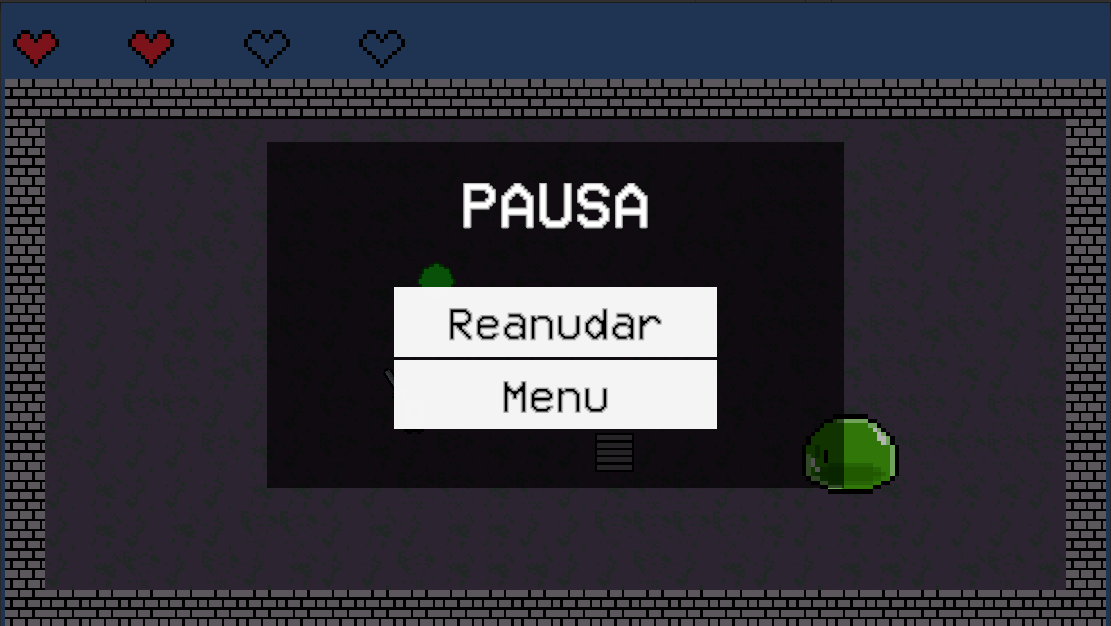
\includegraphics[width=0.9\textwidth]{Figuras/captura_14.png}
\caption{Captura de pantalla del menú de pausa de \textit{Ascension}, mostrando las opciones de reanudar y menú principal. \textit{Elaboración propia.}}
\label{fig:placeholder-23}
\end{center}
\end{figure}

\subsection{ScoreboardMenuUI: historial de puntuaciones}


El historial de puntuaciones se genera dinámicamente a partir de los datos almacenados por el \texttt{ScoreManager}. En lugar de instanciar un \textit{prefab} por cada entrada, el componente utiliza un único campo \texttt{TextMeshProUGUI} -- un sistema de renderizado de texto de alta calidad integrado en Unity que soporta formato enriquecido, sombreado y alineación precisa a nivel de píxel -- y construye todo el listado mediante un \texttt{StringBuilder}, lo que resulta más eficiente en memoria y evita la necesidad de gestionar la destrucción de objetos instanciados:

\begin{lstlisting}
public void Refresh() {
    if (listText == null) return;
    
    var sb = new StringBuilder();
    var entries = ScoreManager.Instance != null
                     ? ScoreManager.Instance.GetHistory() : null;
    
    sb.AppendLine("SCORES");
    sb.AppendLine("------");
    
    if (entries == null || entries.Count == 0) {
        sb.AppendLine("(sin partidas guardadas)");
        listText.text = sb.ToString();
        return;
    }
    
    int rank = 1;
    foreach (var e in entries) {
        sb.Append(rank).Append(". ")
          .Append(e.score).Append(" pts")
          .Append(" | ").Append(e.result)
          .Append(" | ").Append(e.playerClass)
          .Append(" | R ").Append(e.roomsCleared)
          .Append(" | K ").Append(e.enemiesKilled)
          .AppendLine();
        rank++;
    }
    
    listText.text = sb.ToString();
}
\end{lstlisting}




\section{Sistemas preparados para extensión}


\textbf{Evolución iterativa.} Ambos sistemas descritos en esta sección (jefes con fases y generación procedural de armas) se desarrollaron como prototipos funcionales durante iteraciones intermedias del proyecto. La decisión de no integrarlos en el bucle de juego final se tomó tras evaluar la prioridad de las tareas restantes: el equilibrado de dificultad de los jefes con fases múltiples y la interfaz de recogida de armas generadas requerían un volumen de trabajo que habría comprometido la entrega de los subsistemas prioritarios. Se optó por mantener el código desarrollado como extensión documentada, alineándose con el principio de apertura-cierre: la arquitectura permite su integración futura sin modificar los subsistemas existentes.

La arquitectura del proyecto se ha diseñado teniendo en cuenta la extensibilidad. Se han desarrollado dos sistemas cuya estructura se ha preparado a nivel de código pero que no se encuentran completamente integrados en el bucle de juego al cierre del presente trabajo:

\subsection{Sistema de jefes con fases múltiples}


Se ha desarrollado el componente \texttt{BossController} que implementa un sistema de jefes con dos fases diferenciadas basadas en el porcentaje de vida restante. El diseño contempla la transición automática a la segunda fase al alcanzar el 50 \% de vida, con cambios en la cadencia de ataque, la velocidad de movimiento y los patrones de disparo. No obstante, al no encontrarse integrado en el bucle de progresión de salas, su funcionamiento en una partida completa no se ha verificado de forma consistente; su integración requiere trabajo adicional en el equilibrado de dificultad y en la definición de patrones de ataque más variados.

\subsection{Generación procedural de armas con rareza}


Se ha desarrollado el componente \texttt{WeaponGenerator} que implementa un sistema de generación procedural de armas con cuatro niveles de rareza (Común, Poco Común, Raro, Legendario) y escalado de estadísticas basado en la profundidad de la mazmorra. Al no encontrarse integrado en el flujo de juego -- aparición de armas como objetos recogibles en las salas --, su funcionamiento en una partida completa no se ha verificado de forma consistente; la integración constituye un desarrollo pendiente para futuras iteraciones del proyecto.

Estos dos sistemas se analizan con mayor detalle en el apartado de líneas de trabajo futuro.



\section{Compilación y ejecución}


\textbf{Evolución iterativa.} Las primeras versiones del proyecto se ejecutaban exclusivamente desde el editor de Unity durante el desarrollo. La generación del ejecutable final se realizó una vez estabilizados los subsistemas principales, verificando que el comportamiento del juego compilado fuese idéntico al observado en el editor.

\subsection{Proceso de compilación}


La compilación del proyecto se realiza desde la ventana \textit{Build Profiles} del editor de Unity (\texttt{File > Build Profiles}). La configuración utilizada es la siguiente:

\begin{itemize}
\item \textbf{Motor:} Unity 6 (versión 6000.2.7f2).
\item \textbf{Plataforma objetivo:} Windows, arquitectura Intel 64-bit.
\item \textbf{Backend de scripting:} Mono (compatible con .NET Standard 2.1).
\item \textbf{Escenas incluidas en el \textit{build}:} se incluyen las tres escenas del proyecto en el orden definido por el flujo de juego:
\end{itemize}

\begin{enumerate}
\item \texttt{Scenes/MainMenu} (índice 0) -- menú principal.
\item \texttt{Scenes/ClassSelection} (índice 1) -- pantalla de selección de clase.
\item \texttt{Scenes/GameScene} (índice 2) -- escena principal de juego.
\end{enumerate}

\begin{itemize}
\item \textbf{Opciones de compilación desactivadas:} \textit{Copy PDB files}, \textit{Create Visual Studio Solution} y \textit{Development Build}. Esto genera un ejecutable de producción optimizado, sin símbolos de depuración ni herramientas de \textit{profiling}.
\end{itemize}

El orden de las escenas es relevante: Unity carga automáticamente la escena con índice 0 al iniciar el ejecutable, por lo que \texttt{MainMenu} debe ocupar la primera posición para que el jugador acceda al menú principal al arrancar el juego.

Para generar el ejecutable, se selecciona la plataforma \textit{Windows} en la ventana \textit{Build Profiles}, se verifica que las tres escenas estén incluidas y ordenadas correctamente, y se pulsa \textit{Build}. Unity compila los scripts de C\# mediante el compilador Roslyn integrado, empaqueta los activos del proyecto (sprites, tilemaps, prefabs, ScriptableObjects) en archivos binarios optimizados y genera el ejecutable junto con sus dependencias.

\subsection{Estructura del ejecutable}


El proceso de compilación genera la siguiente estructura de archivos en el directorio de salida:

\begin{lstlisting}
Build/
 Ascension.exe                           Ejecutable principal
 UnityPlayer.dll                         Motor de ejecucion de Unity
 UnityCrashHandler64.exe                 Gestor de errores criticos
 Ascension_Data/                         Activos compilados del proyecto
    level0, level1, level2              Escenas empaquetadas
    resources.assets                    Activos marcados como Resources
    sharedassets02.assets              Activos especificos de cada escena
    globalgamemanagers                  Configuracion global del proyecto
    Managed/                            Ensamblados .NET compilados
    Plugins/x86_64/                     Bibliotecas nativas
 MonoBleedingEdge/                       Runtime de Mono (.NET)
 D3D12/                                  Bibliotecas de renderizado DirectX 12
\end{lstlisting}


Los archivos \texttt{level0}, \texttt{level1} y \texttt{level2} corresponden a las tres escenas del proyecto en el orden definido en \textit{Build Profiles}. El directorio \texttt{Managed/} contiene los ensamblados compilados a partir de los scripts de C\# del proyecto (\texttt{Assembly-CSharp.dll}) y las bibliotecas del framework de Unity.

\subsection{Ejecución del juego}


Para ejecutar el juego, el usuario debe:

\begin{enumerate}
\item Copiar la carpeta \texttt{Build/} completa a la ubicación deseada, manteniendo la estructura de directorios intacta.
\item Ejecutar \texttt{Ascension.exe}.
\end{enumerate}

No es necesario instalar Unity ni ningún componente adicional: el ejecutable incluye el \textit{runtime} de Mono y las bibliotecas del motor de Unity necesarias para la ejecución autónoma. El juego se inicia mostrando la pantalla del menú principal, desde la cual el jugador puede acceder a la selección de clase, consultar el historial de puntuaciones o salir del juego.

\textbf{Requisitos mínimos del sistema:}

\begin{itemize}
\item Sistema operativo: Windows 10 (64 bits) o posterior.
\item Procesador: compatible con x86_64.
\item Memoria: 4 GB de RAM.
\item Gráficos: compatible con DirectX 11 o DirectX 12.
\item Almacenamiento: aproximadamente 100 MB de espacio en disco.
\end{itemize}

\chapter{Conclusiones y trabajo futuro}


El presente capítulo recoge las conclusiones del trabajo realizado, evaluando el grado de cumplimiento de los objetivos establecidos, identificando las limitaciones del proyecto y proponiendo líneas de trabajo futuro.



\section{Cumplimiento de objetivos}


A continuación se evalúa el grado de cumplimiento de cada uno de los objetivos específicos definidos en la introducción.

\textbf{OE-1. Diseñar e implementar una arquitectura modular basada en patrones de diseño.} Se considera cumplido. La arquitectura del proyecto aplica patrones de diseño de forma consistente, en particular \textit{Singleton}, \textit{Observer}, \textit{Strategy} y \textit{Template Method}. Adicionalmente, se emplean mecanismos propios de Unity (sistema de componentes) y una máquina de estados para la coordinación del flujo del juego. La modularidad y la separación entre lógica y presentación se verificaron inicialmente de forma manual durante el desarrollo y, posteriormente, mediante el análisis estático automatizado, que confirmó la presencia de los cuatro \textit{Singletons} documentados, las cuatro declaraciones de eventos \textit{Observer} y las cinco clases \texttt{ScriptableObject} previstas.

\textbf{OE-2. Diseñar e implementar un sistema de generación procedural de salas.} Se considera cumplido. Se ha desarrollado el componente \texttt{RoomGenerator}, que genera salas de $26 \times 12$ tiles con muros perimetrales, tiles normales con variantes visuales y tiles especiales distribuidos mediante un algoritmo de expansión por \textit{clusters}. La generación introduce variabilidad en la disposición de elementos entre partidas.

\textbf{OE-3. Desarrollar una inteligencia artificial diferenciada para al menos tres tipos de enemigo.} Se considera cumplido. Se han implementado tres tipos de enemigo con comportamientos distintos: el slime verde (ataque a distancia con mantenimiento de distancia objetivo), el slime rojo (persecución directa) y el slime azul (aproximación por saltos, desplazamientos rápidos o \textit{dash}). Los tres tipos aplican un periodo de gracia tras su aparición y reaccionan a tiles que modifican la velocidad. Asimismo, se ha implementado un sistema de enemigos especiales con atributos escalados que actúan como jefes periódicos. Su diseño e implementación incluyen la formalización de estados y transiciones (FSM) y fragmentos de código del bucle de IA. La comprobación funcional se realizó en \textit{Play Mode} (editor de Unity) observando transiciones de estado, ventanas de gracia y reacción a tiles; adicionalmente, el \textit{stress test} aporta evidencia de estabilidad del subsistema bajo alta carga de instanciación y destrucción de enemigos.

\textbf{OE-4. Crear un sistema de armas con mecánicas de combate cuerpo a cuerpo y a distancia.} Se considera cumplido. El sistema de armas, basado en el patrón \textit{Strategy}, ofrece dos modalidades de combate diferenciadas: \texttt{MeleeWeapon} (ataque de barrido con animación procedural sinusoidal) y \texttt{RangedWeapon} (disparo de proyectiles dirigidos hacia el cursor). La implementación abarca la clase base \texttt{Weapon}, las subclases, los proyectiles, los datos \texttt{WeaponData} y el flujo de daño hasta la puntuación. La verificación se realizó de forma manual en el editor de Unity, comprobando: activación del ataque, generación de proyectiles, colisiones/hitboxes, \textit{cooldowns} y aplicación de daño. De forma complementaria, los escenarios de estrés ejercitan el uso intensivo de instanciación/destrucción asociada a proyectiles y enemigos.

\textbf{OE-5. Implementar un sistema de tiles con efectos que modifiquen la jugabilidad.} Se considera cumplido. Se han desarrollado cuatro tipos de tiles con efectos: hielo (incrementa velocidad), lodo (reduce velocidad), curación (restaura vida) y potenciación (incrementa daño). Los efectos se configuran mediante \textit{ScriptableObjects} y afectan tanto al jugador como a los enemigos. La distribución se realiza mediante el algoritmo de expansión por \textit{clusters} con probabilidades configurables. Su comprobación se realizó verificando manualmente en el editor de Unity (aplicación/retirada de efectos durante la partida).

\textbf{OE-6. Implementar un sistema de persistencia de puntuaciones y estadísticas.} Se considera cumplido. El \texttt{ScoreManager} gestiona la puntuación en tiempo real, el registro de estadísticas por partida y la persistencia del historial mediante \texttt{PlayerPrefs} (almacenamiento local clave–valor) y serialización JSON (formato de texto estructurado). El diseño y la implementación abarcan la persistencia y estructura del historial, y se muestra el consumo de estos datos en la interfaz del menú principal. El historial almacena hasta 30 entradas con puntuación, clase, salas completadas, enemigos eliminados, resultado y marca de tiempo. Su comprobación se realizó de forma manual, ejecutando partidas consecutivas y verificando la persistencia de los datos entre ejecuciones del juego.

\textbf{OE-7. Documentar el proceso de desarrollo y las decisiones técnicas adoptadas.} Se considera cumplido. La memoria describe los requisitos, la arquitectura, los módulos implementados, los patrones de diseño aplicados, los resultados obtenidos, las limitaciones y las líneas de trabajo futuro, apoyándose en diagramas y fragmentos de código. La trazabilidad se apoya en la relación entre los objetivos, las historias de usuario y los criterios de aceptación definidos y la valoración del cumplimiento recogida en este capítulo.

\section{Valoración del trabajo realizado}


El proyecto \textit{Ascension} ha permitido aplicar de forma integrada los conocimientos adquiridos durante el Grado en Ingeniería Informática en áreas como la ingeniería del software, la programación orientada a objetos, la algoritmia y el diseño de sistemas interactivos.

Desde el punto de vista cuantitativo, a fecha de redacción de esta memoria, el directorio \texttt{Assets/Scripts/} contiene \textbf{85} scripts C\# de proyecto con un total de \textbf{12.565} líneas de código. La aportación técnica del trabajo se fundamenta en la implementación e integración de sistemas como la generación procedural de contenido, la inteligencia artificial de los enemigos con tres comportamientos diferenciados y la arquitectura guiada por patrones de diseño.

La utilización de \textit{ScriptableObjects} como mecanismo de separación entre datos y lógica ha permitido iterar sobre el equilibrado del juego -- estadísticas de clases, datos de enemigos, efectos de tiles -- sin recompilar el código fuente en cada modificación.

El proceso de desarrollo ha requerido ciclos de prueba funcional y depuración, con especial atención a la coherencia entre subsistemas (generación procedural, combate, IA, interfaz y persistencia) y a la estabilidad del flujo de juego.



\section{Limitaciones del proyecto}


A pesar de los resultados obtenidos, se han identificado las siguientes limitaciones:

\begin{enumerate}
\item \textbf{Ausencia de sistema de audio.} El proyecto no incluye un sistema de gestión de efectos de sonido ni música. La implementación de un \texttt{AudioManager} centralizado con mezcla de canales constituye una mejora necesaria para proporcionar una experiencia completa.
\item \textbf{Variedad limitada de contenido.} El juego dispone de tres tipos de enemigo y un conjunto reducido de armas. La generación procedural de armas con sistema de rareza (\texttt{WeaponGenerator}) está implementada a nivel de código pero no integrada en el flujo de juego; en consecuencia, su funcionamiento dentro de una partida completa no se ha verificado de forma consistente.
\item \textbf{Sistema de jefes no integrado.} El \texttt{BossController} implementa un sistema de dos fases con patrones de ataque diferenciados, pero no se encuentra integrado en el flujo de juego de la versión actual. En consecuencia, su funcionamiento dentro de una partida completa no ha podido verificarse de forma consistente.
\item \textbf{Ausencia de reutilización de objetos (\textit{object pooling}).} Los proyectiles y efectos visuales se crean y destruyen mediante \texttt{Instantiate} y \texttt{Destroy}, lo que puede generar presión sobre el recolector de basura en situaciones con alto volumen de proyectiles. La implementación de un sistema de reutilización de objetos (\textit{object pooling}) mejoraría el rendimiento en estos escenarios.
\item \textbf{Cobertura de pruebas.} El proyecto no dispone de una suite formal de pruebas unitarias ni de integración con cobertura sistemática de todos los módulos. La implementación de un marco de pruebas más completo mejoraría la detección temprana de regresiones.
\end{enumerate}

\section{Líneas de trabajo futuro}


A partir de las limitaciones identificadas y de las oportunidades de extensión detectadas durante el desarrollo, se proponen las siguientes líneas de trabajo futuro:

\subsection{Integración del sistema de jefes con fases múltiples}


El componente \texttt{BossController} implementa un sistema de dos fases con transición automática al 50 \% de vida. La primera fase presenta ataques moderados con cadencia lenta, mientras que la segunda fase introduce ráfagas de proyectiles a mayor velocidad. La integración completa de este sistema implica:
\begin{itemize}
\item Diseño de patrones de ataque variados para cada fase
\item Equilibrado de las estadísticas del jefe en relación con la profundidad de la partida
\item Implementación de retroalimentación visual y auditiva para la transición de fase
\item Integración con el sistema de puntuación con bonificaciones específicas por derrotar jefes
\end{itemize}

\subsection{Integración del sistema de generación procedural de armas}


El componente \texttt{WeaponGenerator} implementa a nivel de código un sistema de cuatro niveles de rareza (Común con multiplicador $\times 1{,}0$; Poco Común con $\times 1{,}3$; Raro con $\times 1{,}6$; Legendario con $\times 2{,}0$) y escalado de estadísticas basado en la profundidad (+10 \% por nivel). Dado que el sistema no se encuentra integrado en el flujo de juego, su validación se considera pendiente. La integración completa implica:
\begin{itemize}
\item Aparición de armas como objetos recogibles en las salas
\item Sistema de interfaz para comparar armas y decidir si equipar la nueva
\item Retroalimentación visual diferenciada según la rareza del arma
\item Equilibrado de las probabilidades de aparición por profundidad
\end{itemize}

\subsection{Ampliación del contenido}


\begin{itemize}
\item Nuevos tipos de enemigo con comportamientos diferenciados
\item Nuevos tipos de tiles con efectos adicionales (veneno, teletransporte)
\item Nuevos tipos de sala (salas de tesoro, salas de tienda, salas trampa)
\item Sistemas de progresión permanente entre partidas (\textit{meta-progression})
\end{itemize}

\subsection{Mejoras técnicas}


\begin{itemize}
\item Implementación de \textit{object pooling} para proyectiles y efectos visuales
\item Sistema de gestión de audio centralizado
\item Creación de pruebas unitarias y de integración con cobertura sistemática
\item Optimización de rendimiento mediante perfilado con \textit{Unity Profiler}
\item Sistema de guardado y carga del progreso de partida
\end{itemize}

\section{Reflexión final}


El desarrollo del videojuego \textit{Ascension} ha constituido un ejercicio integrador que ha permitido abordar, en un marco práctico, retos técnicos propios del desarrollo de software con múltiples subsistemas: diseño arquitectónico, implementación de algoritmos, aplicación de patrones de diseño y gestión de la calidad del código.

El subgénero \textit{roguelike} constituye un contexto adecuado para la demostración de competencias de ingeniería del software, ya que exige la integración de múltiples subsistemas -- generación procedural, inteligencia artificial, gestión de estados e interacción con el entorno -- en un sistema cohesionado y funcional.

La arquitectura modular adoptada, fundamentada en patrones de diseño de la ingeniería del software y en mecanismos propios de Unity (\textit{ScriptableObjects} y sistema de componentes), permite extender el sistema mediante la incorporación de nuevos subsistemas. En particular, se han implementado estructuras para un sistema de jefes con fases y para la generación procedural de armas, cuya integración en el flujo de juego se identifica como trabajo futuro.









% ========= BIBLIOGRAFÍA =========
\addcontentsline{toc}{section}{Bibliografía}
\bibliography{referencias}

% ========= ANEXOS =========
\appendix
\appendix
\chapter{Artefactos software}

Este apéndice recoge los principales artefactos software generados durante el desarrollo del Trabajo de Fin de Grado. Su inclusión complementa la memoria principal con una vista técnica de los entregables reales del proyecto.

Además, se proporciona un enlace al repositorio de GitHub donde se encuentra el código fuente completo del videojuego: https://github.com/nsh255/ascension.git

\section{Estructura del proyecto}

El proyecto se ha desarrollado en Unity con una organización modular orientada a responsabilidades. A nivel práctico, los artefactos más relevantes del repositorio son:

\begin{itemize}
    \item \textbf{Ascension/Ascension/Assets/Scripts}: lógica principal del juego en C\#, organizada por subsistemas (Core, Player, Enemies, Weapons, UI, Tiles y LevelGeneration).
    \item \textbf{Ascension/Ascension/Assets/Prefabs}: objetos reutilizables del juego (jugador, enemigos, armas, escaleras y elementos de sala).
    \item \textbf{Ascension/Ascension/Assets/Scenes}: escenas del flujo completo (menú principal, selección de class y escena principal de juego).
    \item \textbf{Ascension/Ascension/LATEX/Diagramas}: fuentes PlantUML de los diagramas técnicos utilizados en la memoria.
    \item \textbf{Ascension/Ascension/LATEX}: memoria final, bibliografía y figuras integradas para compilación del documento.
\end{itemize}

Esta estructura ha permitido mantener bajo acoplamiento entre módulos y facilitar la iteración de mecánicas.

\section{Arquitectura del sistema}

La arquitectura del videojuego se basa en un enfoque modular con patrones \textit{Singleton}, \textit{Observer}, \textit{Strategy} y \textit{Template Method}. Entre los subsistemas implementados destacan:

\begin{itemize}
    \item Gestión de estado global de partida (\texttt{GameManager}).
    \item Progresión de salas y coordinación de oleadas (\texttt{RoomFlowController} y \texttt{EnemyManager}).
    \item Generación procedural de salas y tiles con efectos (\texttt{RoomGenerator} y \texttt{FloorTileManager}).
    \item Sistema de jugador, combate y armas (cuerpo a cuerpo y a distancia).
    \item Interfaz de usuario y persistencia de puntuaciones.
\end{itemize}

Con el objetivo de aportar una visión estructural del sistema, en el siguiente apartado se incluyen los diagramas UML utilizados durante el diseño.

\section{Diagramas del sistema}

La Figura \ref{fig:clases} muestra el diagrama de clases del sistema, en el que se representan las principales entidades del videojuego y sus relaciones. Este diagrama permite comprender la organización interna del código y la separación de responsabilidades entre los distintos componentes.

\clearpage
\begin{sidewaysfigure}
    \begin{center}
    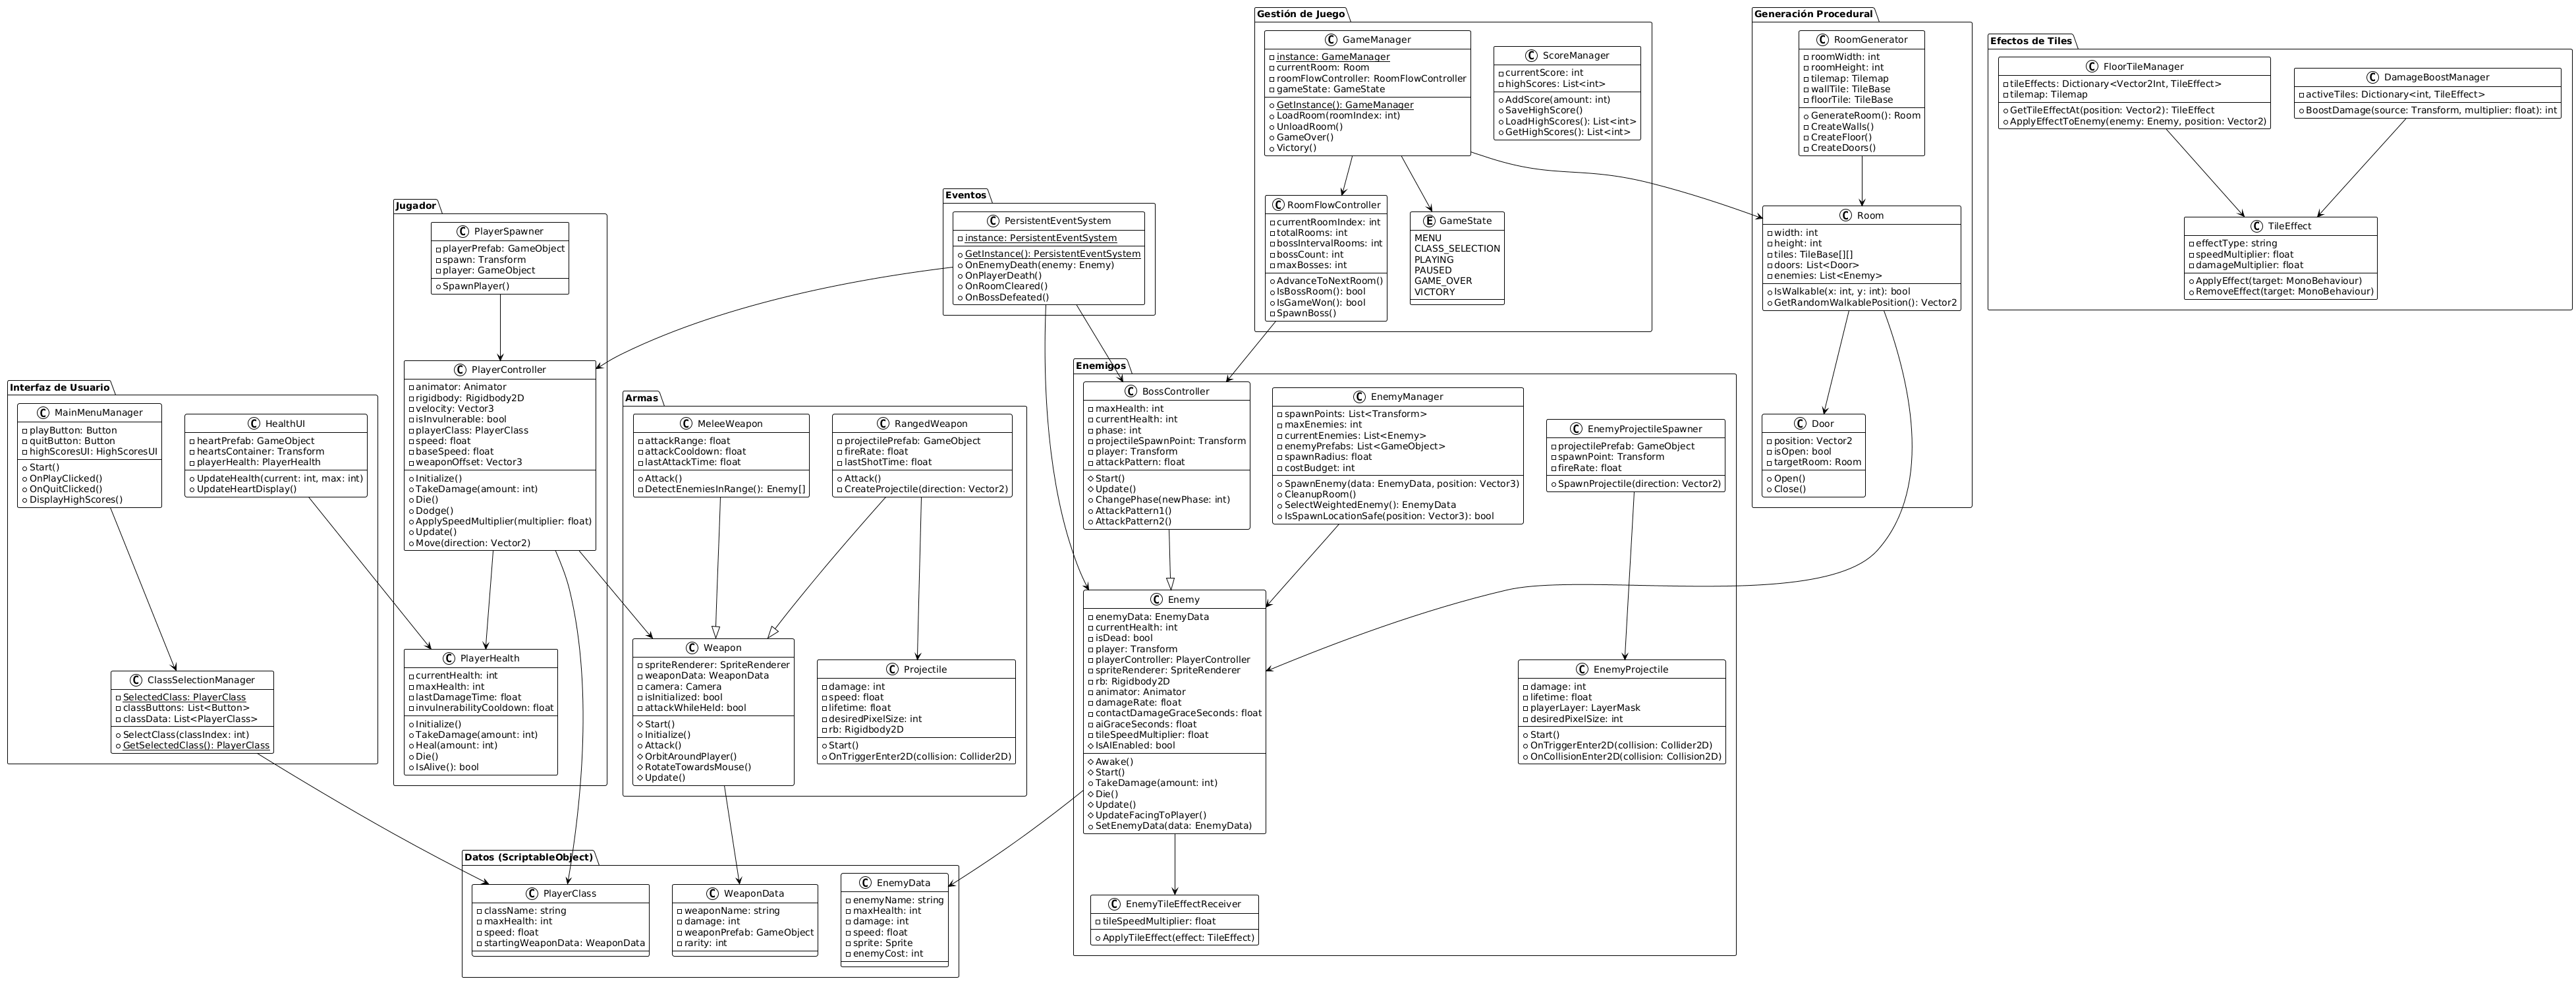
\includegraphics[width=\textheight]{Figuras/Diagrama_Clases.png}
    \caption{Diagrama de clases del sistema}
    \label{fig:clases}
    \end{center}
\end{sidewaysfigure}
\clearpage

Por otro lado, la Figura \ref{fig:casosuso} presenta el diagrama de casos de uso, que describe las interacciones principales entre el jugador y el sistema, proporcionando una visión funcional del comportamiento esperado del videojuego.

\clearpage
\begin{sidewaysfigure}
    \begin{center}
    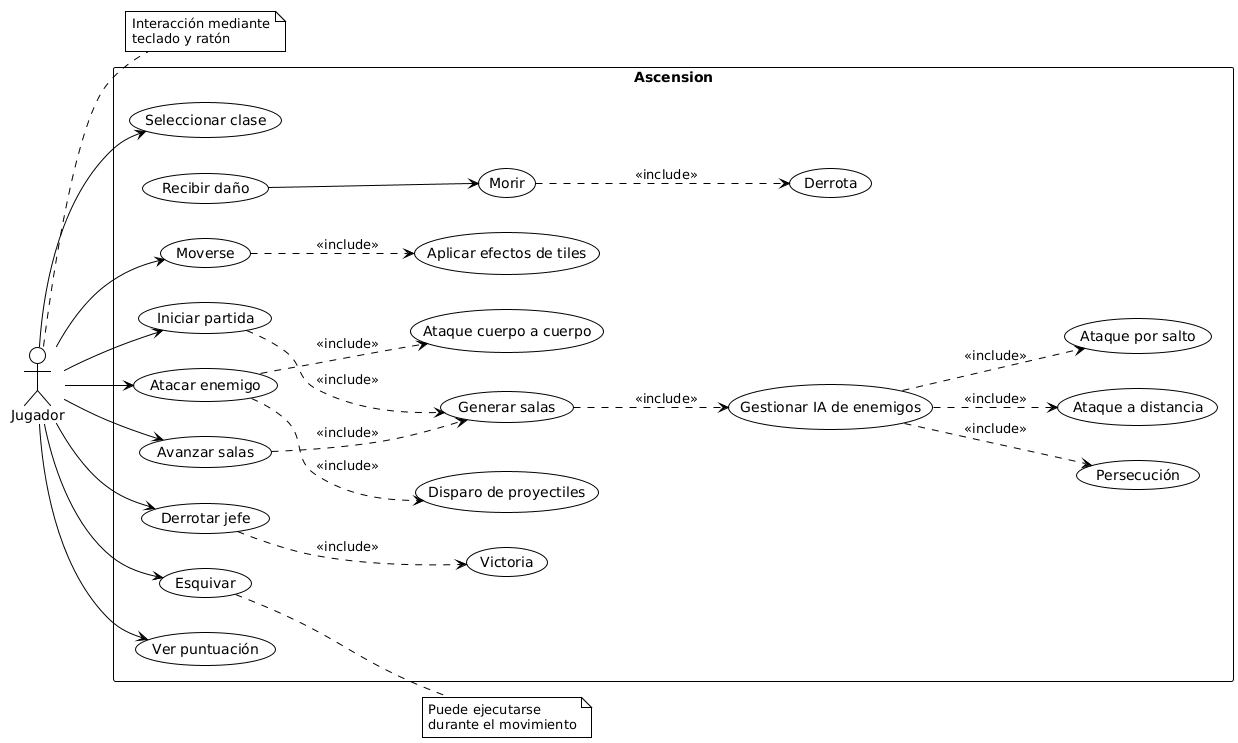
\includegraphics[width=\textheight]{Figuras/Diagrama_Casos_Uso.png}
    \caption{Diagrama de casos de uso del sistema}
    \label{fig:casosuso}
    \end{center}
\end{sidewaysfigure}
\clearpage



% ========= CONTRAPORTADA =========
\backmatter
\input{contra}

\end{document}
